\documentclass[8.5pt,twoside,twocolumn]{article}
%% CHECK: Remove all ``CHECK'' comments by solving their problems
%% CHECK: Maybe better to include that sometimes by graphs sets are meant,
 %        sometimes sums. 
%% CHECK: Graph alignment with array environment.
%% CHECK: Mengen und Teilmengen schwierig. Müsste ja eigentlich immer sowas sein wie
 %        M \in P(\Ga).
\usepackage[utf8]{inputenc}
\usepackage{MyChem}
\usepackage{MyStandard}
\usepackage{courier}
\usepackage{booktabs}
\usepackage{tabto}
\usepackage{tabu}
\usepackage{longtable}
\usepackage{enumerate}
\usepackage{tikz}
\usetikzlibrary{patterns,calc,decorations.pathmorphing}

\makeatletter
\newcommand{\subalign}[1]{%
  \vcenter{%
    \Let@ \restore@math@cr \default@tag
    \baselineskip\fontdimen10 \scriptfont\tw@
    \advance\baselineskip\fontdimen12 \scriptfont\tw@
    \lineskip\thr@@\fontdimen8 \scriptfont\thr@@
    \lineskiplimit\lineskip
    \ialign{\hfil$\m@th\scriptstyle##$&$\m@th\scriptstyle{}##$\crcr
      #1\crcr
    }%
  }
}
\makeatother

\newcommand\snakedeko{{snake, segment length=1.5mm, amplitude=.5mm}}

\newcommand\di{\te{d}}
\newcommand\dr{\di\r}
\newcommand\drr{\di\r\ }
\newcommand\cze{\enmat{c^{(0)}}}
\newcommand\zi{\enmat{z_i}}
\newcommand\zip{\enmat{z_{i'}}}
%\usepackage[fleqn]{amsmath}
\newcommand\lath{\enmat{\la_\te{th}}}
\newcommand\NN{\enmat{\te N_2-\te N_2}}
\newcommand\ta{\theta_A}
\newcommand\tb{\theta_B}
\newcommand\LL{{L_A, L_B, L}}
\newcommand\MM{{M_A, M_B, M}}
\newcommand\Geom{R_i, \theta_{A,i}, \theta_{B,i}, \phi_{AB,i}}
\renewcommand\ij{_{ij}}
\newcommand\rms{\te{RMS}}
\newcommand\apd{\te{APD}}
\newcommand\cmo{{\enmat{\te{cm}^3\te{mol}^{-1}}}}
\renewcommand\K{{\enmat{~\te{K}}}}
\renewcommand\r{\bo r}
\newcommand\ri{\enmat{\r_i}}
\newcommand\rip{\enmat{\r_{i'}}}
\newcommand\inon{\enmat{\int\di(1)}}
\newcommand\sust{\enmat{\hskip.01cm\suseq\hskip-.02cm^*\hskip-.015cm}} %subset with star
\newcommand\sustline{\enmat{\suseq\hskip-.1cm^*}}
\newcommand\supst{\enmat{\hskip.035cm^*\hskip-.04cm\supseq}\hphantom{.}}

\newcommand\id{\hskip.2cm}
\newcommand\pab{\enmat{\phi_{AB}}}

\newcommand\fab{\enmat{f_{AB}}}
\newcommand\AB{\enmat{{AB}}}
\newcommand\roz{\enmat{\rho_0}}
\newcommand\rone{\enmat{\rho_1}}
\newcommand\ral{\enmat{\rho_{\al}}}
\newcommand\rga{\enmat{\rho_{\ga}}}
\newcommand\calp{\enmat{c_{\al}}}
\newcommand\cga{\enmat{c_{\ga}}}
\newcommand\ot{\enmat{(12)}}
\newcommand\sal{\enmat{\si_{\al}}}
\newcommand\sigal{\enmat{\si_{\Ga-\al}}}
%\renewcommand\be{\mathit{\varbeta}}
%\renewcommand\rho{\mathit{\varrho}}


\newtheoremstyle{standard}{10 pt}{10 pt}{\hangindent=0.25in\itshape}{}{\normalfont\bfseries}{}{\newline}{}
\theoremstyle{standard}
\newtheorem{theo}{Theorem}
\newtheorem{lem}[theo]{Lemma}
\newtheorem{res}[theo]{Result}
\newtheorem{defi}[theo]{Definition}
\newtheorem{exm}[theo]{Example}
\newtheorem{cor}[theo]{Corollary}

%% FROM http://tex.stackexchange.com/questions/159139/what-is-required-to-use-background-layer-as-specified-in-tikz-manual
\pgfdeclarelayer{background}
\pgfdeclarelayer{foreground}
\pgfsetlayers{background,main,foreground}  

%% GRAPH COMMANDS
\newcommand\fp[2]{\draw {#1} node[circle,minimum size=0.2cm,draw,fill=black]
({#2}) {};} %field point
 \newcommand\lp[2]{\draw {#1} node[circle,minimum size=0.2cm,draw,fill=white]
({#2}) {};} % labelled point
\newcommand\flp[2]{\draw {#1} node[circle,minimum
size=0.2cm,draw,dashed,fill=white] ({#2}) {};} %free labelled point
\newcommand\connect[1]{
\begin{pgfonlayer}{background}
 \foreach \x/\y in {#1} {\draw (\x.center) -- (\y.center);}
\end{pgfonlayer}
}

\newcommand{\itemEq}[1]{%
        \begingroup%
        \setlength{\abovedisplayskip}{0pt}%
        \setlength{\belowdisplayskip}{0pt}%
        \parbox[c]{\linewidth}{\begin{flalign}#1&&\end{flalign}}%
        \endgroup}


\parindent0pt

\linespread{1.5}
\title{An Introduction to Graph Theory, the Mayer Cluster Expansion and M.S. Wertheim's Multiple Density Approach}
\linespread{1}
% \subtitle{Universit�t Stuttgart, Prop�deutikum zur Bachelorarbeit}
\author{T. Bissinger}

\begin{document}


\begin{titlepage}

\begin{center}

% Oberer Teil der Titelseite:

 

% Title

\newcommand{\HRule}{\rule{\linewidth}{0.5mm}}

\HRule \\[0.4cm]

{ \huge \bfseries An Introduction to Graph Theory, the Mayer Cluster Expansion and M.S. Wertheim's Multiple Density Approach}


\HRule \\[2cm]

{\LARGE Thomas Bissinger}\\[4cm]

\vfill 

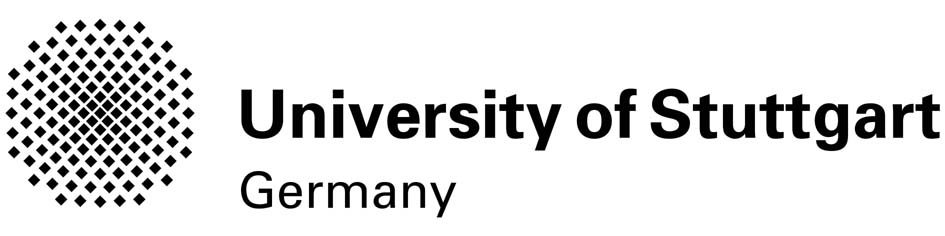
\includegraphics[width=7cm]{./Figures/unistuttgart.jpg}\\[2cm]   

{\Large Forschungsarbeit supervised by \\[.7cm]
Prof. Dr.-Ing. J. Groß \\[.4cm]
M. Sc. Wasilios Zmpitas}\\[.4cm]


{ \Large  Institut für Technische Thermodynamik, Universität Stuttgart, December 2015}


% Author and supervisor

% Unterer Teil der Seite

\end{center}


\end{titlepage}
\newpage
\newpage
\clearpage



% \tableofcontents
% \newpage
\twocolumn[
	\maketitle
  \begin{@twocolumnfalse}
    \maketitle
    \begin{abstract}
      In this work, we give an introduction to the fundamentals of graph theory. We explore M.S. Wertheim's
      multiple density formalism in analogy to the procedure of the Mayer cluster expansion.
      The parameter $\la'$ in the second order TPT approximation by Wertheim is fitted to
      simulation results to obtain more accurate approximations to simulation data than with the former
      fit. 
\\
\\
    \end{abstract}
  \end{@twocolumnfalse}
]
\section{Introduction}

This introductory article is meant to give the key ingredients to understanding M.S. Wertheim's theory, presented in
references \cite{Wertheim1}\cite{Wertheim2}\cite{Wertheim3}\cite{Wertheim4}\cite{WertheimTPT}. To that end, Section \ref{GrT}
will introduce the fundamental ideas of graph theory, which will be applied to the grand canonical partition function
to derive the \ep{Mayer Cluster Expansion} (MCE) in Section \ref{MCE}. Since Wertheim follows an analogous argumentation to the
MCE, Section \ref{WH} will simply illustrate the major variations proposed by Wertheim and explain their advantages. Section
\ref{TPT} uses \ep{Thermodynamic Perturbation Theory} (TPT) to yield approximations to compressibility values. These results are
compared and fitted to simulation results. Section \ref{Con} gives concluding remarks and an outlook.


\section{Graph Theory}
\label{GrT}
\subsection{Basic Definitions}
Fundamental to everything that follows is the basic notion of a graph. This
section shall give a definition of various common elements of graphs and
mention three important lemmas that are often used in graph theory. To simplify
the application in the following sections, we will use physically interpreable
function names. However, the theory is purely mathematical and does not require
any physical argumentation by itself.

The basic notion of a graph is described in a first definition.

\begin{defi}
\label{graphdefi_1}
Let $\r \in \Om$ with a domain $\Om \sus \R^d$. Let ${z_i : \Om \mapsto \R}$ and ${f_\mu : \Om \ti \Om \mapsto \R}$, $i, \mu \in \N$ be functions
in one and two variables, respectively. We call $z_i$ the \ep{properties} and $f_\mu$ the \ep{bonds}. With them, the following equations hold:
\begin{enumerate}[i.]
  \item A \ep{labelled point} with a property corresponds to a function in one variable:
   \begin{equation}
  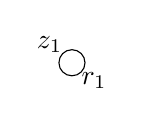
\begin{tikzpicture}[baseline={(current bounding box.center)}]%current bounding box.center
  	\draw (1,0) node[circle,minimum size=0.2cm,draw] (A) {};
	\node [above left] at (A) {$z_1$};
  	\node [below right] at (A) {$\r_1$};
	\end{tikzpicture}
= z_1(\r_1).
\end{equation}
  \item Two labelled points with a bond correspond to a function in two variables:
  \begin{equation}
  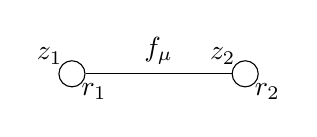
\begin{tikzpicture}[baseline={(current bounding box.center)}]%current bounding box.center
  \draw (1.0,0) node[circle,minimum size=0.2cm,draw,baseline=center] (A) {};
  \draw (3.2,0) node[circle,minimum size=0.2cm,draw] (B) {};

  \node [above left] at (A) {$z_1$};
  \node [below right] at (A) {$\r_1$};

  \node [above left] at (B) {$z_2$};
  \node [below right] at (B) {$\r_2$};


  \draw (A.east) -- node[above]{$f_\mu$} (B.west);
\end{tikzpicture}
= z_1(\r_1) f_\mu(\r_1,\r_2) z_2(\r_2).
\end{equation}
  \item This can be generalized as \\
  \{A graph with $n$ labelled points and $K$ bonds with\\*
  \vphantom{}\hskip5pt  $m(\mu,ij)$ bonds of type $\mu$ connecting points $i$ and $j$\}\\
    \itemEq{\begin{aligned}
  \qquad= \prod_{i=1}^n z_i(\r_i) \prod_{j>i}^n \prod_{\mu=1}^K\frac 1 {m(\mu,ij)!} f_\mu(\r_i,\r_j)^{m(\mu,ij)}.
  \label{fulldefi1}
  \end{aligned}}
  %\begin{flalign}
  %\begin{aligned}
  %\{\te{A graph with } n \te{ labelled points and } K \te{ bonds with }\\
  %m(\mu,ij) \te{bonds of type }\mu\te{ connecting points } i\te{ and }j\} \\
 % \qquad = \prod_{i=1}^n z_i(\r_i) \prod_{i>j}^n \prod_{\mu=1}^K\frac 1 {m(\mu,ij)!} f_\mu(\r_i,\r_j)^{m(\mu,ij)}.
  %\end{aligned}
 % \end{flalign}
\end{enumerate}
\end{defi}

A quick remark on the last item of the definition: if there is no bond of type $\mu$ present between
points $i$ and $j$, $m(\mu,ij)$ will be zero and the contribution of the bond-term in the product will
be one. For all application we will discuss in this article, $m(\mu,ij)$ will
be one or zero. Some authors, including for example Stell \cite{Stell}, call such
graphs were not more than one bond between two particles is allowed \ep{simple
graphs}. Since we will only meet such simple graphs, we keep the nomenclature
short by just calling them graphs.

As a first advantage of graph theory, we can see that large products of functions can be simplified
by replacing them with rather simple drawings. The true power within this ansatz is the easy
manipulation of complicated (sums of) functions by set theoretic
or topological considerations on graphs.

Note that the label of a labelled point is not the property $z_i$ but the fact
that a fixed variable $\bo r$ is assigned to that point. For brevity, the names
of properties, labels or bonds can be omitted when it is clear from the
context. Sometimes different graphical representations are used to distinguish
between bond types or properties.

The next definition introduces integration into graph theory.

\begin{defi}
\label{graphdefi_2}
A \ep{field point} is a filled point (usually without a label) and means integration over the coordinate:
\begin{enumerate}[i.]
  \item \itemEq{
  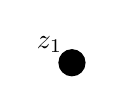
\begin{tikzpicture}[baseline={([yshift=-.7em]current bounding box.center)}]%current bounding box.center
  	\fp{(0,0)}A
	\node [above left] at (A) {$z_1$};
	\end{tikzpicture}
= \int_\Om \dr_1\ z_1(\r_1) .
  }
  \item
  \itemEq{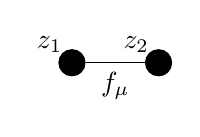
\begin{tikzpicture}[baseline={(current bounding box.center)}]%current
  % bounding box.center
  	\fp{(0,0)} A
  	\fp{(1.1,0)} B
  	\draw (A.east) -- node[below]{$f_\mu$} (B.west);
	\node [above left] at (A) {$z_1$};
	\node [above left] at (B) {$z_2$};
	\end{tikzpicture}= \int_\Om \dr_2 \int_\Om \dr_1 z_1(\r_1) f_\mu(\r_1,\r_2)
z_2(\r_2).
\label{2fields}}
%	\vskip-.5cm

 \item And the general version:%\vskip5pt%\newline
   \begin{equation}
   \begin{aligned}
  &\te{\{A graph with $n$ labelled points and $m$ field points}\\
  &\ph\{\te{and arbirtrary bonds\}}\\
  &= \int_\Om \dr_{n+m} \cdots
  \int_\Om \dr_{n+1} \times \{\te{the same graph with }\\
  &\qquad\te{all field points carrying label $\r_{n+1}$ to $\r_{n+m}$}\}.
  \label{fielddefinition}
  \end{aligned}
   \end{equation}

\end{enumerate}
\end{defi}

With graphs, the interdependences of integration variables are clearly visible.
This helps to easily detect \ep{steric incompatibilities}, e.g. graphs vanishing
because their geometry always results in a value of zero. In the hard spheres case
we will study, this is always due to overlapping spheres.

The variables $\r_1,\ldots,\r_N$ are often abbreviated by $1,\ldots,N$. This is
also done if the orientations $\Om_1,\ldots,\Om_N$ of the particles play an
important role (i.e. if they are non-spherical), where the variable $i$ then
contains both $\r_i$ and $\Om_i$.

\subsection{Graph Symmetry}
\label{GraphSym}

With the above definition, labels of field points can be set arbitrarily or omitted entirely,
all resulting in the same graph. This is in agreement with the mathematical intuition that
integration variables can be named arbitrarily as long as they stay well-defined and
distinguishable. However, we will see in Section \ref{MCE} that when using graphs to
analyze the grand canonical ensemble, the prefactors of the arising graphs play an important
role. Therefore, some authors (e.g. Morita \& Hiroike in their definitions $3$ and $3'$ \cite{MoritaHiroike})
use a definition that distinguishes between graphs with labelled field points and graphs with unlabelled
field points. We will also give this definition for completeness, but note that we will not stick to it.
For a deeper understanding, we will consider the graph
\newcommand\exgraph[3]{
  \draw(0,0) node[circle,minimum size=.2cm,draw,fill=black] (A) {};
  \draw(1.3,0) node[circle,minimum size=.2cm,draw,fill=black] (B) {};
  \draw(.65,1) node[circle,minimum size=.2cm,draw,fill=black] (C) {};
  \draw (A.center) -- (B.center);
  \node [below right] at (A) {#1};
  \node [below right] at (B) {#2};
  \node [below right] at (C) {#3};
  }
  \begin{equation}
\begin{tikzpicture}[baseline={(current bounding box.center)}]
  \exgraph{}{}{}
\end{tikzpicture} \ \ :=\ \ 
\begin{tikzpicture}[baseline={(current bounding box.center)}]
  \exgraph{}{}{}
  \node at (.65,-.25) {$f$};
  \node [above left] at (A) {$z$};
  \node [above left] at (B) {$z$};
  \node [above left] at (C) {$z$};
\end{tikzpicture}.
\label{GraphSym:Fundamental}
\end{equation}
We will use the shorthand form on the left hand side of \eqref{GraphSym:Fundamental} to
keep the overview. Obviously, as long as we label the field points in a
distinguishable manner, their labels are arbitrary and only serve as dummy names
for the integration process.
It is, however, convenient to introduce an equivalency relation between
two graphs with labelled points and field points carrying labels: two graphs are
\ep{topologically indistinguishable} if points with the same label $i$ carry the same properties and pairs of points with
labels $i$ and $j$ are linked by the same bonds in both graphs. For example,

\begin{equation}
\begin{tikzpicture}[baseline={(current bounding box.center)}]
  \exgraph{1}{2}{3}
\end{tikzpicture}
\cong
\begin{tikzpicture}[baseline={(current bounding box.center)}]
  \exgraph{2}{1}{3}
\end{tikzpicture}.
\label{equivalent graph}
\end{equation}
where the $\cong$ sign means topological indistinguishability. Conversely, two graphs are 
topologically distinguishable -- indicated here by the $\ncong$ sign -- if the bonds or
properties assigned to their points differ, as in 
\begin{equation}
\begin{tikzpicture}[baseline={(current bounding box.center)}]
  \exgraph{1}{2}{3}
  \end{tikzpicture}
\ncong
\begin{tikzpicture}[baseline={(current bounding box.center)}]
  \exgraph{1}{3}{2}
\end{tikzpicture},
\label{not equivalent graph}
\end{equation}

The numerical value represented by all graphs in \eqref{equivalent graph} and 
\eqref{not equivalent graph} is the same, and we did already note above that from a
mathematical point of view the labelling of the integration variables
is of no importance. So why is this distinction necessary at all?

There are multiple answers to that question. First of all, there is no unique
way to transform some expression containing properties, bonds and integrals into
a graph. Mathematically, the expressions
\begin{equation}
\begin{tikzpicture}[baseline={(current bounding box.center)}]
\exgraph{1}{2}{3}
\end{tikzpicture}
\cong
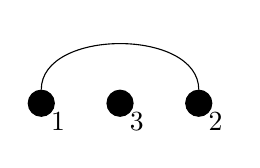
\begin{tikzpicture}[baseline={(current bounding box.center)}]
\fp{(0,0)} A
\fp{(1,0)} B
\fp{(2,0)} C
\foreach \x/\y in {A/1,B/3,C/2} {\node [below right] at (\x) {\y};}
\draw    (A) to[out=90,in=90] (C);
\end{tikzpicture}
\end{equation}
represent the exact same object. This is a first reason to know which graphs
are actually the same even if they may appear to be different at first glance.

Another answer to this question lies in the application of graph theory to
problems of physics. When applying graph theory to the grand canonical partition function in Section \ref{MCE},
we will encounter sums over graphs. These will only contain topologically distinguishable
graphs, and a graph of $N$ points will be weighted by a factor of $(N!)\iv$. When only considering
the graphs in the example above, the sum will contain the expression
\begin{equation}
\begin{aligned}
\frac 1 {6} 
&\lt\{
\begin{tikzpicture}[baseline={(current bounding box.center)}]
  \exgraph{1}{2}{3}
\end{tikzpicture}
\rt.+\lt.
\begin{tikzpicture}[baseline={(current bounding box.center)}]
  \exgraph{3}{1}{2}
\end{tikzpicture}
+
\begin{tikzpicture}[baseline={(current bounding box.center)}]
  \exgraph{2}{3}{1}
\end{tikzpicture}
\rt\}\\
&=\frac 1 2 \lt\{
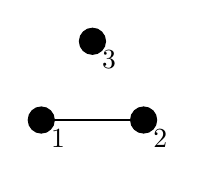
\begin{tikzpicture}[baseline={(current bounding box.center)}]
  \draw(0,0) node[circle,minimum size=.2cm,draw,fill=black] (A) {};
  \draw(1.3,0) node[circle,minimum size=.2cm,draw,fill=black] (B) {};
  \draw(.65,1) node[circle,minimum size=.2cm,draw,fill=black] (C) {};
  \draw (A.center) -- (B.center);
  %\node [above left] at (A) {$z$};
  %\node [above left] at (B) {$z$};
  %\node [above left] at (C) {$z$};
  \node [below right] at (A) {1};
  \node [below right] at (B) {2};
  \node [below right] at (C) {3};
\end{tikzpicture}\rt\}.
\end{aligned}
\label{GraphSym:Bigsum}
\end{equation}
The left hand side of \eqref{GraphSym:Bigsum} can be shortened to a single
expression because the values of all graphs on the left hand side are the same. The factor
$\frac 1 2$ is an important property of the graph \eqref{GraphSym:Fundamental}. It is the
inverse of the \ep{symmetry number} $s$. The symmetry number is given by the number
of permutations of graph labels that lead to topologically indistinguishable graphs.
In our example, this number is $2$ according to \eqref{equivalent graph}. It is easily verified that
the factor $(N!)\iv$ always reduces to $s\iv$: Assigning labels from $1$ to $N$ to the $N$ field points
of a graph leads to $N!$ graphs. For every type of topologically distinguishable
graphs there are $s$ topologically indistinguishable versions. Omitting all
but one of these leads to a total of $\frac {N!} s$ topologically
distinguishable graphs.
These all have the same value, so if we sum over them and divide by $N!$, we
can choose any label assignment and multiply it by
$\frac 1 {N!} \frac {N!} s = \frac 1 s$.

The symmetry number is an important property of a graph. Some authors include it
directly in the basic definition of a graph, thereby distinguishing between
graphs with labelled field points and graphs with unlabelled field points. We will
not do so, which leads to different equations. 

\subsection{Derivatives of Graphs}

While integration by definition turns a labelled point into a field point, turning
a field point back into a labelled point requires a slight bit of analysis. For that purpose,
we introduce the variational calculus, and thereby differentiation, into the graph theoretic framework.

%% CHECK: Really functional derivative? Not just the variation?
\renewcommand\zi{z}
\renewcommand\zip{z'}
\begin{defi}
\label{funcderivative}
Let $\zi$ be defined as in Defintion \ref{graphdefi_1} and let $\La: \zi \mapsto \R$ be a functional.
Then the \ep{functional derivative} \sdelti \La {\zi} is defined via the \ep{variation} $\dl\La$ of $\La$
and $\dl \zi$ of $\zi$ by
\begin{equation}
\dl\La = \int \drr \delti\La {\zi(\r)}\ \dl\zi(\r)
\label{FuncDeri}
\end{equation}
\end{defi}

Integration over the label of a labelled point is of course a functional of the property assigned
to that labelled point (and the bonds adjacent to it, but we will not use that
here). It is therefore an excellent candidate to use the above definition. We
will use the relationship
\begin{align}
\label{difrelation}
\delti{\zi(\r)}{\zip(\r')} =
\begin{cases}
0 & \te{for }\zi\te{ independent of }\zip,\\
\dl(\r - \r') & \te{for }\zi\equiv \zip.
\end{cases}
\end{align}

We can use that on the situation given in equation \eqref{2fields} for
$\zi\equiv\zip\equiv z$ and generalize the results found there:
\begin{equation} %CHECK: Ableitungen in Variationsrechnung
\begin{aligned}
&\hspace{-.7cm}\delti{}{z(\r)}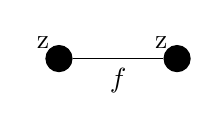
\begin{tikzpicture}[baseline={(current bounding
box.center)}]%current bounding box.center
  	\draw (0,0) node[circle,minimum size=0.2cm,draw,fill=black] (A) {};
  	\draw (1.5,0) node[circle,minimum size=0.2cm,draw,fill=black,align=center] (B) {};
  	\draw (A.east) -- node[below]{$f$} (B.west);
	\node [above left] at (A) {z};
	\node [above left] at (B) {z};
	\end{tikzpicture}\\
	&= \int \dr' \int \dr'' \delti{}{z(\r)} \lt[z(\r') f(\r',\r'') z(\r'')\rt]\\
&= \int \dr' \int \dr'' \lt[\dl(\r-\r') f(\r',\r'') z(\r'')\rt] \\
	&\qquad + \int \dr' \int \dr'' \dl(\r-\r'') f(\r',\r'') z(\r') \\
	&= 2 \int \dr' f(\r,\r') z(\r') \\
    &=2 \ \ \ 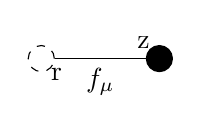
\begin{tikzpicture}[baseline={(current bounding box.center)}]%current bounding box.center
  	\draw (0,0) node[circle,minimum size=0.2cm,dashed,draw] (A) {};
  	\draw (1.5,0) node[circle,minimum size=0.2cm,draw,fill=black] (B) {};
  	\draw (A.east) -- node[below]{$f_\mu$} (B.west);
	\node [above left] at (B) {z};
	\node [below right] at (A) {\r};
	\end{tikzpicture}.
	\label{funcderi:ex}
\end{aligned}
\end{equation}

The dashed lines around the left point indicate that there is no property assigned to it.
Thus, the functional derivative of a graph is identical to turning field points
into labelled points. One can easily explain this in a straightforward way: the functional
derivative of a graph $\Ga$ with respect to a property $z(\r)$ is equal to the sum of all graphs obtained
from $\Ga$ by turning a single field point with property $z$ into a point labelled $\r$, and the
point loses its property (or rather, adopts the new property $z^* \equiv 1$).

But as is the case in equation \eqref{funcderi:ex}, this would result in summing many graphs with equal value.
This redundancy stems from the aforementioned fact that our Definition \ref{graphdefi_2} has no special
treatment of graph symmetry. The derivative changes the symmetry number of the graph from $2$ to $1$. Devision
by symmetry numbers yields a useful lemma, which we will give without a prove.

% To do
% so, we start consider \emph{topologically indistinguishable} graphs: if one appends clear labels $\ri$ and $\rip$
% to field points as in \eqref{fielddefinition}, then two graphs with the same properties and bonds
% are called topologically indistinguishable if writing the graph as a functional as in \eqref{fulldefi1} leads
% to the same expression for $\ri$ and $\rip$. That is, points with the same label $i$ and $i'$ carry the same
% properties and pairs of points with labels $i$ and $j$ are linked by the same bonds as points $i'$ and $j'$
% CHECK: Das stimmt nur teilweise! Die beiden Graphen oben sind ja nicht identisch, wenn man die Indize vertauscht.
% These graphs are called \emph{topologically indistinguishable}: two graphs are topologically indistinguishable if the fully
% spelled equation according to \eqref{fulldefi1} reads the same for both, that is properties and bonds are
% unchanged with repect to variable labels \ri.
% CHECK: Needs to be supervised! Topologically distinguishable ist nicht richtig so weit.
% It would be easier to just sum over all topologically distinugishable
%  graphs and multiplying each of these by the number of times they appear in the sum. This number is the \ep{symmetry number s}
%  of a graph. It is equal to the number of topologically indistinguishable permutations
%  of graph labels on field points, and in the simple example of equation \eqref{funcderi:ex} it is clear that
%  this number is 2.
%
% Some authors, like Hiroike and Morita \cite{MoritaHiroike}, include it in the
% definition of a graph, multiplying the right hand side of equation \eqref{fielddefinition} by $\frac 1 s$.
% Despite advantages especially in dealing with functional derivatives (the factor 1 on the left
% hand side of equation \eqref{funcderi:ex} would lead to a factor $\frac 1 2$ in the following
% equations, eliminating the factor 2 coming from the derivation), we chose the alternative
% version of not including the symmetry number in order to maintain the equality
% \begin{equation}
% \begin{tikzpicture}[baseline={(current bounding box.center)}]%current bounding box.center
%   	\draw (0,0) node[circle,minimum size=0.2cm,draw,fill=black] (A) {};
%   	\draw (1.5,0) node[circle,minimum size=0.2cm,draw,fill=black] (B) {};
%   	\draw (A.east) -- node[below]{$f$} (B.west);
% 	\node [above left] at (A) {$z_1$};
% 	\node [above left] at (B) {$z_2$};
% 	\node [below right] at (A) {$\r_1$};
% 	\node [below right] at (B) {$\r_2$};
% 	\end{tikzpicture}
% 	=
% \begin{tikzpicture}[baseline={(current bounding box.center)}]%current bounding box.center
%   	\draw (0,0) node[circle,minimum size=0.2cm,draw,fill=black] (A) {};
%   	\draw (1.5,0) node[circle,minimum size=0.2cm,draw,fill=black] (B) {};
%   	\draw (A.east) -- node[below]{$f$} (B.west);
% 	\node [above left] at (A) {$z_1$};
% 	\node [above left] at (B) {$z_2$};
% 	\end{tikzpicture},
% \end{equation}
% which does not distinguish between graphs with clearly named integration variables and such
% without. This is in agreement with the definitions of the graph theory Wertheim \cite{Wertheim1} uses.

%In conclusion, we give the following Lemma without a prove:

\begin{lem}
Let $\zi$, $\zip$ be properties and let $\Ga$ be a graph and let the set
$\st{\Ga_\al(\r)}_{1\le\al\le m}$ be the set of all topologically
distinguishable graphs obtainable from $\Ga$ by turning one field point with
property $\zi$ into a labelled point depending on $\r$ with property $\zip$. Let
$s$ be the symmetry number of $\Ga$ and let the set $\st{s_\al}_{1\le\al\le m}$
be the set of symmetry numbers corresponding to $\st{\Ga_\al(\r)}$. Then
\begin{equation}
\zip(\r)\delti{}{\zi(\r)} s\iv\ \Ga = \sum_{\al=1}^m s_\al\iv\ \Ga_\al(\r).
\end{equation}
\label{funcderi2}
\end{lem}
Of course, if $\Ga$ has no $\zi$ field points, the derivative amounts to
zero as does the sum over the empty set on the right hand side. Note again that
Lemma \ref{funcderi2} would look differently if all graphs already contained division by symmetry number.

\subsection{Articulation Points}
\label{ArtPoint}

Most considerations on graphs take only the topology of a graph into account. From the
topology, it is possible to derive reductions which can ultimately result in
huge simplifications of originally very complicated expressions.
%And since the topology
%of a graph can be analysed with relative ease, the simplifications can often be
%seen and communicated without tedious considerations of integration variables.

For example, finding independent integration variables can be easily translated to a topological consideration.
That is this subsection's purpose, and we will only need a short list of definitions
to get there. The following properties are relevant in graph theory:

\begin{itemize}
  \item \ep{connected graph}: a graph $\Ga$ with two or more points is connected if for any points
  $A, B \in \Ga$ there is a path of points and bonds connecting $A$ to $B$.
  \item \ep{doubly, triply, \ldots $n$-connected graph}: a graph $\Ga$ with $n$
  or more points is $n$-connected if for any points $A, B \in \Ga$ there are $n$
  independent paths of points and bonds connecting $A$ to $B$.
%  \item \ep{single-bonded graph}: a single-bonded graph is a graph $\Ga$ where
%  no double-bonds exist between points $A, B \in \Ga$. Unconnected points are
  % allowed.
%  \item \ep{singly connected graph}: a single-bonded connected graph.
  \item \ep{articulation point}: a point $A$ in a connected graph $\Ga$. If one removes
  $A$ and its adjacent bonds, the graph $\Ga$ will be divided into two or more separate graphs.
  \item \ep{reducible graph}: a graph that contains articulation points or bonds that may be
  expressed in a more convenient way.
\end{itemize}

While these names are frequently used in graph theory, they may be understood differently in each context.
For example, the vague definition of a reducible graph comes from the fact that it is up to the
researcher which bonds they want to consider as fundemental for their graph.
%There are often multiple layers of reducibility, for example one can first
%remove all labelled articulation points and later all field articulation
%points.
As one can see especially in the paper Wertheim III\cite{Wertheim3}, the
correct definition in this matter is crucial to the types of graphs one ends up
analyzing. Wertheim III also shows that careful characterizations of
articulation points are fundamental to researches in graph theory.

Now, let us return to independent integration variables. Their treatment is
easiest understood in a simple exemplatory calculation considering a three
point singly connected graph. For simplicity, we will consider all properties
to be $z$ and all bonds to be $f$.

\begin{align}
\begin{aligned}
%&\qquad\qquad\qquad\begin{tikzpicture}[baseline={(current bounding box.center)}]%current bounding box.center
%  	\draw (0,-.5) node[circle,minimum size=0.2cm,draw,fill=white, fill opacity=0] (A) {};
%  	\draw (-.5,.5) node[circle,minimum size=0.2cm,draw,fill=black] (B) {};
%  	\draw (.5,.5) node[circle,minimum size=0.2cm,draw,fill=black] (C) {};
%  	\draw (A.north west) --  (B.center);
%  	\draw (A.north east) --  (C.center);
%  	\node [below right] at (A) {\r};
%\end{tikzpicture} \\
&\qquad\qquad\qquad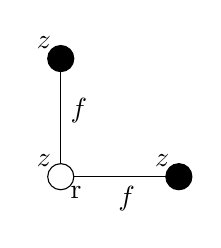
\begin{tikzpicture}[baseline={(current bounding box.center)}]%current bounding box.center
  	\draw (0,0) node[circle,minimum size=0.2cm,draw,fill=white, fill opacity=0] (A) {};
  	\draw (0,1.5) node[circle,minimum size=0.2cm,draw,fill=black] (B) {};
  	\draw (1.5,0) node[circle,minimum size=0.2cm,draw,fill=black] (C) {};
  	\draw (A.north) --  node[right]{$f$}(B.center);
  	\draw (A.east) --  node[below]{$f$}(C.center);
  	\node [above left] at (A) {$z$};
	\node [above left] at (B) {$z$};
	\node [above left] at (C) {$z$};
  	\node [below right] at (A) {\r};
\end{tikzpicture} \\
&= \int_\Om \dr'\ \int_\Om \dr''\ z(\r) z(\r') z(\r'') f(\r,\r') f(\r,\r'') \\
&= z(\r) \int_\Om \dr'\ \int_\Om \dr''\ z(\r') f(\r,\r') z(\r'') f(\r,\r'') \\
&= z(\r) \brc{\int_\Om \dr'\  z(\r') f(\r,\r')} \\
&\qquad\times \brc{\int_\Om \dr''\ z(\r'') f(\r,\r'')} \\
%&= z(\r) \brc{\int_\Om \drr'  z(\r') f(\r,\r')}^2 \\
&=\qquad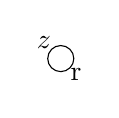
\begin{tikzpicture}[baseline={(current bounding box.center)}]%current bounding box.center
  	\draw (0,0) node[circle,minimum size=0.2cm,draw,fill=white, fill opacity=0] (A) {};
  	\node [below right] at (A) {\r};
  	\node [above left] at (A) {$z$};
\end{tikzpicture}
\times \
\brc{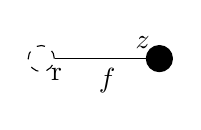
\begin{tikzpicture}[baseline={(current bounding box.center)}]%current bounding box.center
  	\draw (0,0) node[circle,minimum size=0.2cm,draw,fill=white,dashed] (A) {};
  	\draw (1.5,0) node[circle,minimum size=0.2cm,draw,fill=black] (B) {};
  	%\draw (.1,-.3) --  (B.center);
  	\node [above left] at (B) {$z$};
  	\draw (A.east) --  node[below]{$f$}(B.center);
  	\node [below right] at (A) {\r};
\end{tikzpicture}}^2.
\end{aligned}
\label{articul:ex}
\end{align}
This simple example can be used to illuminate a few ideas. First of all, we used the
independence of integration variables in line 3 to reach line 4. On the other hand, the original graph
and the resulting graph can be linked with the following procedure if we consider that the
labelled point is an articulation point: Separate the graph at the articulation point. Each
of the resulting graphs may be computed with the articulation point replaced by a point
without properties but with the same label as the labelled point. The original
graph is the product of all graphs resulting from the separation times the articulation
point with the corresponding property.

Another idea underlying the transformation in equation \eqref{articul:ex} is the fact that
identifying independent subgraphs -- independent in a sense that they are only linked by
articultion points -- can simplify graph computation.

A third remark concerns what simplifications may be made after arriving at the right hand side
of equation \eqref{articul:ex}. We did already reduce the number of integrations to be carried
out. But we could also go further and define a new property according to
\begin{equation}
z^*(\r) := z(\r) \times
\brc{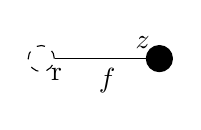
\begin{tikzpicture}[baseline={(current bounding box.center)}]%current bounding box.center
  	\draw (0,0) node[circle,minimum size=0.2cm,draw,fill=white,dashed] (A) {};
  	\draw (1.5,0) node[circle,minimum size=0.2cm,draw,fill=black] (B) {};
  	%\draw (.1,-.3) --  (B.center);
  	\node [above left] at (B) {$z$};
  	\draw (A.east) --  node[below]{$f$}(B.center);
  	\node [below right] at (A) {\r};
\end{tikzpicture}}^2,
\end{equation}
reducing the full graph altogether to

\begin{equation}
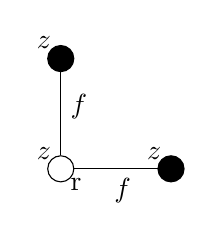
\begin{tikzpicture}[baseline={(current bounding box.center)}]%current bounding box.center
  	\draw (0,-.7) node[circle,minimum size=0.2cm,draw,fill=white, fill opacity=0] (A) {};
  	\draw (0,.7) node[circle,minimum size=0.2cm,draw,fill=black] (B) {};
  	\draw (1.4,-.7) node[circle,minimum size=0.2cm,draw,fill=black] (C) {};
  	\draw (A.north) --  node[right]{$f$}(B.center);
  	\draw (A.east) --  node[below]{$f$}(C.center);
  	\node [above left] at (A) {$z$};
	\node [above left] at (B) {$z$};
	\node [above left] at (C) {$z$};
  	\node [below right] at (A) {\r};
\end{tikzpicture}
\ \  = \ \ 
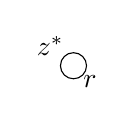
\begin{tikzpicture}[baseline=0]%current bounding box.center
  	\draw (0,0) node[circle,minimum size=0.2cm,draw,fill=white, fill opacity=0] (A) {};
  	\node [above left] at (A) {$z^*$};
  	\node [below right] at (A) {$\r$};
\end{tikzpicture}.
\label{articul:simple}
\end{equation}
Systematically used, this simple trick is again capable of reducing large graphs in a
straightforward way, and we will in fact use it in the Mayer cluster expansion.

In the above example, the articulation point was a labelled point. We chose this
setting to clearly show the $\r$-dependence in the reduced graphs. Of course, the same
formalism can be used on a field articulation point, but some care has to be taken
when treating the integration variable of the field point. If one turned all labelled
points in equation \eqref{articul:simple} into field points, the equality would still hold,
while when turning all labelled points in equation \eqref{articul:ex} into field points,
the expressions would not necessarily be equal.

\subsection{Exponentials of Graphs}
At the end of this section, we give two very powerful lemmas which are crucial for many
applications of graph theory. A proof can be found in Morita and Hiroike \cite{MoritaHiroike} (Lemmas 3 and 4),
we will just give the basic idea behind it. The first lemma is

\begin{lem}
\label{lemma:exponential}
% CHECK: Für field points funktioniert es auf jeden Fall. Es müsste aber auch für labelled
%     points klappen, dann müsste man sich nochmal überlegen, wie M und N aussehen.
%     Man muss sich auch überlegen, wie die Symmetriezahlen einbezogen werden.
% CHECK: topologically distinguishable? Wie sind die Graphen unterscheidbar/unterschiedlich?
Consider two sets of graphs of field points, $A:=\st{\Ga_\al}$ and $B:=\st{\La_\be}$,
with corresponding sets of symmetry numbers $\st{s_\al}$ and $\st{\tilde s_\be}$.
Let $B$ contain all connected subgraphs of $A$ and the single field point graph. If any $\Ga_\al \sus A$ is
a product of graphs $\La_\be \sus B$ (with a graph possibly appearing multiple times or not at all), and any
product of graphs $\La_\be \sus B$ is represented by exactly one $\Ga_\al \sus A$, then
\begin{equation}
1 + \sum_{\al\ |\ \Ga_\al \in A} {s_\al}\iv\ \Ga_\al = \exp\lt(\sum_{\be\ |\ \La_\be \in B} {\tilde s_\be}\iv\ \La_\be \rt).
\label{Lemma5:eq}
\end{equation}
\end{lem}
Note that a set $A$, in order to fulfill the prerequisites of the previous lemma, has to be
infinite. This does not apply to the set $B$.

To understand Lemma \ref{lemma:exponential}, we consider the exponential function. If one does not
consider factors, the exponential function is $1$ plus a sum of all powers of the exponent.
The $1$ is already on the left hand side of \eqref{Lemma5:eq}, so only the sum remains. Since each graph in $A$ is a product of graphs in
$B$, and $A$ contains all products of graphs in $B$, summing over all graphs in $A$ must contain
the same graphs as the exponential function of a sum of all graphs in $B$. One can prove
that the sums are exactly the same if one examines the factors resulting from the symmetry
numbers and the factors $(N!)\iv$ in the exponential series.

A similar lemma which uses articulation points is
\begin{lem}
\label{lemma:articulation}
Consider two sets of connected graphs $A:=\st{\Ga_\al}$ and $B:=\st{\La_\be}$
with corresponding sets of symmetry numbers $\st{s_\al}$ and $\st{\tilde s_\be}$. The graphs in $A$ and $B$
do all contain exactly the same labelled points without property and an
arbitrary number of field points. Let $B$ contain all the subgraphs of $A$ that stay connected if the labelled
points are removed. If any $\Ga_\al \sus A$ can be uniquely decomposed into
(possibly identical) graphs belonging to $B$ by separating $\Ga_\al$ at the labelled points, and any graph obtained by joining together
(possibly identical) graphs from $B$ at the labelled points uniquely belongs to $A$, then
\begin{equation}
1 + \sum_{\al\ |\ \Ga_\al \in A} {s_\al}\iv\ \Ga_\al = \exp\lt(\sum_{\be\ |\ \La_\be \in B} {\tilde s_\be}\iv\ \La_\be \rt).
\label{Lemma6:eq}
\end{equation}
\end{lem}
The proof for this lemma is exactly the same as for Lemma \ref{lemma:exponential}, since the process of
joining together graphs at labelled points without property is again a simple graph multiplication,
so the arguments for the power series in the exponential function and the inclusion of symmetry
numbers need not be changed.  

An infinite sum of graphs can therefore be expressed by the exponential of a sum of elemental
subgraphs, which may be finite. This result will prove useful in the following sections.

\section{The Mayer Cluster Expansion}
\label{MCE}

\subsection{Fundamentals}
The MCE uses graph theory to tackle statistical mechanics. Our task is to
acquire thermodynamic properties of a system in thermal equilibrium which
contains identical particles moving in the fixed volume $V$ at the fixed
temperature $T$ and the fixed chemical potential $\mu$. The system is to be considered uniform, that is all properties have the same value throughout the entire system.
 The properties of interest may for example be the \ep{pressure} $p$
or the \ep{density} $\rho$. To that end, we consider the graph
theoretical approach to obtain a useful expression for the \ep{grand canonical partition function} $\Xi$,
\begin{equation}
\Xi(\mu,V,T)=\sum_{N\ge0} e^{N \mu/k_B T} Q(N,V,T)
\label{GrandCanonical}
\end{equation}
with %the \ep{chemical potential} $\mu$, the \ep{volume} $V$, the \ep{temperature} $T$, 
the \ep{Boltzmann constant} $k_B$
and the \ep{canonical partition function} $Q$. The sum runs over all \ep{numbers of particles} $N$ contained in $V$.
A common replacement is
\begin{equation}
\be:=\frac 1 {k_B T},
\end{equation}
and we can define the \ep{fugacity} by
\begin{equation}
\tilde z:=e^{\be \mu}.
\label{fuga.1}
\end{equation}
The canonical partition function is given by
%% CHECK: Orientation dependence? 
\begin{equation}
 \begin{aligned}
 Q(N,V,T)=\underbrace{\frac {V^N}{N!\la_\te{th}^{3N}}}_{Q^{(ig)}(N,V,T)} \frac 1 {V^N} \int \dr^N\ \exp\lt[-\be U_N(\r^N)\rt],
 %Q(N,V,T)=\frac {V^N}{N!\la_\te{th}^{3N}}\frac 1 {V^N} \int &\dr^N\di\Om^N\\
 %&\times \exp\lt[-\be U_N(\r^N,\Om^N)\rt],
% &=:Q^{\te{ig}}(N,V,T) \frac 1 {V^N} \int \dr^N\ \exp\lt[-\be U_N(\r^N)\rt].
 \end{aligned}
%Q(N,V,T)=Q^{\te{ig}}(N,V,T) \frac 1 {V^N} \int \dr^N\ \exp\lt[-\be U_N(\r^N)\rt].
\label{QNVT}
\end{equation}
with a \ep{potential} $U_N$ in which the particles move. The prefactor contains the value
of the canonical partition function of the ideal gas $Q^{(ig)}(N,V,T)$, with the \ep{thermal wavelength}
\begin{equation}
\la_\te{th}=\sqrt{\frac {h^2} {2\pi mk_BT}},
\end{equation}
where $m$ is a particle's mass and $h$ is \ep{Planck's constant}. Note that the potential $U_N$ does
not depend on particle velocity, that is the particles move in a \ep{force field}. 

%Another remark on the
%form of equation \eqref{QNVT} is the fact that it would be possible to eliminate the factor $V^N$. We do
%not do so for reasons to be explained soon.

%, dependent on the \ep{thermal wavelength} $\tilde \La$.
% CHECK: wirklich thermal wavelength? Wie viel von all den Namen sollte man droppen? Wie viele darf
% man als bekannt voraussetzen?
For all that follows, we will only consider two-body interaction potentials of the form
% \begin{equation}
% \begin{aligned}
% U_N &= \sum_{i=1}^N \sum_{j>i} \phi(ij), \\
% % \phi(ij)&=\phi_R(ij)+\\
% % &\qquad\sum_\al\sum_\be \phi_{\al\be}(\abs{\r_j+\d_\be(\Om_j)-(\r_i+\d_\al(\Om_i))}).
% \phi(ij)&=\phi_R(ij)+\sum_\al\sum_\be \phi_{\al\be}(\abs{\r_\be-\r_\al}), \\
% \phi_R(ij)&>0, \qquad
% \phi_{\al\be}<0.
% \end{aligned}
% \end{equation}
% Here, the sum over $\al$ and $\be$ runs over the \ep{interaction sites} on each particle. We also
% employed the common shorthand version $\phi(ij):=\phi(\r_i,\r_j)$. We separated the potential already
% into a purely \ep{repulsive part} $\phi_R$ and an \ep{attractive part} given by the site-site interaction
% potential $\phi_{\al\be}$.
\begin{equation}
\begin{aligned}
U_N &= \sum_{i=1}^N \sum_{j>i} \phi(ij), \\
\phi(ij)&:=\phi(\r_i,\r_j) = \phi(\r_j,\r_i).
\label{potential}
\end{aligned}
\end{equation}
For now, we do not need to know any further details on the interaction potential.
%For non-symmetric
%potentials, i.e. potentials not satisfying the second condition of \eqref{potential}, graphs would
%have to contain further information concerning the direction of the interaction.

In order to adjust the upper equations to their use in graph theory, we make a change to the definition
of the fugacity in equation \eqref{fuga.1} and give it the new form
\begin{equation}
%z:=\frac V {\lath^3} \tilde z.
z:=\frac {\tilde z} {\lath^3} .
\label{fuga.2}
\end{equation}
In all that follows, we will refer to the quantity $z$ when talking about fugacity, ignoring that
$\tilde z$ and $z$ have different dimensions. 
% and the upshot of the replacement is that we will face integrals of the form
% \begin{equation}
% \frac 1 {V^N} \int \dr^N \ldots,
% \label{int:norm}
% \end{equation}
% which are obviously very simple to treat when integrating over constant functions.
In the framework of graph theory, our points carry property functions. We will therefore treat the fugacity as a constant function
\begin{equation}
z(i):\equiv z.
\label{zconst}
\end{equation} 

We can also use the functions
\begin{equation}
\begin{aligned}
e(ij)&:=e^{-\be \phi(ij)}, \\
f(ij)&:=e(ij)-1.
\end{aligned}
\label{eijfij}
\end{equation}
These will proof helpful if we insert \eqref{potential} into the integral in \eqref{QNVT}.
Without factors, the integral then takes the form
\begin{equation}
\begin{aligned}
\int&\dr^N \exp(-\be \sum_{j>i} \phi(ij))\\
&= \int\dr^N \prod_{j>i} e(ij)
= \int\dr^N \prod_{j>i} (f(ij)+1)\\
&= \int\dr^N [\ 1+f(12)+\ldots+f(12)f(23)+\ldots\\&\qquad\qquad+f(12)f(23)f(34)+\ldots\ ].
\end{aligned}
\label{int:etof}
\end{equation}
So, we have our functions $f(ij)$ and $z(i)$. Using all reformulations of this chapter, we can
start from equation \eqref{GrandCanonical} to reach a simplified expression
\begin{equation}
\begin{aligned}
\Xi&=\sum_{N\ge0}\tilde z^N Q(N,V,T) \\
&=\sum_{N\ge0} \frac{\tilde z^N V^N}{N!\lath^{3N}} \frac 1 {V^N}\int \dr^N \exp(-\be \sum_{j>i} \phi(ij))\\
&=\sum_{N\ge0} \frac {z^N}{N!} \int\dr^N \prod_{j>i} (f(ij)+1)\\
&=\sum_{N\ge0}\frac 1 {N!} \int\dr^N z(1)\cdots z(N)\lt[1+f(12)+\ldots\rt].
\end{aligned}
\label{Grand:simple}
\end{equation}
This sum still contains many graphs of equal value. These can be removed by arguments outlined
in Section \ref{GraphSym}. We drop the labels and include symmetry numbers for
every graph in \eqref{Grand:simple}. It is therefore possible to express $\Xi$ in terms of graphs according to

\newcommand\gbox{\makebox[1.05cm][c]} % GRAPH BOX
\newcommand\fgbox{\ph{\frac 1 2}\gbox} % GRAPH BOX with fraction
\newcommand\twofp{
\fp{(0,0)}{A}
\fp{(.7,0)}{B}
}
\newcommand\threefp{
\fp{(0,0)}{A}
\fp{(.7,0)}{B}
\fp{(.35,.7)}{C}
}
\begin{align}%{5}
\begin{aligned}
\Xi=&\ph{\frac 1 2}\gbox{1}+
\ph{\frac 1 2}\gbox{
\begin{tikzpicture}[baseline={([yshift=-.3em]current
bounding box.center)}]
  \fp{(0,0)}{A}
\end{tikzpicture}}
+
\frac 1 2
\begin{tikzpicture}[baseline={([yshift=-.3em]current bounding box.center)}]
  \twofp
\end{tikzpicture}
+
\frac 1 2
\begin{tikzpicture}[baseline={([yshift=-.3em]current bounding box.center)}]
  \twofp
  \connect{A/B};
\end{tikzpicture}&
\\
+&\frac 1 6
\begin{tikzpicture}[baseline={([yshift=-.3em]current bounding box.center)}]
  \threefp
\end{tikzpicture}
+\frac 1 2
\begin{tikzpicture}[baseline={([yshift=-.3em]current bounding box.center)}]
  \threefp
  \connect{A/B}
\end{tikzpicture}
+\frac 1 2
\begin{tikzpicture}[baseline={([yshift=-.3em]current bounding box.center)}]
  \threefp
  \connect{A/B,A/C}
\end{tikzpicture}
+\frac 1 6
\begin{tikzpicture}[baseline={([yshift=-.3em]current bounding box.center)}]
    \threefp
  \connect{A/B,A/C,B/C}
\end{tikzpicture}&
\\
+& \ldots 
\end{aligned}
\label{Grand:long}
\end{align}

We can now go on to use the results of the previous section to further simplify the
sum given here. To do so, we have a closer look at \eqref{Grand:long}. It has the form of
a sum over sums of $N$-point graphs. Each sum of $N$-point graphs contains the unconnected $N$-point
graph, a graph with $1$ connection, graphs with $2$ connections, \ldots, a graph connecting all $N$ points.
All of them are weighted with the corresponding symmetry number. For $N \ge 2$, these graphs are not all
connected. But they can all be constructed by combining connected subgraphs. On closer examination, it appears that
this does exactly amount to the prerequisite of Lemma \ref{lemma:exponential}, where the set $B$ is the
set of all connected graphs with $N \ge 1$. Using \eqref{Lemma5:eq} on \eqref{Grand:long} yields
\begin{equation}
\begin{aligned}
\ln \Xi&=
\ph{.}
\begin{tikzpicture}[baseline={([yshift=-.3em]current
bounding box.center)}]
  \fp{(0,0)}{A}
\end{tikzpicture}
+
\frac 1 2
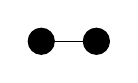
\begin{tikzpicture}[baseline={([yshift=-.3em]current bounding box.center)}]
  \draw(0,0) node[circle,minimum size=.2cm,draw,fill=black] (A) {};
  \draw(.7,0) node[circle,minimum size=.2cm,draw,fill=black] (B) {};
  \draw (A.center) --  (B.center);
\end{tikzpicture}
+\frac 1 2
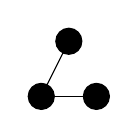
\begin{tikzpicture}[baseline={([yshift=-.3em]current bounding box.center)}]
  \draw(0,0) node[circle,minimum size=.2cm,draw,fill=black] (A) {};
  \draw(.7,0) node[circle,minimum size=.2cm,draw,fill=black] (B) {};
  \draw(.35,.7) node[circle,minimum size=.2cm,draw,fill=black] (C) {};
  \draw (A.center) --  (B.center);
  \draw (A.center) --  (C.center);
\end{tikzpicture}
+
\frac 1 6
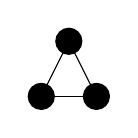
\begin{tikzpicture}[baseline={([yshift=-.3em]current bounding box.center)}]
  \draw(0,0) node[circle,minimum size=.2cm,draw,fill=black] (A) {};
  \draw(.7,0) node[circle,minimum size=.2cm,draw,fill=black] (B) {};
  \draw(.35,.7) node[circle,minimum size=.2cm,draw,fill=black] (C) {};
  \draw (A.center) --  (B.center);
  \draw (A.center) --  (C.center);
  \draw (B.center) --  (C.center);
\end{tikzpicture}
 + \ldots .
%\\
% \Xi=\exp\lt[
% \begin{tikzpicture}[baseline={([yshift=-.3em]current bounding box.center)}]
%   \draw(0,0) node[circle,minimum size=.2cm,draw,fill=black] (A) {};
% \end{tikzpicture}
% +
% \frac 1 2
% \begin{tikzpicture}[baseline={([yshift=-.3em]current bounding box.center)}]
%   \draw(0,0) node[circle,minimum size=.2cm,draw,fill=black] (A) {};
%   \draw(.7,0) node[circle,minimum size=.2cm,draw,fill=black] (B) {};
%   \draw (A.center) --  (B.center);
% \end{tikzpicture}
% +\frac 1 2
% \begin{tikzpicture}[baseline={([yshift=-.3em]current bounding box.center)}]
%   \draw(0,0) node[circle,minimum size=.2cm,draw,fill=black] (A) {};
%   \draw(.7,0) node[circle,minimum size=.2cm,draw,fill=black] (B) {};
%   \draw(.35,.7) node[circle,minimum size=.2cm,draw,fill=black] (C) {};
%   \draw (A.center) --  (B.center);
%   \draw (A.center) --  (C.center);
% \end{tikzpicture}
% +
% \frac 1 6
% \begin{tikzpicture}[baseline={([yshift=-.3em]current bounding box.center)}]
%   \draw(0,0) node[circle,minimum size=.2cm,draw,fill=black] (A) {};
%   \draw(.7,0) node[circle,minimum size=.2cm,draw,fill=black] (B) {};
%   \draw(.35,.7) node[circle,minimum size=.2cm,draw,fill=black] (C) {};
%   \draw (A.center) --  (B.center);
%   \draw (A.center) --  (C.center);
%   \draw (B.center) --  (C.center);
% \end{tikzpicture}
% + \ldots \rt].
\\
&=\lt\{\te{Sum of all connected graphs with } N \ge 1 \rt. \\
&\lt.\ \ \ \te{ points. All points are } z \te{ field points and are}\rt. \\
&\lt.\ \ \ \ \te{connected by }f\te{-bonds. (All graphs are weigh-}\rt. \\
&\lt.\ \ \ \ \te{ted by symmetry numbers 1/} s.) \rt\}
\end{aligned}
\label{Grand:log}
\end{equation}  
In the following, we will not mention that graphs in sums are weighted by
symmetry numbers, since this will apply to all graphs we will look at. The
property $\ln \Xi$ is of great importance to thermodynamic descriptions of our
system, since it yields a thermal equation of state (EOS) for the pressure $p$
by
\begin{equation}
\be p V = \ln \Xi.
\label{bpV}
\end{equation}
We do also know from thermodynamics that the \ep{grand canonical potential}
$\Om$ is given by
\begin{equation}
\be \Om = - \ln \Xi.
\label{Om:lnXi}
\end{equation}
The differential of $\Om$ is
\begin{equation}
\di\Om = -S \di T - p \di V - \bar N \di \mu.
\label{Om:deri}
\end{equation}
Here, $S$ is the \ep{entropy} of the system. We wrote $\bar N$ to indicate the
expectation value of the number $N$ of particles in the system, which must not
be confused with $N$ in the sums of \eqref{GrandCanonical} and similar expressions.
We will need \eqref{Om:deri} later on.

Another important property is the number density $\rho$. It is the probability
of finding a particle at a given position while ignoring the positions of all
other particles. To get a good representation, we can write $\Xi$ by
%% CHECK: what about orientation?
\begin{equation}
\Xi = \sum_{N=0}^\infty \int\dr^N P(N;\r^N)
\label{Grand:DifferentXi} 
\end{equation}  
with the probability distribution
\begin{equation}
P(N;\r^N) = \frac 1 {N!} z^N \exp(-\be V(\r^N)). 
\end{equation}
%% CHECK: Delta peaks too difficult. Expression not necessary.
$\rho$ is then given by the grand canonical average of the delta peak, yielding
\begin{equation}
\begin{aligned}
\rho(1) %&= \lara{\dl(\cd-1)}_\Xi\\ 
&=\frac 1 \Xi \sum_{N=1}^\infty N \int\di(2)\cdots\di(N) P(N;1,\ldots,N) \\
&= z \ \frac 1 \Xi \deri \Xi z = z \deri {\ln \Xi} z.
\end{aligned}
\label{Grand:rho}
\end{equation}
The factor $N$ in the integral equation takes into account identical,
therefore indistinguishable particles.
There are higher order number density functions, to which we will come back at the very end of this section. The 
expectation value of the number $N$ of particles in the system depends on $\rho$ by
\begin{equation}
\bar N = \int \di(1) \rho(1).
\label{Nbyrho}
\end{equation}
%% CHECK: This is wrong. We need to get rho from the integral formula.
%\begin{equation}
%\begin{aligned}
%\rho &= \langle N \rangle = - \derifix {\Om} {\mu} {T,V} = \derifix {(\kb T \ln \Xi)} {(\kb T \ln \tilde z)} {T,V} \\
%&= \deri{\tilde z} {\ln \tilde z} \derifix{\ln \Xi}{\tilde z}{T,V} = \lt(\frac 1 {\tilde z}\rt)\iv \derifix{\ln \Xi}{\tilde z}{T,V} \\
%&= z \derifix{\ln \Xi}{z}{T,V}.
%\label{Grand:rho}  
%\end{aligned}
%\end{equation}
We can also express $\rho$ in terms of graphs. Remember that we assigned a constant function to $z$ in \eqref{zconst}.
We can similarly replace $z$ by $z(1)$ in \eqref{Grand:rho} and replace $\ln \Xi$ by the sum of graphs in \eqref{Grand:long}.
If we apply Lemma \ref{funcderi2} to each graph, we can express the number density $\rho(1)$ by graphs:
\begin{equation}
\begin{aligned}
\rho(1)=&
\fgbox{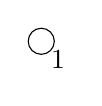
\begin{tikzpicture}[baseline=-.1cm]
  \draw(0,0) node[circle,minimum size=.2cm,draw] (A) {};
  \node [below right] at (A) {1};
\end{tikzpicture}}
+
\fgbox{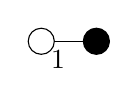
\begin{tikzpicture}[baseline=-.1cm]%{([yshift=-.3em]current bounding
% box.center)}]
  \draw(0,0) node[circle,minimum size=.2cm,draw] (A) {};
  \draw(.7,0) node[circle,minimum size=.2cm,draw,fill=black] (B) {};
  \draw (A.east) --  (B.center);
  \node [below right] at (A) {1};
\end{tikzpicture}}
+
\gbox{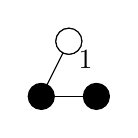
\begin{tikzpicture}[baseline=.25cm]
  \draw(0,0) node[circle,minimum size=.2cm,draw,fill=black] (A) {};
  \draw(.7,0) node[circle,minimum size=.2cm,draw,fill=black] (B) {};
  \draw(.35,.7) node[circle,minimum size=.2cm,draw] (C) {};
  \draw (A.center) --  (B.west);
  \draw (A.center) --  (C.center);
  \draw node[circle,minimum size=.2cm,draw,fill=white,opacity=1] at (C) {};
  \node [below right] at (C) {1};
\end{tikzpicture}}
+\frac 1 2
\gbox{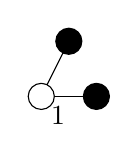
\begin{tikzpicture}[baseline=.25cm]
  \draw(.7,0) node[circle,minimum size=.2cm,draw,fill=black] (B) {};
  \draw(.35,.7) node[circle,minimum size=.2cm,draw,fill=black] (C) {};
  \draw (0,0) --  (B.center);
  \draw (0,0) --  (C.center);
  \draw(0,0) node[circle,minimum size=.2cm,draw,fill=white] (A) {};
  \node [below right] at (A) {1};
\end{tikzpicture}}
\\+& 
\frac 1 2
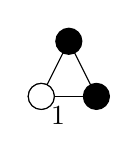
\begin{tikzpicture}[baseline=.25cm]
  \draw(0,0) node[circle,minimum size=.2cm,draw] (A) {};
  \draw(.7,0) node[circle,minimum size=.2cm,draw,fill=black] (B) {};
  \draw(.35,.7) node[circle,minimum size=.2cm,draw,fill=black] (C) {};
  \draw (A.center) --  (B.center);
  \draw (A.center) --  (C.center);
  \draw (B.center) --  (C.center);
  \draw node[circle,minimum size=.2cm,draw,fill=white,opacity=1] at (A) {};
  \node [below right] at (A) {1};
\end{tikzpicture}
 +
 \frac 1 2 
 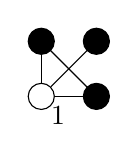
\begin{tikzpicture}[baseline=.25cm]
  \draw(0,0) node[circle,minimum size=.2cm,draw] (A) {};
  \draw(.7,0) node[circle,minimum size=.2cm,draw,fill=black] (B) {};
  \draw(0,.7) node[circle,minimum size=.2cm,draw,fill=black] (C) {};
  \draw(.7,.7) node[circle,minimum size=.2cm,draw,fill=black] (D) {};
  \draw (A.east) --  (B.center);
  \draw (A.north) --  (C.center);
  \draw (B.center) --  (C.center);
  \draw (A.north east) --  (D.center);
  \node [below right] at (A) {1};
\end{tikzpicture}
+\ldots 
\\
=&\lt\{\te{Sum of all graphs obtained from \eqref{Grand:log} by} \rt. \\
&\ph{\{}\te{turning one of the field points into a labelled}\\
&\ph{\{}\te{point.}\}
\end{aligned}
\label{Grand:reducedrho}
\end{equation}
The equations \eqref{Grand:log} and \eqref{Grand:reducedrho} are the two first major results of the MCE.
Their further simplification is one of the general goals of graph theory.
% CHECk: maybe sources necessary. Eve true?
Wertheim's approach \cite{Wertheim1} also starts developing its main advantages at this point.
However, we will not directly proceed with Wertheim's
reasoning but rather introduce a more ``classical'' way to reduce equation \eqref{Grand:reducedrho}, the
Mayer formalism. Wertheim's equations closely resemble those obtained by the Mayer formalism, and we can later
explain them by mostly analogous arguments.

\subsection{The Mayer Formalism and Topological Reduction}
\label{TopRed}
A defect of the theory we established so far is the great importance of the fugacity $z$. This quantity
is more difficult to measure than other quantities that are also easier to comprehend by intuition --
as for example the number density $\rho$.
%% CHECK: proof? http://nvlpubs.nist.gov/nistpubs/jres/090/jresv90n2p127_A1b.pdf
%%        PAPER on measurement of fugacity, But nothing specific and not up to date.
Our goal in this subsection is to determine equations for
$\ln \Xi$ and the \ep{Helmholtz free energy} $A$ that do not depend on $z$ but on $\rho$. This
would be straightforward if we could replace all occurences of $z$ by $\rho$, so it seems
a good idea to investigate the connection between those two. We already have equation
\eqref{Grand:rho}, which can be put as
\begin{equation}
\frac {\rho(1)} {z(1)} = \deri{\ln\Xi}{z(1)}.
\end{equation} 
We will see that reducing the right hand side of this equation leads to the desired
relation. Similar to \eqref{Grand:reducedrho}, we get
\begin{equation}
\begin{aligned}
\delti{\ln\Xi}{z(1)}  =
1
&+
\fgbox{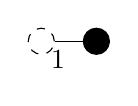
\begin{tikzpicture}[baseline=-.1cm]%{([yshift=-.3em]current bounding
% box.center)}]
  \draw(0,0) node[circle,minimum size=.2cm,dashed,draw] (A) {};
  \draw(.7,0) node[circle,minimum size=.2cm,draw,fill=black] (B) {};
  \draw (A.east) --  (B.center);
  \node [below right] at (A) {1};
\end{tikzpicture}}
+\fgbox{
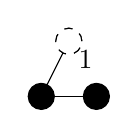
\begin{tikzpicture}[baseline=.25cm]
  \draw(0,0) node[circle,minimum size=.2cm,draw,fill=black] (A) {};
  \draw(.7,0) node[circle,minimum size=.2cm,draw,fill=black] (B) {};
  \draw(.35,.7) node[circle,minimum size=.2cm,dashed,draw] (C) {};
  \draw (A.center) --  (B.west);
  \draw (A.center) --  (C.center);
  \draw node[circle,minimum size=.2cm,draw,fill=white,dashed,opacity=1] at (C) {};
  \node [below right] at (C) {1};
\end{tikzpicture}}
+\frac 1 2
\begin{tikzpicture}[baseline=.25cm]
  \draw(.7,0) node[circle,minimum size=.2cm,draw,fill=black] (B) {};
  \draw(.35,.7) node[circle,minimum size=.2cm,draw,fill=black] (C) {};
  \draw (0,0) --  (B.center);
  \draw (0,0) --  (C.center);
  \draw(0,0) node[circle,minimum size=.2cm,draw,dashed,fill=white] (A) {};
  \node [below right] at (A) {1};
\end{tikzpicture}
\\&+ 
\frac 1 2
\begin{tikzpicture}[baseline=.25cm]
  \draw(0,0) node[circle,minimum size=.2cm,dashed,draw] (A) {};
  \draw(.7,0) node[circle,minimum size=.2cm,draw,fill=black] (B) {};
  \draw(.35,.7) node[circle,minimum size=.2cm,draw,fill=black] (C) {};
  \draw (A.center) --  (B.center);
  \draw (A.center) --  (C.center);
  \draw (B.center) --  (C.center);
  \draw node[circle,minimum size=.2cm,draw,dashed,fill=white,opacity=1] at (A) {};
  \node [below right] at (A) {1};
\end{tikzpicture}
 +
 \frac 1 2 
 \begin{tikzpicture}[baseline=.25cm]
  \draw(0,0) node[circle,minimum size=.2cm,dashed,draw] (A) {};
  \draw(.7,0) node[circle,minimum size=.2cm,draw,fill=black] (B) {};
  \draw(0,.7) node[circle,minimum size=.2cm,draw,fill=black] (C) {};
  \draw(.7,.7) node[circle,minimum size=.2cm,draw,fill=black] (D) {};
  \draw (A.east) --  (B.center);
  \draw (A.north) --  (C.center);
  \draw (B.center) --  (C.center);
  \draw (A.north east) --  (D.center);
  \node [below right] at (A) {1};
\end{tikzpicture}
+\ldots 
\end{aligned}
\end{equation}
This sum falls under the prerequisites of Lemma \ref{lemma:articulation}: all graphs contained
can be uniquely expressed as products of graphs where the labelled point $1$ is not an articulation point, 
and if one joins any graphs where $1$ is not an articulation point together, the result is 
exactly one graph in the sum. We can use \eqref{Lemma6:eq} and define a new function $c(1)$,
which is sometimes referred to as the \ep{correlation function} (also called $h(1)$ by
some authors \cite{Stell}). It is given by
\begin{equation}
c(1):=\ln\lt[\frac {\rho(1)} {z(1)}\rt],
\label{TopRed:cDefi}
\end{equation}
and using the above simplifications, it is
\begin{equation}
\begin{aligned}
c(1)=&
\fgbox{\begin{tikzpicture}[baseline=-.1cm]%{([yshift=-.3em]current bounding
% box.center)}]
  \draw(0,0) node[circle,minimum size=.2cm,dashed,draw] (A) {};
  \draw(.7,0) node[circle,minimum size=.2cm,draw,fill=black] (B) {};
  \draw (A.east) --  (B.center);
  \node [below right] at (A) {1};
\end{tikzpicture}}
+
\gbox{\begin{tikzpicture}[baseline=.25cm]
  \draw(0,0) node[circle,minimum size=.2cm,draw,fill=black] (A) {};
  \draw(.7,0) node[circle,minimum size=.2cm,draw,fill=black] (B) {};
  \draw(.35,.7) node[circle,minimum size=.2cm,dashed,draw] (C) {};
  \draw (A.center) --  (B.west);
  \draw (A.center) --  (C.center);
  \draw node[circle,minimum size=.2cm,draw,fill=white,dashed,opacity=1] at (C) {};
  \node [below right] at (C) {1};
\end{tikzpicture}}
+ 
\frac 1 2
\begin{tikzpicture}[baseline=.25cm]
  \draw(0,0) node[circle,minimum size=.2cm,dashed,draw] (A) {};
  \draw(.7,0) node[circle,minimum size=.2cm,draw,fill=black] (B) {};
  \draw(.35,.7) node[circle,minimum size=.2cm,draw,fill=black] (C) {};
  \draw (A.center) --  (B.center);
  \draw (A.center) --  (C.center);
  \draw (B.center) --  (C.center);
  \draw node[circle,minimum size=.2cm,draw,dashed,fill=white,opacity=1] at (A) {};
  \node [below right] at (A) {1};
\end{tikzpicture}
 + 
 \begin{tikzpicture}[baseline=.25cm]
  \draw(0,0) node[circle,minimum size=.2cm,dashed,draw] (A) {};
  \draw(.7,0) node[circle,minimum size=.2cm,draw,fill=black] (B) {};
  \draw(0,.7) node[circle,minimum size=.2cm,draw,fill=black] (C) {};
  \draw(.7,.7) node[circle,minimum size=.2cm,draw,fill=black] (D) {};
  \draw (A.east) --  (B.center);
  \draw (A.north) --  (C.center);
  \draw (B.center) --  (C.center);
  \draw (C.center) --  (D.center);
  \node [below right] at (A) {1};
\end{tikzpicture}
\\
+&
\frac 1 2
 \begin{tikzpicture}[baseline=.25cm]
  \draw(0,0) node[circle,minimum size=.2cm,dashed,draw] (A) {};
  \draw(.7,0) node[circle,minimum size=.2cm,draw,fill=black] (B) {};
  \draw(0,.7) node[circle,minimum size=.2cm,draw,fill=black] (C) {};
  \draw(.7,.7) node[circle,minimum size=.2cm,draw,fill=black] (D) {};
  \draw (A.north) --  (C.center);
  \draw (B.center) --  (C.center);
  \draw (C.center) --  (D.center);
  \node [below right] at (A) {1};
\end{tikzpicture}
+
 \begin{tikzpicture}[baseline=.25cm]
  \draw(0,0) node[circle,minimum size=.2cm,dashed,draw] (A) {};
  \draw(.7,0) node[circle,minimum size=.2cm,draw,fill=black] (B) {};
  \draw(0,.7) node[circle,minimum size=.2cm,draw,fill=black] (C) {};
  \draw(.7,.7) node[circle,minimum size=.2cm,draw,fill=black] (D) {};
  \draw (A.north) --  (C.center);
  \draw (B.center) --  (D.center);
  \draw (C.center) --  (D.center);
  \node [below right] at (A) {1};
\end{tikzpicture}
+
\ldots 
\\
=&\{\te{Sum of all graphs with one labelled point 1}\\
&\ph{\{}\te {and }N_z\ge 1\ z\te{ field points connected by } f \te{-bonds}\\
&\ph{\{}\te{such that the labelled point is no articulation}\\
&\ph{\{}\te{point.}\}
%\\
%&=\{\mbox{\parbox{Let's try to have fun with a lot of text in this mbox which does not break shit}}\}
\end{aligned}
\label{TopRed:c(1)}
\end{equation}
Equation \eqref{TopRed:c(1)} contains all of the graphs with $N\le3$ points in $c(1)$ and some
of those with  $N=4$ points. We chose them to illustrate the next step in our reduction. We already
used the fact that in some graphs of $\rho$ the labelled point is an articulation point. However,
there are also numerous graphs where at least one field point is an articulation point. These are
still contained in $c(1)$, in \eqref{TopRed:c(1)} they are in the second, forth, fifth and sixth
graph.
%% CHECK: terrible explanation
These graphs can all be constructed from an at least doubly connected
subgraph containing the labelled point and a graph from $\rho$ in
\eqref{Grand:reducedrho} attached to each field point such that the field point
is overwritten by the labelled point in $\rho$. The attached graph may be the
one point graph. One can group all the graphs in $c(1)$ into equivalence
classes by defining the \ep{maximal connected subgraph} $\Ga_m$ for any graph
$\Ga$: it is the subgraph with the most field points in the set of subgraphs
free of articulation field points that contain the labelled point. Since the
labelled point is not an articulation point in the graphs of $c(1)$, $\Ga_m$ is
unique for any $\Ga$ in $c(1)$. If we now look at all the graphs contained in
one of the equivalence classes defined by $\Ga_m$, we see that it contains
exactly all graphs obtainable by attaching graphs from $\rho$ to the field
points in the manner described above. We can therefore use the idea of changing
the property of a point we described in Section \ref{ArtPoint} and change the
property of the field points from $z(1)$ to $\rho(1)$. Then, we can express $c(1)$ by
\begin{equation}
\begin{aligned}
c(1)=& \fgbox{ 
\begin{tikzpicture}[baseline=-.1cm]%{([yshift=-.3em]current bounding box.center)}]
  \draw(0,0) node[circle,minimum size=.2cm,dashed,draw] (A) {};
  \draw(.7,0) node[circle,minimum size=.2cm,draw,fill=blue, opacity=1] (B) {};
  \draw (A.east) --  (B.west);
  \node [below right] at (A) {1};
\end{tikzpicture}}
+
\frac 1 2
\begin{tikzpicture}[baseline=.25cm]
  \draw(0,0) node[circle,minimum size=.2cm,dashed,draw,fill=white] (A) {};
  \draw(.7,0) node[circle,minimum size=.2cm,draw,fill=blue] (B) {};
  \draw(.35,.7) node[circle,minimum size=.2cm,draw,fill=blue] (C) {};
\begin{pgfonlayer}{background}
  \draw (A.center) --  (B.center);
  \draw (A.center) --  (C.center);
  \draw (B.center) --  (C.center);
\end{pgfonlayer}
%  \draw node[circle,minimum size=.2cm,draw,dashed,fill=white,opacity=1] at (A) {};
  \node [below right] at (A) {1};
\end{tikzpicture}
 + 
\frac 1 2
 \begin{tikzpicture}[baseline=.25cm]
  \draw(0,0) node[circle,minimum size=.2cm,dashed,fill=white,draw] (A) {};
  \draw(.7,0) node[circle,minimum size=.2cm,draw,fill=blue] (B) {};
  \draw(.7,.7) node[circle,minimum size=.2cm,draw,fill=blue] (C) {};
  \draw(0,.7) node[circle,minimum size=.2cm,draw,fill=blue] (D) {};
\begin{pgfonlayer}{background}
  \draw (A.center) --  (B.center);
  \draw (B.center) --  (C.center);
  \draw (C.center) --  (D.center);
  \draw (D.center) --  (A.center);
  \draw (B.center) --  (D.center);
\end{pgfonlayer}
  \node [below right] at (A) {1};
\end{tikzpicture}
+
\frac 1 2
 \begin{tikzpicture}[baseline=.25cm]
  \draw(0,0) node[circle,minimum size=.2cm,dashed,fill=white,draw] (A) {};
  \draw(.7,0) node[circle,minimum size=.2cm,draw,fill=blue] (B) {};
  \draw(.7,.7) node[circle,minimum size=.2cm,draw,fill=blue] (C) {};
  \draw(0,.7) node[circle,minimum size=.2cm,draw,fill=blue] (D) {};
\begin{pgfonlayer}{background}
  \draw (A.center) --  (B.center);
  \draw (B.center) --  (C.center);
  \draw (C.center) --  (D.center);
  \draw (D.center) --  (A.center);
  \draw (A.center) --  (C.center);
\end{pgfonlayer}
  \node [below right] at (A) {1};
\end{tikzpicture}
\\
+&
\frac 1 2
 \begin{tikzpicture}[baseline=.25cm]
  \draw(0,0) node[circle,minimum size=.2cm,dashed,fill=white,draw] (A) {};
  \draw(.7,0) node[circle,minimum size=.2cm,draw,fill=blue] (B) {};
  \draw(.7,.7) node[circle,minimum size=.2cm,draw,fill=blue] (C) {};
  \draw(0,.7) node[circle,minimum size=.2cm,draw,fill=blue] (D) {};
\begin{pgfonlayer}{background}
  \draw (A.center) --  (B.center);
  \draw (B.center) --  (C.center);
  \draw (C.center) --  (D.center);
  \draw (D.center) --  (A.center);
\end{pgfonlayer}
  \node [below right] at (A) {1};
\end{tikzpicture}
+
\frac 1 6
 \begin{tikzpicture}[baseline=.25cm]
  \draw(0,0) node[circle,minimum size=.2cm,dashed,fill=white,draw] (A) {};
  \draw(.7,0) node[circle,minimum size=.2cm,draw,fill=blue] (B) {};
  \draw(.7,.7) node[circle,minimum size=.2cm,draw,fill=blue] (C) {};
  \draw(0,.7) node[circle,minimum size=.2cm,draw,fill=blue] (D) {};
\begin{pgfonlayer}{background}
  \draw (A.center) --  (B.center);
  \draw (B.center) --  (C.center);
  \draw (C.center) --  (D.center);
  \draw (D.center) --  (A.center);
  \draw (A.center) --  (C.center);
  \draw (B.center) --  (D.center);
\end{pgfonlayer}
  \node [below right] at (A) {1};
\end{tikzpicture}
+
\ldots 
\\
=&\{\te{Sum of all graphs with one labelled point 1,}\\
&\ N_\rho\ge 1\ \rho\te{ field points connected by } f \te{-bonds}\\
&\ \te{such that none of the points is an articulation}\\
&\ \te{point.}\}
%\\
%&=\{\mbox{\parbox{Let's try to have fun with a lot of text in this mbox which does not break shit}}\}
\end{aligned}
\label{TopRed:c(1)ByRho}
\end{equation}       
This equation contains all of the graphs with $N\le4$ points in $c(1)$. We use blue points to mark $\rho$ field points. Using the definition
of $c(1)$ and the fact that we can express $c(1)$ purely $\rho$ dependent, we can now express $z(1)$ with respect to $\rho$ by
inserting \eqref{TopRed:c(1)ByRho} into \eqref{TopRed:cDefi}, which yields
\begin{equation}
\ln z(1) = \ln \rho(1) - c(1).
\label{TopRed:zbyRho}
\end{equation}
With these equations, we are able to give a $\rho$ dependent version of $\ln \Xi$. We start with
the variation given by \eqref{FuncDeri}, which is for $\ln \Xi$
\begin{equation}
\begin{aligned}
\dl \ln\Xi &= \int \di(1) \delti{\ln\Xi} {z(1)}\ \dl z(1) \\
&= \int \di(1) \rho(1) \frac{\dl z(1)}{z(1)} \\
&= \int \di(1) \rho(1)\ \dl \lt[\ln z(1)\rt]  \\
&= \int \di(1) \rho(1)\ \dl\lt[ \ln \rho(1) - c(1) \rt] \\
&= \int \di(1) \lt[\dl \rho(1)\ - \dl \lt[\rho(1)c(1)\rt] + c(1)\ \dl\rho(1) \rt].
\end{aligned}
\label{TopRed:deltalnXi halfway}
\end{equation}  
If there were a function $\cze$ with the property
\begin{equation}
c(1) = \delti \cze {\rho(1)},
\label{TopRed:czebyderi} 
\end{equation}
then \eqref{TopRed:deltalnXi halfway} could be written
\begin{equation}
\dl \ln \Xi = \dl \lt[\int\di(1) \rho(1) - \int\di(1) \rho(1)c(1) + \cze\rt].
\label{TopRed:deltalnXi finished} 
\end{equation}
This implies
\begin{equation}
\ln \Xi = \int\di(1) \rho(1) - \int\di(1) \rho(1)c(1) + \cze,
\label{TopRed:lnxi final} 
\end{equation}
where we ignored the possible addition of a constant, as it is unimportant in a thermodynamic
potential. The only chore left is to find the missing graph sum \cze. It is however easy
to guess from \eqref{TopRed:c(1)ByRho}. It must be
\begin{equation}
\begin{aligned}
\cze=&
\frac 1 2
\begin{tikzpicture}[baseline=-.1cm]%{([yshift=-.3em]current bounding box.center)}]
  \draw(0,0) node[circle,minimum size=.2cm,fill=blue,draw] (A) {};
  \draw(.7,0) node[circle,minimum size=.2cm,draw,fill=blue, opacity=1] (B) {};
  \draw (A.east) --  (B.west);
\end{tikzpicture}
+
\ph{.}\frac 1 6\ph{.}
\begin{tikzpicture}[baseline=.25cm]
  \draw(0,0) node[circle,minimum size=.2cm,fill=blue,draw] (A) {};
  \draw(.7,0) node[circle,minimum size=.2cm,draw,fill=blue] (B) {};
  \draw(.35,.7) node[circle,minimum size=.2cm,draw,fill=blue] (C) {};
\begin{pgfonlayer}{background}
  \draw (A.center) --  (B.center);
  \draw (A.center) --  (C.center);
  \draw (B.center) --  (C.center);
\end{pgfonlayer}
\end{tikzpicture}
 + 
\frac 1 4
 \begin{tikzpicture}[baseline=.25cm]
  \draw(0,0) node[circle,minimum size=.2cm,fill=blue,draw] (A) {};
  \draw(.7,0) node[circle,minimum size=.2cm,draw,fill=blue] (B) {};
  \draw(.7,.7) node[circle,minimum size=.2cm,draw,fill=blue] (C) {};
  \draw(0,.7) node[circle,minimum size=.2cm,draw,fill=blue] (D) {};
\begin{pgfonlayer}{background}
  \draw (A.center) --  (B.center);
  \draw (B.center) --  (C.center);
  \draw (C.center) --  (D.center);
  \draw (D.center) --  (A.center);
  \draw (B.center) --  (D.center);
\end{pgfonlayer}
\end{tikzpicture}
\\+&
\frac 1 8
 \begin{tikzpicture}[baseline=.25cm]
  \draw(0,0) node[circle,minimum size=.2cm,fill=blue,draw] (A) {};
  \draw(.7,0) node[circle,minimum size=.2cm,draw,fill=blue] (B) {};
  \draw(.7,.7) node[circle,minimum size=.2cm,draw,fill=blue] (C) {};
  \draw(0,.7) node[circle,minimum size=.2cm,draw,fill=blue] (D) {};
\begin{pgfonlayer}{background}
  \draw (A.center) --  (B.center);
  \draw (B.center) --  (C.center);
  \draw (C.center) --  (D.center);
  \draw (D.center) --  (A.center);
\end{pgfonlayer}
\end{tikzpicture}
+
\frac 1 {24}
 \begin{tikzpicture}[baseline=.25cm]
  \draw(0,0) node[circle,minimum size=.2cm,fill=blue,draw] (A) {};
  \draw(.7,0) node[circle,minimum size=.2cm,draw,fill=blue] (B) {};
  \draw(.7,.7) node[circle,minimum size=.2cm,draw,fill=blue] (C) {};
  \draw(0,.7) node[circle,minimum size=.2cm,draw,fill=blue] (D) {};
\begin{pgfonlayer}{background}
  \draw (A.center) --  (B.center);
  \draw (B.center) --  (C.center);
  \draw (C.center) --  (D.center);
  \draw (D.center) --  (A.center);
  \draw (A.center) --  (C.center);
  \draw (B.center) --  (D.center);
\end{pgfonlayer}
\end{tikzpicture}
+
\ldots 
\\
=&\{\te{Sum of all connected graphs with } N \ge 2\ \\
&\ph{\{}\rho \te{ field points connected by } f \te{-bonds such }\\
&\ph{\{}\te{that none of the points is an articulation point.}\}
%\\
%&=\{\mbox{\parbox{Let's try to have fun with a lot of text in this mbox which does not break shit}}\}
\end{aligned}
\label{TopRed:czeGraph}
\end{equation}
Since the symmetry numbers are changed adequately by the process of derivation, \cze
given by \eqref{TopRed:czeGraph} satisfies \eqref{TopRed:czebyderi}.

From an expression for $\ln\Xi$, which gives us an equation of state by the relation
\eqref{bpV}, we can also derive an expression for the free energy $A$. It is related to
the grand canonical potential $\Om$ by
\begin{equation}
\be A = \be \Om + \be\mu \bar N = - \ln \Xi + \ln \lt(z \lath^3\rt) \bar N.
\label{TopRed:beA_1} 
\end{equation}
We can do some rearrangments by remembering that $z(1)\equiv z$ is constant and using
equation \eqref{Nbyrho}, \eqref{TopRed:zbyRho} and \eqref{TopRed:deltalnXi finished},
which leads to
\begin{equation}
\begin{aligned}
\be A &= - \int\di(1) \rho(1) + \int\di(1) \rho(1)c(1) - \cze \\
&\qquad + \int \di(1) \rho(1) \ln \lt(z(1) \lath^3\rt)  \\
&= \int \di(1) \rho(1) \lt [ \ln\lt(\rho(1)\lath^3\rt) - 1\rt] - \cze.
\end{aligned}
\label{TopRed:beA_2} 
\end{equation}
We have therefore reached the goal of this section and derived equations for $\ln \Xi$ and $\be A$
that do not depend on the possibly disadvantageous property $z$ but on the number density $\rho$.
Before proceeding, we want to introduce a different class of functions that are often
of interest to thermodynamic models. One may consider them a generalization of
$c(1)$ to multiple labelled points and they, too, are called correlation
functions.

%\newcommand\rs{\rho^{(s)}}
\newcommand\os{1,\ldots,s}
\newcommand\ros{\rho(1\cdots s)}
\newcommand\uos{u(1\cdots s)}
% \newcommand\ros{\rho^{(s)}(1\cdots s)}
% \newcommand\uos{u^{(s)}(1\cdots s)}
\subsection{$s$-Particle Distribution and Correlation Functions}
\label{MCE:sPart} 
The function $\rho(1)$ describes the particle density at location 1 (possibly including
orientation). Obviously, there may be functions $\ros$ that describe the density of
$s$ particles -- or, in that case more accurately, their distribution -- at the
locations $\os$. They are described by a more general form of \eqref{Grand:rho},
\begin{equation}
\begin{aligned}
\ros%=& \lara{\dl(\cd-1)\cdots\dl(\cd-s)}_\Xi\\
=&\sum_{N=s}^{\infty} \int\di(s)\cdots\di(N) \frac{N!}{(N-s)!}P(N;\r^N),
\end{aligned}
\label{sPart:ros.simple}
\end{equation}
which again is the result for calculating the canonical average of delta peaks. We can simplify
\eqref{sPart:ros.simple} to
\begin{equation}
\ros=\frac 1 \Xi \prod_{i=1}^s z(i) \frac{\dl^s\Xi}{\prod_{i=1}^s \dl z(i)}.
\label{sPart:ros.byXi}
\end{equation} 
This time, we can not jump straight to the logarithm for which we have a representation by connected
graphs. However, we can define the \ep{Ursell functions} 
%% CHECK: Definition necessary?
\begin{equation}
\uos:=\prod_{i=1}^s z(i) \frac{\dl^s \ln \Xi}{\prod_{i=1}^s \dl z(i)}
\end{equation}
that are in close relation to $\ros$. To investigate this relation, we
define for $s \ge 2$ the \ep{correlation functions}
\newcommand\g{g(12)}
\renewcommand\h{h(12)}
\begin{equation}
h(1\cdots s)=\frac{\uos}{\rho(1)\cdots\rho(s)}
\label{sPart:hsimple}
\end{equation}
and
\begin{equation}
g(1\cdots s)=\frac{\ros}{\rho(1)\cdots\rho(s)}.
\label{sPart:gsimple}
\end{equation}
In the special case of $s=1$, we already met the function $h(1)$, which is the
same as $c(1)$ in \eqref{TopRed:cDefi}. We can now consider the relationship
between the $\uos$ functions and the $\ros$ functions, starting with the obvious
case of
\begin{equation}
u(1)=\rho(1).
%u^{(1)}(1)=\rho(1).
\end{equation}
For $s=2$, we find
% \newcommand\ut{u^{(2)}(12)}
% \newcommand\rot{\rho^{(2)}(12)}
\newcommand\ut{u(12)}
\newcommand\rot{\rho(12)}
\begin{equation}
\begin{aligned}
\ut=&z(1)z(2)\frac\dl{z(2)} \frac 1 \Xi \deri{\Xi}{z(1)}\\
=&z(1)z(2)\ed{\frac 1 \Xi \frac{\dl^2 \Xi}{\dl z(1) \dl z(2)} - \frac 1 {\Xi^2} \deri{\Xi}{z(1)} \deri{\Xi}{z(2)}}\\
=&\rot - \rho(1)\rho(2).
\end{aligned}
\label{sPart:UByRho}
\end{equation}
It becomes evident that by an analogous procedure any $\ros$ can be described by $u(1\cdots r)$ with $r\le s$.
Since the $\uos$ are all sums of graphs obtained from $\ln \Xi$ by turning $s$ field points into labelled points,
$\ros$ will have a similar form.
% Even better, it is possible to express an $s$-particle distribution
%entirely by $1$-particle distribution functions times $g(\os)$ or $h(\os)$ by
%\eqref{sPart:gsimple} and \eqref{sPart:hsimple}.
We will explain this with the example of the two-particle correlation functions
$\g$ and $\h$. Let us look closer at $\ut$. It contains

\newcommand\twoart{
  \draw(0,0) node[circle,minimum size=.2cm,draw] (A) {};
  \draw(.7,0) node[circle,minimum size=.2cm,draw] (B) {};
  \node at (.23,-.17) {\footnotesize 1};
  \node at (.93,-.17) {\footnotesize 2};
}
\newcommand\threeart{
\begin{pgfonlayer}{main}
  \draw(0,0) node[circle,minimum size=.2cm,fill=white,draw] (A) {};
  \draw(.7,0) node[circle,minimum size=.2cm,fill=white,draw] (B) {};
  \draw(.35,.7) node[circle,minimum size=.2cm,fill=black,draw] (C) {};
  \node at (.23,-.17) {\footnotesize 1};
  \node at (.93,-.17) {\footnotesize 2};
\end{pgfonlayer}
}
\newcommand\fourart{
\begin{pgfonlayer}{main}
  \draw(0,0) node[circle,minimum size=.2cm,fill=white,draw] (A) {};
  \draw(.7,0) node[circle,minimum size=.2cm,draw,fill=white] (B) {};
  \draw(.7,.7) node[circle,minimum size=.2cm,draw,fill=black] (C) {};
  \draw(0,.7) node[circle,minimum size=.2cm,draw,fill=black] (D) {};
  \node at (.23,-.17) {\footnotesize 1};
  \node at (.93,-.17) {\footnotesize 2};
\end{pgfonlayer}
}

\begin{equation}
\begin{aligned}
\ut=&
\begin{tikzpicture}[baseline=-.1cm]%{([yshift=-.3em]current bounding box.center)}]
  \twoart
  \draw (A.east) --  (B.west);
\end{tikzpicture}
+
\begin{tikzpicture}[baseline=.25cm]
\threeart
\begin{pgfonlayer}{background}
  \draw (A.center) --  (B.center);
  \draw (A.center) --  (C.center);
\end{pgfonlayer}
\end{tikzpicture}
+
 \begin{tikzpicture}[baseline=.25cm]
\threeart
\begin{pgfonlayer}{background}
  \draw (A.center) --  (B.center);
  \draw (B.center) --  (C.center);
\end{pgfonlayer}
\end{tikzpicture}
+
\begin{tikzpicture}[baseline=.25cm]
\threeart
\begin{pgfonlayer}{background}
  \draw (A.center) --  (C.center);
  \draw (B.center) --  (C.center);
\end{pgfonlayer}
\end{tikzpicture} 
\\
+&
\begin{tikzpicture}[baseline=.25cm]
\threeart
\begin{pgfonlayer}{background}
  \draw (A.center) --  (B.center);
  \draw (A.center) --  (C.center);
  \draw (B.center) --  (C.center);
\end{pgfonlayer}
\end{tikzpicture}
 +
 \begin{tikzpicture}[baseline=.25cm]
  \fourart
\begin{pgfonlayer}{background}
  \draw (A.center) --  (B.center);
  \draw (B.center) --  (C.center);
  \draw (A.center) --  (D.center);
\end{pgfonlayer}
 \end{tikzpicture}
+
 \begin{tikzpicture}[baseline=.25cm]
  \fourart
\begin{pgfonlayer}{background}
  \draw (A.center) --  (B.center);
  \draw (B.center) --  (C.center);
  \draw (A.center) --  (D.center);
  \draw (A.center) --  (C.center);
\end{pgfonlayer}
 \end{tikzpicture}
 +
 \begin{tikzpicture}[baseline=.25cm]
  \fourart
\begin{pgfonlayer}{background}
  \draw (A.center) --  (B.center);
  \draw (B.center) --  (C.center);
  \draw (A.center) --  (D.center);
  \draw (B.center) --  (D.center);
\end{pgfonlayer}
 \end{tikzpicture}\\
+&
 \begin{tikzpicture}[baseline=.25cm]
  \fourart
\begin{pgfonlayer}{background}
  \draw (A.center) --  (B.center);
  \draw (B.center) --  (C.center);
  \draw (C.center) --  (D.center);
  \draw (D.center) --  (A.center);
\end{pgfonlayer}
\end{tikzpicture}
+
\begin{tikzpicture}[baseline=.25cm]
  \fourart
\begin{pgfonlayer}{background}
  \draw (B.center) --  (C.center);
  \draw (C.center) --  (D.center);
  \draw (D.center) --  (A.center);
\end{pgfonlayer}
\end{tikzpicture}
+ \ldots
%  \frac 1 2
%  \begin{tikzpicture}[baseline=.25cm]
%   \fourart
% \begin{pgfonlayer}{background}
%   \draw (A.center) --  (B.center);
%   \draw (B.center) --  (C.center);
%   \draw (C.center) --  (D.center);
%   \draw (D.center) --  (A.center);
%   \draw (A.center) --  (C.center);
%   \draw (B.center) --  (D.center);
% \end{pgfonlayer}
% \end{tikzpicture}
% +
% \frac 1 2
%  \begin{tikzpicture}[baseline=.25cm]
%   \fourart
% \begin{pgfonlayer}{background}
%   \draw (B.center) --  (C.center);
%   \draw (C.center) --  (D.center);
%   \draw (D.center) --  (A.center);
%   \draw (A.center) --  (C.center);
%   \draw (B.center) --  (D.center);
% \end{pgfonlayer}
% \end{tikzpicture}
\end{aligned}
\end{equation} 
We can see that any graph in $\ut$ can be constructed from a subgraph in which
none of the labelled points is an articulation point (the field points may
still be articulation points) and a graph from $\rho(1)$ appended
(i.e. multiplied) to the point 1 and a graph from $\rho(2)$ to the point 2.
Note that the subgraph is thus unique. The sum over all these subgraphs is the correlation function $\h$, given by
\renewcommand\twoart{
  \draw(0,0) node[circle,minimum size=.2cm,dashed,fill=white,draw] (A) {};
  \draw(.7,0) node[circle,minimum size=.2cm,dashed,fill=white,draw] (B) {};
  \node at (.23,-.17) {\footnotesize 1};
  \node at (.93,-.17) {\footnotesize 2};
}
\renewcommand\threeart{
\begin{pgfonlayer}{main}
  \twoart
  \draw(.35,.7) node[circle,minimum size=.2cm,fill=black,draw] (C) {};
\end{pgfonlayer}
}
\renewcommand\fourart{
\begin{pgfonlayer}{main}
  \twoart
  \draw(.7,.7) node[circle,minimum size=.2cm,draw,fill=black] (C) {};
  \draw(0,.7) node[circle,minimum size=.2cm,draw,fill=black] (D) {};
\end{pgfonlayer}
}
\begin{equation}
\begin{aligned}
\h=&
\begin{tikzpicture}[baseline=-.1cm]%{([yshift=-.3em]current bounding box.center)}]
  \twoart
  \draw (A.east) --  (B.west);
\end{tikzpicture}
+
\begin{tikzpicture}[baseline=.25cm]
\threeart
\begin{pgfonlayer}{background}
  \draw (A.center) --  (C.center);
  \draw (B.center) --  (C.center);
\end{pgfonlayer}
\end{tikzpicture} 
+
\begin{tikzpicture}[baseline=.25cm]
\threeart
\begin{pgfonlayer}{background}
  \draw (A.center) --  (B.center);
  \draw (A.center) --  (C.center);
  \draw (B.center) --  (C.center);
\end{pgfonlayer}
\end{tikzpicture}\\
 +&
 \begin{tikzpicture}[baseline=.25cm]
  \fourart
\begin{pgfonlayer}{background}
  \draw (A.center) --  (B.center);
  \draw (B.center) --  (C.center);
  \draw (C.center) --  (D.center);
  \draw (D.center) --  (A.center);
\end{pgfonlayer}
\end{tikzpicture}
+
\begin{tikzpicture}[baseline=.25cm]
  \fourart
\begin{pgfonlayer}{background}
  \draw (B.center) --  (C.center);
  \draw (C.center) --  (D.center);
  \draw (D.center) --  (A.center);
\end{pgfonlayer}
\end{tikzpicture}
+ \ldots\\
=&\{\te{Sum of all connected graphs consisting of} \\
&\phantom{\{}\te{labelled points } 1 \te{ and } 2 \te{, $z$-field points and} \\
&\phantom{\{}\te{$f$-bonds. No labelled point is an articulation}\\
&\phantom{\{}\te{point.}\}
\end{aligned}
\label{sPoint:h}
\end{equation}
where dashed points are again points without property. Alongside \eqref{sPart:UByRho}, this leads to
\begin{equation}
\rot=\rho(1)\h\rho(2)+\rho(1)\rho(2)=\rho(1)\g\rho(2).
\end{equation} 
Here, $g$ is simply
\begin{equation}
\g=\h+1.
\end{equation} 
1 is also the value of the graph containing two unbonded labelled points without property. If we add it
to \eqref{sPoint:h}, we see that for any graph in $\g$ where there is an $f$-bond between the labelled
points, there is also a graph in $\g$ where there is no bond between the two, and vice versa. The sum
of an $f$-bond and no bond is an $e$-bond. We can therefore write
\renewcommand\twoart{
  \draw(0,0) node[circle,minimum size=.2cm,dashed,fill=white,draw] (A) {};
  \draw(.7,0) node[circle,minimum size=.2cm,dashed,fill=white,draw] (B) {};
  \node at (.23,-.17) {\footnotesize 1};
  \node at (.93,-.17) {\footnotesize 2};
  \draw (A.east) -- (B.west) [dashed];
}
%\renewcommand\threeart{
%\begin{pgfonlayer}{main}
%  \twoart
%  \draw(.35,.7) node[circle,minimum size=.2cm,fill=black,draw] (C) {};
%\end{pgfonlayer}
%}
%\renewcommand\fourart{
%\begin{pgfonlayer}{main}
%  \twoart
%  \draw(.7,.7) node[circle,minimum size=.2cm,draw,fill=black] (C) {};
%  \draw(0,.7) node[circle,minimum size=.2cm,draw,fill=black] (D) {};
%\end{pgfonlayer}
%}
\begin{equation}
\begin{aligned}
\g=&
\begin{tikzpicture}[baseline=-.1cm]%{([yshift=-.3em]current bounding box.center)}]
  \twoart
\end{tikzpicture}
+
\begin{tikzpicture}[baseline=.25cm]
\threeart
\begin{pgfonlayer}{background}
  \draw (A.center) --  (C.center);
  \draw (B.center) --  (C.center);
\end{pgfonlayer}
\end{tikzpicture} 
+
\begin{tikzpicture}[baseline=.25cm]
  \fourart
\begin{pgfonlayer}{background}
  \draw (B.center) --  (C.center);
  \draw (C.center) --  (D.center);
  \draw (D.center) --  (A.center);
\end{pgfonlayer}
\end{tikzpicture}
+ \ldots \\
=&\{\te{Sum of all connected graphs consisting of} \\
&\phantom{\{}\te{labelled points } 1 \te{ and } 2 \te{ connected by an } \\
&\phantom{\{}e\te{-bond and a network of }z\te{ field points and}\\
&\phantom{\{}\te{$f$-bonds. No labelled point is an articulation}\\
&\phantom{\{}\te{point.}\}
\end{aligned}
\label{sPoint:g}
\end{equation}
Dashed bonds are $e$-bonds. It is possible to further reduce $\g$ by the same
arguments we used to reduce $c(1)$. Since the field points may still be
field articulation points, the sum in $\g$ contains maximal articulation point
free subgraphs and all graphs resulting from appending some graph of $\rho(1)$ to
each field point. We can therefore replace $z$ field points by $\rho$ field
points in \eqref{sPoint:g}, arriving at \renewcommand\threeart{
\begin{pgfonlayer}{main}
  \twoart
  \draw(.35,.7) node[circle,minimum size=.2cm,fill=blue,draw] (C) {};
\end{pgfonlayer}
}
\renewcommand\fourart{
\begin{pgfonlayer}{main}
  \twoart
  \draw(.7,.7) node[circle,minimum size=.2cm,draw,fill=blue] (C) {};
  \draw(0,.7) node[circle,minimum size=.2cm,draw,fill=blue] (D) {};
\end{pgfonlayer}
}
\begin{equation}
\begin{aligned}
\g=&
\begin{tikzpicture}[baseline=-.1cm]%{([yshift=-.3em]current bounding box.center)}]
  \twoart
\end{tikzpicture}
+
\begin{tikzpicture}[baseline=.25cm]
\threeart
\begin{pgfonlayer}{background}
  \draw (A.center) --  (C.center);
  \draw (B.center) --  (C.center);
\end{pgfonlayer}
\end{tikzpicture} 
+
\begin{tikzpicture}[baseline=.25cm]
  \fourart
\begin{pgfonlayer}{background}
  \draw (B.center) --  (C.center);
  \draw (C.center) --  (D.center);
  \draw (D.center) --  (A.center);
\end{pgfonlayer}
\end{tikzpicture}
+ \ldots \\
=&\{\te{Sum of all at least doubly connected graphs} \\
&\phantom{\{}\te{consisting of labelled points } 1 \te{ and  $2$ connec-} \\
&\phantom{\{}\te{ted by an }e\te{-bond and a network of $\rho$ field} \\
&\phantom{\{}\te{points and $f$-bonds.\}}
\end{aligned}
\label{sPoint:gbyrho}
\end{equation}
This concludes the remarks on correlation functions for now.

\section{Wertheim's Multiple Density Formalism}
\label{WH}
The approach presented in the previous section is rather general, since we have
not committed to any forms of the interaction potential $\phi(12)$. Of course, when
choosing a specific class of $\phi(12)$, it may be advisable to also undertake
variations to the process of graph reduction. One of these variations was
presented by M. S. Wertheim in 1983 \cite{Wertheim1}, and this section will
describe its main ideas.

Most of what follows is part of Wertheim's first paper on the topic
\cite{Wertheim1}, which we will simply call I or Wertheim I. We also consider
his generalization presented in III \cite{Wertheim3}. The two other subsequent
publications II \cite{Wertheim2} and IV \cite{Wertheim4} will only be briefly
visited. Wertheim submitted an additional paper on thermodynamic perturbation
theory \cite{WertheimTPT}, which we will especially consider in the next
section. We will refer to it by (Wertheim) TPT.

\subsection{Revisiting the Fundamentals}
\label{WH:RevFunda}

As we mentioned at the end of the last section, the Mayer Cluster Expansion in
its generality may not be the most adequate way to treat special forms of the
interaction potential $\phi(12)$. The form Wertheim chose to analyze is
\begin{equation}
\phi(12)=\phi_R(12)+\sum_{A,B \in \Ga} \phi_{AB}(\abs{\r_2+\bo
d_B(\Om_2)-\r_1-\bo d_A(\Om_1)}).
\label{WH:phi12}
\end{equation}  
$A$ and $B$ are labels for interaction sites on each particle and belong to a
set of sites $\Ga$. The position of $A$ and $B$ is described by $\bo d(\Om_i)$,
dependent on the orientation $\Om_i$ of each particle. The potentials $\pab$
are considered to be purely attractive, that is
\begin{equation}
\pab \le 0 \qquad \forall\ A, B.
\label{WH:pabAttractive}
\end{equation} 
The rest of the interaction is purely repulsive, preferably strong enough to
make a lot of graphs vanish later in the expansion. A classical example is the
\ep{hard sphere potential} $\phi_R^{HS}$, which strictly forbids core overlap by
\begin{equation}
\phi_R^{HS}(12)=\begin{cases}
\infty, &r_{12} \le D, \\
0, &r_{12} > D, 
\end{cases}
\label{WH:HS}
\end{equation}
where $D$ is the hard sphere diameter.

Wertheim I focusses on the case that there is only one interaction site per particle, turning
\eqref{WH:phi12} into
\begin{equation}
\phi(12)=\phi_R(12) + \phi_A(\abs{\r_2+\bo d_A(\Om_2)-\r_1-\bo d_A(\Om_1)}).
\label{WH:phi12_OneSite}
\end{equation}
The binding site $A$ is situated at the edge of the repulsive core. In the hard sphere example,
this may be of the form
\begin{equation}
\phi_A(x)=\begin{cases}
<0 &x<a,\\
=0 &x>a.
\end{cases}
\end{equation}
The position of the site defined by $\bo d_A(\Om_i)$ has to be chosen to ensure
that the site is within the particle but close enough to the edge to avoid that
the attractive region is cancelled out by the infinite core repulsion. A case of
special interest would be short-ranged interaction leading to glue spots such
that a site can only interact attractively with one other site. In that case,
$a$ would have to be much smaller than $D$.

Potentials of the form \eqref{WH:phi12} can obviously be clearly separated into their attractive
and their repulsive contributions. So it seems adequate to maintain this separation when considering 
$e(12)$ and $f(12)$. We can define
\begin{equation}
\begin{rcases}
e_i(12):=\exp(-\be\phi_i(12)) \\
f_i(12)=e_i(12)-1
\end{rcases}
i \in \st{R,A},
\label{WH:eReA}
\end{equation} 
leading to
\begin{equation}
e(12)=e_R(12)e_A(12),
\label{WH:e12}
\end{equation}
which means for $f(12)$ as in \eqref{eijfij} that
\begin{equation}
\begin{aligned}
f(12)&=e_R(12)(e_A(12)-1+1)-1\\
&=[e_R(12)-1]+e_R(12)[e_A(12)-1] \\
&=:f_R(12)+F(12).
\end{aligned}
\label{WH:f12}
\end{equation}
We can use this new definition to change \eqref{Grand:log} and \eqref{Grand:reducedrho}. The resulting graphs
should contain either $f_R$-bonds and $F$-bonds. However, it is more convenient to define a subset of graphs
with the help of which all graphs in $\ln\Xi$ can be constructed. Wertheim introduces the $s$-mer graphs,
which are the graphs of $s$ points in which all points are connected by $F$-bonds. Note that there may also
be $f$-bonds present. Because of this, the set of pure $s$-mer graphs can be further simplified, which we
can illustrate by the example of all trimer graphs, which would be in a sum
\begin{equation}
\begin{aligned}
&\underbrace{\frac 1 2
\begin{tikzpicture}[baseline=.25cm]
  \draw(0,0) node[circle,minimum size=.2cm,draw,fill=black] (A) {};
  \draw(.7,0) node[circle,minimum size=.2cm,draw,fill=black] (B) {};
  \draw(.35,.7) node[circle,minimum size=.2cm,draw,fill=black] (C) {};
\begin{pgfonlayer}{background}
  \draw [-,decorate,decoration={zigzag, segment length=1.5mm, amplitude=.5mm}] (A.center) -- (B.center);
  \draw [-,decorate,decoration={zigzag, segment length=1.5mm, amplitude=.5mm}] (A.center) --  (C.center);
\end{pgfonlayer}
\end{tikzpicture}
+
\frac 1 2
\begin{tikzpicture}[baseline=.25cm]
  \draw(0,0) node[circle,minimum size=.2cm,draw,fill=black] (A) {};
  \draw(.7,0) node[circle,minimum size=.2cm,draw,fill=black] (B) {};
  \draw(.35,.7) node[circle,minimum size=.2cm,draw,fill=black] (C) {};
\begin{pgfonlayer}{background}
  \draw (B.center) --  (C.center);
  \draw [-,decorate,decoration={zigzag, segment length=1.5mm, amplitude=.5mm}] (A.center) -- (B.center);
  \draw [-,decorate,decoration={zigzag, segment length=1.5mm, amplitude=.5mm}] (A.center) --  (C.center);
\end{pgfonlayer}
\end{tikzpicture}
}
+
\frac 1 6
\begin{tikzpicture}[baseline=.25cm]
  \draw(0,0) node[circle,minimum size=.2cm,draw,fill=black] (A) {};
  \draw(.7,0) node[circle,minimum size=.2cm,draw,fill=black] (B) {};
  \draw(.35,.7) node[circle,minimum size=.2cm,draw,fill=black] (C) {};
\begin{pgfonlayer}{background}
  \draw [-,decorate,decoration={zigzag, segment length=1.5mm, amplitude=.5mm}] (A.center) -- (B.center);
  \draw [-,decorate,decoration={zigzag, segment length=1.5mm, amplitude=.5mm}] (A.center) --  (C.center);
  \draw [-,decorate,decoration={zigzag, segment length=1.5mm, amplitude=.5mm}] (B.center) --  (C.center);
\end{pgfonlayer}
\end{tikzpicture}\\
=
&\qquad\frac 1 2
\begin{tikzpicture}[baseline=.25cm]
  \draw(0,0) node[circle,minimum size=.2cm,draw,fill=black] (A) {};
  \draw(.7,0) node[circle,minimum size=.2cm,draw,fill=black] (B) {};
  \draw(.35,.7) node[circle,minimum size=.2cm,draw,fill=black] (C) {};
\begin{pgfonlayer}{background}
  \draw (B.center) --  (C.center) [dashed];
  \draw [-,decorate,decoration={zigzag, segment length=1.5mm, amplitude=.5mm}] (A.center) -- (B.center);
  \draw [-,decorate,decoration={zigzag, segment length=1.5mm, amplitude=.5mm}] (A.center) --  (C.center);
\end{pgfonlayer}
\end{tikzpicture}
\hskip .8cm+
\frac 1 6
\begin{tikzpicture}[baseline=.25cm]
  \draw(0,0) node[circle,minimum size=.2cm,draw,fill=black] (A) {};
  \draw(.7,0) node[circle,minimum size=.2cm,draw,fill=black] (B) {};
  \draw(.35,.7) node[circle,minimum size=.2cm,draw,fill=black] (C) {};
\begin{pgfonlayer}{background}
  \draw [-,decorate,decoration={zigzag, segment length=1.5mm, amplitude=.5mm}] (A.center) -- (B.center);
  \draw [-,decorate,decoration={zigzag, segment length=1.5mm, amplitude=.5mm}] (A.center) --  (C.center);
  \draw [-,decorate,decoration={zigzag, segment length=1.5mm, amplitude=.5mm}] (B.center) --  (C.center);
\end{pgfonlayer}
\end{tikzpicture}
\end{aligned}
\label{WH:ex:replacefbyF}
\end{equation} 
The zigzag connections are here (and in the following) \mbox{$F$-bonds}, the straight continuous lines are $f_R$-bonds and the dashed lines are
$e_R$-bonds. It is clear that when replacing all $f$-bonds by $F + f_R$, a replacement like in \eqref{WH:ex:replacefbyF} will be possible 
for any graph already connected by $F$-bonds, since the sum includes $F$-connected graph and no other bond and the $F$-connected graph
plus an $f_R$-bond, plus two $f_R$-bonds etc. The replacement procedure will also not change the symmtery numbers. We
do not give a clean mathematical explanation here, but it is at least evident that one can imagine
the replacement to take place "symmetrically" on all bonds. 

Therefore, we state
\begin{defi}
\label{WH:smerdefi}
A (pure) $s$-mer graph is an $s$-point graph of $z$ field points where all points are connected by $F$-bonds.
All pairs of points not directly connected by an $F$-bond are connected by an $e_R$-bond.
\end{defi}

This leads us straight to an expression for
\begin{equation}
\begin{aligned}
\ln\Xi = \{&\te{Sum of all connected graphs consisting of} \\
&s\te{-mer graphs, } s \ge 1 \te{, and }f_R\te{-bonds between } \\
&\te{pairs of points in distinct s-mer graphs.}\}
\end{aligned}
\label{WH:lnXi}
\end{equation}

$\rho(1)$ can be derived from $\ln\Xi$ in the same way as before, it is still the sum over all
graphs obtained from $\ln\Xi$ by turning a field point into a point labelled $1$.

The $e_R$-bonds within $s$-mers are considered irreducible, that is it is not allowed to exchange an
$e_R$-bond by the sum of an $f_R$-bond and no bond. This has the important consequence that a pure
$s$-mer graph does not contain articulation points of any sorts. This means that neither can an
$s$-mer graph be broken down into two or more independent subgraphs at a labelled point nor can
an $s$- and an $s'$-mer graph with $s,s' \ge 2$ be joined together into an $(s+s'-1)$-mer graph at
a labelled point since there would be at least one $e_R$-bond missing. You could say that
by Definition \ref{WH:smerdefi}, all $s$-mer graphs are closed in a sense that it is impossible
to obtain a higher $s$-mer graph by appending a new graph to a single point. 

This last remark makes the following approach seem interesting: it could be useful to separate
the graphs in $\rho(1)$ into those where an $s$-mer with $s\ge 2$ can be attached to the labelled
point and those where this is not possible. This idea and its consequences are the next section's
focus.
 
\subsection{The Two Density Approach}

We decompose $\rho(1)$ by
\begin{equation}
\rho(1)=\roz(1)+\rone(1).
\label{WH:rhoDecomp}
\end{equation}
Here, $\roz(1)$ contains all graphs where the labelled point is in a monomer, that
is it has no adjacent $F$-bonds. $\rone(1)$ contains all the other graphs, i.e.
the graphs where the labelled point is in an $s$-mer with $s\ge2$. We can call $\roz(1)$
the \ep{monomer density}.

Like in Section \ref{TopRed}, $\roz(1)/z$ is the exponential of the subgraphs of $\roz/z$
that have no articulation labelled point. In analogy, we define
\begin{equation}
c_0(1):=\ln\lt[\frac{\roz(1)}{z(1)}\rt].
\label{WH:c0}
\end{equation}
Since an arbitrary number of $f_R$-bonds can be attached to the labelled point (in fact, any point)
in $\rone(1)$, it must contain $\roz(1)$ as a factor. It is therefore convenient to define
\begin{equation}
c_1(1):=\frac {\rone(1)}{\roz(1)},
\label{WH:c1}
\end{equation}
the sum of all graphs with a property-free labelled point 1 in an $s$-mer ($s\ge2$) in
which 1 is not an articulation point.

In the Mayer formalism, the next step would be to change the property of the field points
from $z$ to $\rho$ to get an articulation point free representation of $c(1)$ and a 
$\rho$ dependent expression for $z$. The Wertheim approach continues analogously, but
there is a slight variation necessary.

We did already elaborate in the remarks on Definition \ref{WH:smerdefi} that we can not
add $F$-bonds to a field point that is already in an $s$-mer with $s \ge 2$. Therefore,
those points within doubly connected graphs in $c_0(1)$ and $c_1(1)$ that do belong
to such an $s$-mer can only carry graphs from $\roz(1)$. For monomeric points within the
doubly connected graphs it is still possible to attach any graph from $\rho(1)$ to the
point. Therefore, we change the property from $z(1)$ to either $\rho(1)$ or $\roz(1)$.
We consider only the at least doubly connected graphs in $c_0(1)$ and $c_1(1)$, where
points in monomers carry the property $\rho(1)$ and points in $s$-mers for $s\ge 2$
carry the property $\roz(1)$. For example,

\begin{equation}
\begin{aligned}
c_0(1)&=
\begin{tikzpicture}[baseline=-.1cm]%{([yshift=-.3em]current bounding box.center)}]
  \draw(0,0) node[circle,minimum size=.2cm,dashed,draw] (A) {};
  \draw(.7,0) node[circle,minimum size=.2cm,draw,fill=blue, opacity=1] (B) {};
  \draw (A.east) --  (B.west);
  \node [below right] at (A) {1};
\end{tikzpicture}
+
\frac 1 2
\begin{tikzpicture}[baseline=.25cm]
  \draw(0,0) node[circle,minimum size=.2cm,dashed,draw,fill=white] (A) {};
  \draw(.7,0) node[circle,minimum size=.2cm,draw,fill=blue] (B) {};
  \draw(.35,.7) node[circle,minimum size=.2cm,draw,fill=blue] (C) {};
\begin{pgfonlayer}{background}
  \draw (A.center) --  (B.center);
  \draw (A.center) --  (C.center);
  \draw (B.center) --  (C.center);
\end{pgfonlayer}
%  \draw node[circle,minimum size=.2cm,draw,dashed,fill=white,opacity=1] at (A) {};
  \node [below right] at (A) {1};
\end{tikzpicture}
 + 
\frac 1 2
\begin{tikzpicture}[baseline=.25cm]
  \draw(0,0) node[circle,minimum size=.2cm,dashed,draw,fill=white] (A) {};
  \draw(.7,0) node[circle,minimum size=.2cm,draw,fill=green] (B) {};
  \draw(.35,.7) node[circle,minimum size=.2cm,draw,fill=green] (C) {};
\begin{pgfonlayer}{background}
  \draw (A.center) --  (B.center);
  \draw (A.center) --  (C.center);
  \draw [-,decorate,decoration={zigzag, segment length=1.5mm, amplitude=.5mm}] (B.center) -- (C.center);
\end{pgfonlayer}
%  \draw node[circle,minimum size=.2cm,draw,dashed,fill=white,opacity=1] at (A) {};
  \node [below right] at (A) {1};
\end{tikzpicture}
+
\frac 1 2
 \begin{tikzpicture}[baseline=.25cm]
  \draw(0,0) node[circle,minimum size=.2cm,dashed,fill=white,draw] (A) {};
  \draw(.7,0) node[circle,minimum size=.2cm,draw,fill=blue] (B) {};
  \draw(.7,.7) node[circle,minimum size=.2cm,draw,fill=blue] (C) {};
  \draw(0,.7) node[circle,minimum size=.2cm,draw,fill=blue] (D) {};
\begin{pgfonlayer}{background}
  \draw (A.center) --  (B.center);
  \draw (B.center) --  (C.center);
  \draw (C.center) --  (D.center);
  \draw (D.center) --  (A.center);
  \draw (B.center) --  (D.center);
\end{pgfonlayer}
  \node [below right] at (A) {1};
\end{tikzpicture}
\\&
\hskip -.2cm + 1
 \begin{tikzpicture}[baseline=.25cm]
  \draw(0,0) node[circle,minimum size=.2cm,dashed,fill=white,draw] (A) {};
  \draw(.7,0) node[circle,minimum size=.2cm,draw,fill=blue] (B) {};
  \draw(.7,.7) node[circle,minimum size=.2cm,draw,fill=green] (C) {};
  \draw(0,.7) node[circle,minimum size=.2cm,draw,fill=green] (D) {};
\begin{pgfonlayer}{background}
  \draw (A.center) --  (B.center);
  \draw (B.center) --  (C.center);
  \draw[-,decorate,decoration={zigzag, segment length=1.5mm, amplitude=.5mm}] (C.center) --  (D.center);
  \draw (D.center) --  (A.center);
  \draw (B.center) --  (D.center);
\end{pgfonlayer}
  \node [below right] at (A) {1};
\end{tikzpicture}
+
\frac 1 2
 \begin{tikzpicture}[baseline=.25cm]
  \draw(0,0) node[circle,minimum size=.2cm,dashed,fill=white,draw] (A) {};
  \draw(.7,0) node[circle,minimum size=.2cm,draw,fill=green] (B) {};
  \draw(.7,.7) node[circle,minimum size=.2cm,draw,fill=blue] (C) {};
  \draw(0,.7) node[circle,minimum size=.2cm,draw,fill=green] (D) {};
\begin{pgfonlayer}{background}
  \draw (A.center) --  (B.center);
  \draw (B.center) --  (C.center);
  \draw (C.center) --  (D.center);
  \draw (D.center) --  (A.center);
  \draw[-,decorate,decoration={zigzag, segment length=1.5mm, amplitude=.5mm}] (B.center) --  (D.center);
\end{pgfonlayer}
  \node [below right] at (A) {1};
\end{tikzpicture}
+
1
 \begin{tikzpicture}[baseline=.25cm]
  \draw(0,0) node[circle,minimum size=.2cm,dashed,fill=white,draw] (A) {};
  \draw(.7,0) node[circle,minimum size=.2cm,draw,fill=green] (B) {};
  \draw(.7,.7) node[circle,minimum size=.2cm,draw,fill=green] (C) {};
  \draw(0,.7) node[circle,minimum size=.2cm,draw,fill=green] (D) {};
\begin{pgfonlayer}{background}
  \draw (A.center) --  (B.center);
  \draw (B.center) --  (C.center) [dashed];
  \draw[-,decorate,decoration={zigzag, segment length=1.5mm, amplitude=.5mm}] (C.center) --  (D.center);
  \draw (D.center) --  (A.center);
  \draw[-,decorate,decoration={zigzag, segment length=1.5mm, amplitude=.5mm}] (B.center) --  (D.center);
\end{pgfonlayer}
  \node [below right] at (A) {1};
\end{tikzpicture}
+
\frac 1 2
 \begin{tikzpicture}[baseline=.25cm]
  \draw(0,0) node[circle,minimum size=.2cm,dashed,fill=white,draw] (A) {};
  \draw(.7,0) node[circle,minimum size=.2cm,draw,fill=green] (B) {};
  \draw(.7,.7) node[circle,minimum size=.2cm,draw,fill=green] (C) {};
  \draw(0,.7) node[circle,minimum size=.2cm,draw,fill=green] (D) {};
\begin{pgfonlayer}{background}
  \draw (A.center) --  (B.center);
  \draw[-,decorate,decoration={zigzag, segment length=1.5mm, amplitude=.5mm}] (B.center) --  (C.center);
  \draw[-,decorate,decoration={zigzag, segment length=1.5mm, amplitude=.5mm}] (C.center) --  (D.center);
  \draw (D.center) --  (A.center);
  \draw (B.center) --  (D.center) [dashed];
\end{pgfonlayer}
  \node [below right] at (A) {1};
\end{tikzpicture}
+
\ldots 
\end{aligned}
\label{WH:c0ByRho}
\end{equation}
Here, the blue point are still $\rho$ field points and the green points are $\roz$ field points.

So what happens to $\ln\Xi$?
We can use \eqref{WH:c0} and then \eqref{WH:c1} to find for the variation of $\ln\Xi$ that
\begin{equation}
\begin{aligned}
\dl \ln\Xi &= \int \di(1) \rho(1)\ \dl\lt[ \ln z(1) \rt] \\
&= \int \di(1) \rho(1)\ \dl\lt[ \ln \roz(1) - c_0(1) \rt] \\
&= \int \di(1) \frac {\rho(1)}{\roz(1)}\dl \roz(1)\ - \int \di(1) \dl \lt[\rho(1)\ c_0(1)\rt]\\
&\phantom{= \ \ \ } + \int \di(1) c_0(1)\ \dl\rho(1) \\
&= \int \di(1) \dl \roz(1)\ - \int \di(1) \dl \lt[\rho(1)\ c_0(1)\rt]\\
&\phantom{= \ \ \ } + \int \di(1) \lt[c_0(1)\ \dl\rho(1) + c_1(1) \dl\roz(1) \rt].
\end{aligned}
\label{WH:deltalnXi halfway}
\end{equation}  
Again, the similarity to \eqref{TopRed:deltalnXi halfway} is strong. This time, we need
a function $\cze$ that saitsfies
\begin{equation}
c_0(1) = \delti \cze {\rho(1)}, \qquad
c_1(1) = \delti \cze {\roz(1)}.
\label{WH:czebyderi} 
\end{equation} 
Then, we have
\begin{equation}
\dl\cze=\int \di(1) \lt[c_0(1)\ \dl\rho(1) + c_1(1) \dl\roz(1) \rt],
\end{equation}
and therefore, again ignoring addition of a constant, 
\begin{equation}
\ln\Xi = \int \di(1) \roz(1)\ - \int \di(1) \rho(1)c_0(1) + \cze.
\label{WH:lnXi:final:1}
\end{equation},
or the equivalent
\begin{equation}
\begin{aligned}
\ln\Xi &= \int \di(1) \ed{\rho(1)-c_1(1)\roz(1) - c_0(1)\rho(1)} + \cze.
\end{aligned}
\label{WH:lnXi:final:2}
\end{equation}
%% CHECK: Man könnte hier auch die fixe Form von Wertheim nehmen.
Finding $\cze$ is fairly obvious from $c_0(1)$ and $c_1(1)$. It should be the sum of
the graphs in $c_0(1)$ and $c_1(1)$ where the labelled point is turned into a
$\rho$ field point or a $\roz$ field point, respectively. All graphs resulting from this
manipulation are only counted once (despite the fact that the derivative of the graph may appear in
both $c_0(1)$ and $c_1(1)$) and weighted with the correct symmetry number. The straightforward
definition can be found in Wertheim I.

After finding $\ln\Xi$, we can again find $\be A$ by \eqref{TopRed:beA_2},
\begin{equation}
\begin{aligned}
\be A &= -\int \di(1) \roz(1)\ + \int \di(1) \rho(1)c_0(1) - \cze \\
&\qquad + \int \di(1) \rho(1) \ln \lt(z(1) \lath^3\rt)  \\
&= \int \di(1) \lt[ \rho(1)\ln\lt(\rho(1)\lath^3\rt) - \roz(1)\rt] - \cze.
\end{aligned}
\label{WH:beA} 
\end{equation}
The two density formalism stays therefore very close to the Mayer formalism.  

\subsection{Multiple Densities}

The two density formalism is designed for cases where the attractive interaction between
particles is only governed by a single site per particle. While the creation of $s$-meric
compounds with arbitrary values for $s$ is possible with potentials of that kind, the structure
of the compounds has very little degrees of freedom. For example, a system containing chains
of particles can not be modelled by this approach, the chains would require at
least two sites per particle. To meet this new challenge, it is possible to generalize
the two density formalism to a multiple density formalism which can deal with an arbitrary
number of sites per particle. This section shall briefly outline the main ideas
of this generalization. We revisit the four steps we covered for the two density case,
namely to define a potential, to define the topolgy including $s$-mer graphs, to
introduce new densities $\ral$ and to find reduced funtions $\calp$, and finally to express
the EOS and $\beta A$ in terms of the definitions we made.

\textbf{New potential.} We now consider potentials of the form \eqref{WH:phi12} without the restriction of
\eqref{WH:phi12_OneSite}. The set of all sites on one particle shall be denoted
by $\Ga$. We still use the functions $e_R(12)$ and $f_R(12)$ for the repulsive
interaction and for the attractive interaction
\begin{equation}
\begin{rcases}
e_{\AB}(12):=\exp(-\be\phi_\AB(12)) \\
f_\AB(12)=e_\AB(12)-1
\end{rcases}
A,B \in \Ga.
\label{WH:eABfAB}
\end{equation} 
This means for the full $e(12)$ and $f(12)$ that
\begin{equation}
\begin{aligned}
e(12)&=e_R(12)\prod_{A,B}e_\AB(12), \\
f(12) %&=e_R(12)\prod_{A,B}e_\AB(12) - 1 \\
&=f_R(12)+e_R(12)\lt\{\prod_{A,B} \lt[f_\AB(12) + 1\rt] - 1 \rt\}. % \\
%&=f_R(12)+e_R(12)\lt\{f_\AB(12)+\ldots+f_\AB(12)f_{AC}(12)+\ldots \rt\}.
\end{aligned}
\label{WH:efmultisite}
\end{equation}
If we set $\phi_{AA}=0$ for all $A\in\Ga$, then $f\ot$ is of the form
\begin{equation}
\begin{aligned}
f(12)=&f_R\ot+e_R\ot\lt\{f_\AB\ot+f_{AC}\ot+\ldots\rt.\\
&\lt.+f_{AB}\ot f_{AC}\ot+f_{AC}\ot f_{BC}\ot+\ldots \rt\}.
\end{aligned}
\label{WH:fexample}
\end{equation}
Introducing bonds of type $F\ot=e_R\ot f_\AB\ot$ only made sense if there were a maximum of one
bond of this type between two partciles, in the situation with more than one site per
particle and therefore the possibility of multiple attractive bonds between particles,
this would lead to higher powers of $e_R\ot$, which would not be true to \eqref{WH:efmultisite}.
Indeed, it is now important to clearly distinguish bonds between (attractive) interaction sites
from bonds between (repulsive) particles. There may be more than one bond $f_\AB\ot$
between two particles while there can still only be one bond of type $e_R\ot$ or $f_R\ot$.  
As in Wertheim I, the attractive $f_\AB$-bonds between sites are still paired with repulsive
$e_R$-bonds between particles, so it remains possible to use the 
advantage of identifying $s$-mers by their interconnection with $e_R$-bonds. However,
the question of the additional $e_R$-bonds resulting from combining the graph with an
$f_R$-bond between a pair of points and the graph where there is no bond present
should be discussed again. 

\textbf{Toplogy and $s$-mers.} We need to introduce some additional terminology. This is best done
with some explanatory graphs. We can draw a point with 2 sites by
\begin{equation}
\begin{tikzpicture}[baseline={(current bounding box.center)}]
  \draw(0,0) node[circle,minimum size=1.5cm,fill=white,draw] (1) {};
  \draw(0,.3) node[circle,inner sep=0cm,minimum size=.1cm,fill=black,draw] (1A) {};
  \draw(0,-.3) node[circle,inner sep=0cm,minimum size=.1cm,fill=black,draw] (1B) {.};
  \node at (.75,-.75) {1};
%  \node [below right] at (1A) {A};
%  \node [below right] at (1B) {B};
\end{tikzpicture}
\qquad \te{or} \qquad
\begin{tikzpicture}[baseline={(current bounding box.center)}]
  \draw(0,0) node[circle,minimum size=1.5cm,fill=black,draw] (1) {};
  \draw(0,0) node[circle,minimum size=1.3cm,fill=white,draw] (1) {};
  \draw(0,.3) node[circle,inner sep=0cm,minimum size=.1cm,fill=black,draw] (1A) {};
  \draw(0,-.3) node[circle,inner sep=0cm,minimum size=.1cm,fill=black,draw] (1B) {.};
%  \node [below right] at (1A) {A};
%  \node [below right] at (1B) {B};
\end{tikzpicture}
\label{WH:hyperpoint}
\end{equation}
Adopting Wertheim's definition, we call the big circle a \ep{hyperpoint} and the small
black circles are the sites. We will additionally introduce the convention that
a hyperpoint with a thick circle line is a field hyperpoint (right point in
\eqref{WH:hyperpoint}) while a thin circle means a labelled hyperpoint (left
point in \eqref{WH:hyperpoint}).

Now, consider how the following graphs differ in connection:
\begin{subequations}
\begin{align}
\begin{tikzpicture}[baseline={(current bounding box.center)}]
  \draw(0,0) node[circle,minimum size=1.5cm,fill=white,draw] (1) {};
  \draw(0,.3) node[circle,inner sep=0cm,minimum size=.1cm,fill=black,draw] (1A) {};
  \draw(0,-.3) node[circle,inner sep=0cm,minimum size=.1cm,fill=black,draw] (1B) {.};
  \draw(3,0) node[circle,minimum size=1.5cm,fill=white,draw] (2) {};
  \draw(3,.3) node[circle,inner sep=0cm,minimum size=.1cm,fill=black,draw] (2A) {};
  \draw(3,-.3) node[circle,inner sep=0cm,minimum size=.1cm,fill=black,draw] (2B) {.};
  \draw(1.5,2.6) node[circle,minimum size=1.5cm,fill=white,draw] (3) {};
  \draw(1.5,2.9) node[circle,inner sep=0cm,minimum size=.1cm,fill=black,draw] (3A) {};
  \draw(1.5,2.3) node[circle,inner sep=0cm,minimum size=.1cm,fill=black,draw] (3B) {.};
  \draw (1A.center) --  (3A.center);
  \draw (1A.center) --  (2B.center);
\draw (-1,-1.2) -- (4,-1.2);
\begin{pgfonlayer}{background}
  \draw (1.center) --  (2.center) [dashed];
  \draw (1.center) --  (3.center) [dashed];
  \draw (3.center) --  (2.center) [dashed];
\end{pgfonlayer}
\end{tikzpicture}
\label{WH:connect.A}\\[.5cm]
\begin{tikzpicture}[baseline={(current bounding box.center)}]
  \draw(0,0) node[circle,minimum size=1.5cm,fill=white,draw] (1) {};
  \draw(0,.3) node[circle,inner sep=0cm,minimum size=.1cm,fill=black,draw] (1A) {};
  \draw(0,-.3) node[circle,inner sep=0cm,minimum size=.1cm,fill=black,draw] (1B) {.};
  \draw(3,0) node[circle,minimum size=1.5cm,fill=white,draw] (2) {};
  \draw(3,.3) node[circle,inner sep=0cm,minimum size=.1cm,fill=black,draw] (2A) {};
  \draw(3,-.3) node[circle,inner sep=0cm,minimum size=.1cm,fill=black,draw] (2B) {.};
  \draw(1.5,2.6) node[circle,minimum size=1.5cm,fill=white,draw] (3) {};
  \draw(1.5,2.9) node[circle,inner sep=0cm,minimum size=.1cm,fill=black,draw] (3A) {};
  \draw(1.5,2.3) node[circle,inner sep=0cm,minimum size=.1cm,fill=black,draw] (3B) {.};
  \draw (1B.center) --  (2B.center);
  \draw (1A.center) --  (3A.center);
\begin{pgfonlayer}{background}
  \draw (1.center) --  (2.center) [dashed];
  \draw (1.center) --  (3.center) [dashed];
\end{pgfonlayer}
\end{tikzpicture}
\label{WH:connect.B}
\end{align} 
\end{subequations}   

The $e_R$-bonds already anticipate Wertheim's generalization, which we will now explain.

One would consider both graphs to be connected. The connection in \eqref{WH:connect.A} is clearer,
the sites are connected by direct attraction bonds. The connection in \eqref{WH:connect.B} comes
from attraction bonds and the fact that sites are connected because they belong to the same
hyperpoint. Wertheim calls the sites that are connected by a path of attraction bonds 
and sites \ep{bond-connected}, while he calls sites belonging to the same hyperpoint
\ep{constraint-connected}. The hyperpoints of bond-connected sites are all additionally interconnected
by $e_R$-bonds, while in the case of constraint-connection no further $e_R$-bonds are added.

An $s$-mer graph would therefore be a graph in which all hyperpoints are connected by
$e_R$-bonds. There may be pairs of points without an $e_R$-bond. Those may carry either no bond
or an $f_R$-bond, which may not be reduced to an $e_R$-bond. Therefore, the $e_R$-connection
may not be as interwoven as in the two density case. It is possible, as for example at the
left hyperpoint in \eqref{WH:connect.B}, that a hyperpoint is an articulation point.
We call such a point a \ep{constraint-articulation point} (c-AP).
A hyperpoint is a c-AP if deleting the constraint connection of the sites within
the hyperpoint and all incident $f_R$ and $e_R$-bonds leads to two or more separate graphs.

In terms of $f_R$-bonds, Wertheim introduces the \ep{bare} $s$-mer graphs as those $s$-mer
graphs where no $f_R$-bonds are present and the \ep{hindered} $s$-mer graphs as those
where at least one $f_R$-bond is present. The two sets are disjoint and the set of all pure
$s$-mer graphs is the union of both.

Finally, a quick remark on the purpose of using the third $e_R$-bond in \eqref{WH:connect.A} and not
in \eqref{WH:connect.B}. Especially when progressing to TPT, Wertheim uses steric incompatibilities
between hyperpoints -- that is hard core overlap -- to further treat the equations this section
is concerned with. In \eqref{WH:connect.A} one site is connected to two sites in different
hyperpoints. If one identifies sites with valence electrons, this type of bonding becomes
physically dubious. To ensure the cancellation of graphs of this kind, Wertheim demands the
$e_R$-bond. The graph \eqref{WH:connect.A} will always vanish: either at least one of the
$f_{AB}$-bonds is zero because the pertaining sites are too far apart, or if both the attractive
bonds are non-vanishing, the hard core overlap between the hyperpoints forbids this structure,
which mathematically means that the $e_R$-bond between the upper and the right hyperpoint
in \eqref{WH:connect.A} becomes zero. Including the bond and considering it irreducible
will ensure that it stays intact after the process of topological reduction and that
therefore no information about steric incompatibility is lost. One can later use it to
further simplify the results.

We did now introduce a variety of new definitions and conventions into the former framework of
the two density formalism. The new definitions do not change the main form for $\ln\Xi$ as stated
by \eqref{WH:lnXi}, where only the transition from points to hyperpoints has to be kept
in mind. $\rho(1)$ is again obtained by turning field hyperpoints in $\ln\Xi$ into labelled 
hyperpoints.

\textbf{Defining densities.} While we had $\roz$ for the graphs with no site-site
interaction at the labelled point and $\rone$ for those with at least one, we can now
generally introduce $\ral$ for the graphs where the labelled point has (possibly multiple)
attraction bonds at all sites in the set $\al$. If we call the set of all sites per particle
$\Ga$, this leads to
\begin{equation}
\rho(1)=\sum_{\al\ \suseq\ \Ga} \ral(1).
\label{WH:multdens}
\end{equation}
The set $\roz(1)$ stays basically the same, so, in the spirit of \eqref{WH:c0}, we can define
\begin{equation}
c_0(1):=\ln\lt[\frac{\roz(1)}{z(1)}\rt].
\label{WH:c0.repeat}
\end{equation}
$c_0(1)$ contains all graphs of $\roz(1)/z$ where 1 is not a c-AP. Again, any $\ral(1)$ must
contain $\roz(1)$ as a factor. We can define for $\al\neq\emptyset$
\begin{equation}
\begin{aligned}
c_\al(1):=\{&\te{Sum of all graphs of } {\ral(1)}/{\roz(1)} \te{ such} \\
&\te{that 1 is not a c-AP.}\}
\end{aligned}
\label{WH:cal}
\end{equation}
$\ral(1)/\roz(1)$ does not only contain $c_\al(1)$, but also products of $c_\ga(1)$, where
$\ga$ is part of partitions of $\al$. An example: When turning the left point in 
\eqref{WH:connect.B} into a labelled point, the resulting graph belongs to $\rho_{AB}$.
However, it does not belong to $\roz(1)c_{AB}(1)$ but to $\roz(1)c_A(1)c_B(1)$ since
1 is a c-AP.

This leads to
\newcommand\inp{\enmat{\in}}
\begin{equation}
\ral(1)=\roz(1)\sum_{\st{\ga} \inp P(\al)}\ \prod_{\ga} \cga(1).
\label{WH:ralbyc}
\end{equation}
$P(\al)$ is the partition of $\al$ into nonempty subsets. Especially, $\st{\al} \in P(\al)$.
\eqref{WH:ralbyc} is simply the mathematical illustration that any graph belonging
to $\ral(1)$ is constructed by repulsive bonds between the hyperpoint 1 and other $s$-mers
($\roz(1)$) and combinations of irreducible $s$-mers such that exactly all sites in
$\al$ are bonded at the hyperpoint 1 (product over $\cga(1)$).

As before, we can reduce all the $\cga(1)$ by considering which graphs can still be attached to the 
hyperpoints of all irreducible subgraphs and their sites without violating the $s$-mer construction
conditions dictated by
$e_R$-bonds. For two densities, either $\roz(1)$ or the full $\rho(1)$ could be attached. The
density $\rone(1)$ is only indirectly included since $\rho(1)=\roz(1)+\rone(1)$. And indeed,
whenever a graph of $\rone(1)$ can be appended to 1, then it must also be possible to
append a graph of $\roz(1)$ to it. This can be expanded to a case of multiple sites: if it is
possible to add a graph from some $\ral(1)$ to a point 1 -- that is, a graph in which all sites of
$\al$ are bonded in at least one $s$-mer -- then it must be possible to append a graph from
any $\rho_\ga(1)$ with $\ga \suseq \al$ to 1. We define
\begin{equation}
\sal(1):=\sum_{\ga \suseq \al} \rga(1),
\label{WH:sal}
\end{equation} 
especially
\begin{equation}
\si_0(1)=\roz(1), \qquad \si_\Ga(1)=\rho(1).
\label{WH:si0,siGa}
\end{equation}
By $\sal(1)$ we can reduce the graphs $\calp(1)$ as we did in the previous section. This yields
\begin{equation}
\begin{aligned}
\cze=\{&\te{Sum of all at least doubly connected graphs}\\
&\te{constructed by } s \te{-mer graphs of field hyper-}\\
&\te{points interconnected by} f_R \te{-bonds. If } \al \te{ is}\\
&\te{the set of all attraction bonded sites of a}\\
&\te{hyperpoint, then the hyperpoint carries the }\\
&\te{property }\sigal.\}
\end{aligned}
\label{WH:czeMultDens}
\end{equation}
The properties $\calp(1)$ are again obtained by differentiation via
\begin{equation}
\calp(1)=\delti{\cze}{\sigal}.
\label{WH:MultDens:calpdiff}
\end{equation}

\textbf{Finding the EOS.} The remainder is just a longer calculation. We break it into smaller pieces,
starting from the very beginning with
\begin{subequations}
\begin{equation}
\begin{aligned}
\dl\ln\Xi%=&\inon \delti{\ln\Xi}{z(1)}\dl z(1) \\
%=& \inon \rho(1) \frac{\dl z(1)}{z(1)}\\
=& \inon \rho(1) \dl\lt[\ln z(1)\rt] \\
\stackrel{\eqref{WH:c0.repeat}}{=}&\inon \frac{\rho(1)}{\roz(1)}\dl\roz(1) - \inon \rho(1)\dl c_0(1) \\
=&\ub{\inon \frac{\rho(1)}{\roz(1)}\dl\roz(1)-\inon \dl\rho(1)}_{(A)} \\
&- \ub{\inon \rho(1)\dl c_0(1)}_{(B)} + \ub{\inon\dl\rho(1)}_{(C)}.
\end{aligned}
\end{equation}
We inserted the term $(C)$ to get closer to the variation of \eqref{WH:lnXi:final:2}.
We can leave $(C)$ and $(B)$ as they are and focus on the term $(A)$.
Also, to keep equations slim, we drop the arguments in the integrand.
\newcommand\gasum{\enmat{\sum_{\ga\sust\Ga}}}
\begin{equation}
\begin{aligned}
(A)=&\int \brc{\frac{\rho}{\roz}\dl\roz - \dl\rho}\\
\str{\eqref{WH:multdens}}{=}&\int\brc{\ed{1+\gasum \frac{\rga}{\roz}} \dl \roz - \dl\rho}\\
=&\int\brc{\gasum \frac{\rga}{\roz} - \dl\ed{\rho-\roz}}\\ 
=&\int\gasum\brc{ \frac{\rga}{\roz} - \dl\rga}.
%=&\int \st{1 + \frac{\rho-\roz}{\roz} \dl\lt[\rho+\roz-\roz\rt]} \\
%=&\int \dl\rho  - \int\dl\ed{\rho-\roz} + \int \brc{\frac{\rho-\roz}{\roz}} \dl\roz \\
%=&\int \dl\rho - \int\dl\ed{nan}
\end{aligned}
\end{equation}
The notation $\ga\sustline\Ga$ shall indicate that only the nonempty subsets of $\Ga$ are
summed over. For the quotient $\rga/\roz$ we can use \eqref{WH:ralbyc} to find
\newcommand\Msum{\enmat{\sum_{M \inp P(\ga)}}}
\newcommand\aprod{\enmat{\prod_{\al\in M}}}
\newcommand\asum{\enmat{\sum_{\al\in M}}}
\newcommand\aprodalt{\enmat{\prod_{\al'\in M\bs\st{\al}}}}
\begin{equation}
\begin{aligned}
(A)=&\int\gasum\Msum\brc{ \ed{\aprod \calp} \dl\roz - \dl\ed{\roz\aprod\calp}}\\
=&\int\gasum\Msum\lt\{ \ed{\aprod \calp}\dl\roz - \ed{\aprod \calp}\dl\roz \rt.\\
&\phantom{\int\gasum\Msum\{}- \lt.\roz\dl\ed{\aprod\calp}\rt\}\\
=&- \int\gasum\Msum\asum\roz \ed{\aprodalt c_{\al'}}\dl\calp.
\end{aligned}
\end{equation}
This long equation will reduce to a rather simple one by a rearrangement of sums.
We want to get the sum over $\al$ to the very left. We first have to exchange it
with the sum over $M$. Since $M$ counts all the partitions of $\ga$ into subsets
and $\al$ runs over all subsets contained in $M$, we can express the sum over
all subsets contained in all partitions of $\ga$ as the sum over all nonempty subsets
$\al \sustline \ga$ and the partitions $M$ of $\ga$ containing the subset. That is,
\renewcommand\Msum{\enmat{\sum_{\subalign{\ M&\inp P(\ga)\\M&\ni\al}}}}
%\renewcommand\Msum{\enmat{\sum_{\substack{M&=P(\ga)\\M&\ni\al}}}}
%\renewcommand\Msum{\enmat{\sum_{\substack{\begin{aligned}
%M&=P(\ga)\\M&\ni\al
%\end{aligned}
%}}}}
\renewcommand\asum{\enmat{\sum_{\al\sust\ga}}}
\newcommand\ganoal{\enmat{\ga\hskip.02cm\bs\al}}
\begin{equation}
\begin{aligned}
(A)=&- \int\gasum\asum\Msum \roz \ed{\aprodalt c_{\al'}}\dl\calp.
\label{WH:Bigln:NewMsum}
\end{aligned}
\end{equation}
We can investigate the sets $M$ appearing in \eqref{WH:Bigln:NewMsum} further. Taking
all partitions of $\ga$ and then selecting those containing $\al$ yields the same set
as taking all partitions of $\ganoal$ and uniting them with $\st{\al}$, or expressed
mathematically:
\begin{equation}
P(\ga)\cap \st{M\ |\ \al \in M} = P(\ganoal) \cup \st{\al}.
\label{WH:Pganoal}
\end{equation} 
The appearance of both the set $\al$ and the set containing $\al$, $\st{\al}$, is due
to the fact that $M$ is a set of subsets of $\ga$ while $\ga$ and $\al$ are simply sets of
binding sites, making the separation necessary. For all that follows, we will use the
simple terminology \mbox{$\ga - \al$} whenever we want to express that
the set $\al$ is not included.% in the mathematically more rigorous sense we just
%explained.

%% CHECK: Basically not necessary
%Now, the product over $\al'$ in \eqref{WH:Bigln:NewMsum} is only dependent on the sets 
%$M - \al$. 
Since we can construct the sets $M$ from $P(\ga - \al)$ as in \eqref{WH:Pganoal},
we do not need the partition of the full set $\ga$ in \eqref{WH:Bigln:NewMsum}. This is especially
useful since the product over $\al'$ can then be simplified via \eqref{WH:ralbyc}.
We calculate
\renewcommand\Msum{\enmat{\sum_{\ \ M \inp P(\ga-\al)}}}
\newcommand\romal{\enmat{\rho_{M-\al}}}
\newcommand\rogal{\enmat{\rho_{\ga-\al}}}
\renewcommand\aprodalt{\enmat{\prod_{\al'\in M}}}
\newcommand\gasumalt{\enmat{\sum_{\subalign{\ga &\sust \Ga \\ \ga&\supseq\al}}}}
\newcommand\asumga{\enmat{\sum_{\al\sust\Ga}}}
\begin{equation}
\begin{aligned}
(A)=&- \int\gasum\asum\Msum \roz \ed{\aprodalt c_{\al'}}\dl\calp\\
=&- \int\gasum\asum \rogal\dl\calp\\
=&- \int\asumga\gasumalt \rogal\dl\calp.
\label{WH:Bigln:ReduceAl'}
\end{aligned}\end{equation}
On the last line, we swapped the sums over $\al$ and $\ga$, where we now sum over all
the subsets of $\Ga$ and then all sets containing these subsets. If we consider all
summands multiplied by $\calp$ for some fixed $\al$, we find sums of the form
\begin{equation}
\begin{aligned}
&\rho_{\al-\al}+\rho_{\al+A-\al}+\rho_{\al+B-\al}+\ldots+\rho_{\al+A+B-\al}+\ldots\\
&=\roz+\rho_A+\rho_B+\ldots+\rho_{AB}+\ldots,
\end{aligned}
\end{equation} 
with $A, B \in (\Ga -\al)$. This is exactly $\si_{\Ga-\al}$ by \eqref{WH:sal}. Therefore,
we find when including $(B)$ and $(C)$ again
\newcommand\sigaal{\si_{\Ga-\al}}
\newcommand\asumgasub{\enmat{\sum_{\al\suseq\Ga}}}
\begin{equation}
\begin{aligned}
\dl\ln\Xi=&-\int\asumga\sigaal\dl\calp-\int\si_\Ga\dl c_0 + \int \dl\rho\\
=&-\int\asumgasub\sigaal\dl\calp + \int \dl\rho\\
=&-\int\asumgasub\dl\ed{\sigaal\calp}+\int\calp\dl\sigal + \int \dl\rho\\
\stackrel{\eqref{WH:MultDens:calpdiff}}{=}&\dl\brc{\int\rho - \int\asumgasub \sigaal\calp + \cze}.
\label{WH:Bigln:finaldllnXi}
\end{aligned}
\end{equation}
\end{subequations}
If we ignore an additive constant and properly spell the integrals, this
yields the desired equation
\newcommand\sigaal{\si_{\Ga-\al}}
\newcommand\asumgasub{\enmat{\sum_{\al\suseq\Ga}}}
\newcommand\asumga{\enmat{\sum_{\subalign{\al&\suseq\Ga\\\al&\neq\emptyset}}}}
\newcommand\sic{\enmat{\sigaal(1)\calp(1)}}
\begin{equation}
\ln\Xi=\inon \rho(1) - \inon \asumgasub \sic + \cze.
\label{WH:MultDens:lnXi}
\end{equation}
This can be paired with \eqref{TopRed:beA_2} to find an expression for
\begin{equation}
\begin{aligned}
\be A = &\inon \ln\rb{z(1)\lath^3} \rho(1) - \inon \rho(1) \\
&+ \inon \asumgasub \sic - \cze\\
= &\inon \ed{\ln\rb{\roz(1)\lath^3} - 1} \rho(1) \\
&+ \inon\asumga \sic - \cze. 
\end{aligned}
\label{WH:MultDens:beA}
\end{equation}
There is also a representation of $A$ entirely independent of $\calp(1)$. It can be
derived from \eqref{WH:MultDens:beA} by inserting a reformulation of $\calp$ in
terms of the $\si_\ga$ for $\ga \suseq \al$. The approach prominently features
Clifford's dual numbes, which favor some rather elegant manipulations of graph
sums, yet they are more technical than what we used so far. We will not
go into the details here and simply name the final result that
\newcommand\siga{\enmat{\si_\Ga}}
\newcommand\siz{\enmat{\si_0}}
\begin{equation}
\begin{aligned}
\be A = &\inon \ed{\siga(1)\ln\rb{\siz(1)\lath^3} + Q(1)} - \cze,
\end{aligned}
\label{WH:MultDens:beAbyQ}
\end{equation}
with
\begin{equation}
\begin{aligned}
Q(1) =& - \sum_{A\in\Ga} \si_{\Ga-A}(1) \\
&+ \siz(1)\sum_{\subalign{\st{\ga}&\in P(\Ga)\\ \#\st{\ga}&=M \ge 2}} \rb{-1}^M\rb{M-2}! \prod_{\ga} \frac{\si_\ga(1)}{\siz(1)}.
\end{aligned}
\label{WH:MultDens:Q}
\end{equation}
Here, $\#\st{\ga}$ is the cardinality of the set $\st{\ga}$, so the improper partition $\st{\ga}=\st\Ga$ is not included.
With \eqref{WH:MultDens:beAbyQ} it is possible to express $\ln\Xi$ independent of $\calp(1)$ as well.
We can use the \ep{Gibbs free energy} $G$, which is related to $A$ by
\begin{equation}
G=E-TS+pV=A+pV=\mu N.
\label{WH:GibbsEnergy}
\end{equation}
With the differential of $A$,
\begin{equation}
\di A=-S \di T - p \di V + \mu \di N, 
\end{equation} 
we arrive at
\begin{equation}
\derifix{A}{N}{T,V} = \mu.
\end{equation}
This also means
\begin{equation}
G=N \derifix{A}{N}{T,V} = \rho \derifix{A}{\rho}{T,V}, 
\end{equation}
leading to a graph representation of \eqref{WH:GibbsEnergy} by
\begin{equation}
\begin{aligned}
\ln\Xi =& \be G - \be A = \inon \siga(1) \delti{\rb{\be A}}{\siga(1)} - \be A.
\end{aligned}
\end{equation}
%% CHECK: Warum unabhängig?
We consider the variables $\sal(1)$ to be independent from one another, which yields
\begin{equation}
\ln\Xi=-\inon Q(1) + \cze - \inon \siga(1)\delti{\cze}{\siga(1)}.
\label{WH:MultDens:lnXibyQ}
\end{equation} 

\eqref{WH:MultDens:lnXi} and \eqref{WH:MultDens:beA} or \eqref{WH:MultDens:lnXibyQ} and \eqref{WH:MultDens:beAbyQ}
are the two fundamental equations of the multiple density formalism. Of course, the
two density formalism remains a special case. The advantages of multiple densities over the
one density approach of the Mayer formalism are discussed in Wertheim I and III. Especially the topic of steric
incompatibility is approached systematically.

Instead, we are now interested in putting the equations obtained so far straight to use.


\section{Thermodynamic Perturbation Theory}
\label{TPT}
\newcommand\sia{\si_A}
\newcommand\sib{\si_B}
\newcommand\sig{\si_G}
\renewcommand\g{g_R(12)}
\newcommand{\tr}{\bar\rho}
\renewcommand{\e}{\eta}
\subsection{TPT Equations for the Multiple Density Approach}
\label{TPT:intro}

For the following, we will consider a system with the potential \eqref{WH:phi12}
with only two sites $A$ and $B$ per particle and with the additional condition
%CHECK: wirklich?
\begin{equation}
\phi_{AA}=\phi_{BB}=0.
\label{TPT:noselfie}
\end{equation} 
The repulsive part of the potential will be of spherical form, as given by \eqref{WH:HS}
with the hard sphere diameter $D$. \eqref{TPT:noselfie} ensures that only one unique type
of attractive bond $f_{AB}$ can link two particles. Furthermore, the system is in a
grand canonical ensemble within the volume $V$ at temperature $T$ and density $\rho$.
We call this system the \ep{real system} and are interested in calculating its pressure $p$. 

We also impose some more constraints on which graphs may be non-vanishing. For
geometric reasons (i.e. steric incompatibility, cf. Wertheim IV\cite{Wertheim4})
it is impossible that one site is bonded to more than one other site in a
different particle. Additionally, there may only be one attraction bond between
two particles, so we do not allow for any double bonds. These restrictions are
reasonable for attraction sites not too close to each other, that is with a
sufficiently large angle between them. We will also ignore rings in our
considerations.

%% CHECK: sources!
In TPT, we are interested in systematically approaching the calculation of properties like
the pressure $p$ or the Helmholtz free energy $A$ -- for which we so far have expressions
with infinite sums of graphs -- by equations containing only a finite amount of graphs.
This usually means that the remainder of the infinite sum is considered negligible in the
system being examined. For example, when decreasing the density of our real system, graphs of
more than two hyperpoints will soon contribute only very insignificantly to $\ln\Xi$, and when further
decreasing the density, all site-site interaction will become completely negligible.
The hyperpoint-hyperpoint interaction remains important, since it reduces the
effective volume the particles are contained in. This means that a hard sphere fluid will
eventually describe the system accurately.

%% CHECK: sources.
Since the hard sphere fluid is easy to treat and there are indeed sophisticated analytical
expressions for its various properties, we can use it as a \ep{reference system} in the
study at hand. It is described by the purely repulsive potential of the real system
without any attraction. It has the same particle density $\rho$ and Temperature $T$ as the
real system. Its pressure $p_R$ can be reasonably well described by the \ep{Carnahan-Starling}
EOS\cite{CarnahanStarling} for the \ep{compressibility factor} $Z_R$ of the reference system
\begin{equation}
Z_R:=\frac{\be p_R}{\tr}=\frac{1+\e+\e^2-\e^3}{\rb{1-\e}^3}
\label{TPT:CSEOS}
\end{equation}
with the \ep{packing density}
\begin{equation}
\e=\frac 1 6 \pi\tr D^3
\label{TPT:eta}
\end{equation}
and
\begin{equation}
\tr=\rho \Om,
\label{TPT:rhobar}
\end{equation}
with $\Om$ being the integral over angular orientations of
the particle. The motivation of choosing this value will arise at a later point.
  
Since they both obey \eqref{WH:MultDens:lnXibyQ} (with $Q_R(1)=0$), we can quantify the difference
between the real system and the reference system by
\begin{equation}
\begin{aligned}
\be \rb{p-p_R}V =& \inon \lt[\vphantom{\frac 1 2}-\siga(1)+\si_A(1)+\si_B(1)\rt.\\
&-\lt.\frac{\si_A(1)\si_B(1)}{\siz(1)}\rt] + \Dl\cze \\
&- \inon\siga\delti{\Dl\cze}{\siga(1)},
\end{aligned}
\label{TPT:excessP}
\end{equation}
where we inserted the result for $Q(1)$ with two sites and \eqref{TPT:noselfie}. Obviously, a new
quantity of interest is
\newcommand\chs{\enmat{\cze_{R}}}
\newcommand\dc{\enmat{\Dl\cze}}
\newcommand\dcs{\enmat{\dc[s]}}
\begin{equation}
\dc:=\cze-\chs.
\end{equation}
$\chs$ is the graph sum we defined in \eqref{TopRed:czeGraph}. The $\Dl\cze$ is the sum of all
graphs in $\cze$ not purely interacting by repulsion. Equation \eqref{TPT:excessP} contains
three unknowns, $\siz$, $\si_A$ and $\si_B$ along with $\dc$, which is itself a function
of the latter. This function contains infinite sums of graphs, so we are not able to obtain
results without simplifications. The first simplification will be that
we will from now on only consider the graphs in $\dc$ with a single $s$-meric
\ep{chain} for $s\ge2$. By chain we mean singly
and not more than singly connected $s$-mers. Ignoring the graphs with more than one
chain and possible attractive intraconnection of $s$-mers will not be reasonable
when self interaction and chain-chain interactions play an important role
in modelling the fluid. With this approximation, we can isolate all
remaining graphs containing a dimer, trimer etc. in $\dc$.
We call these subclasses $\kappa_s$. They can be considered as a hierarchical
order since the $\kappa_s$ for higher $s$ get more important with increasing density. Obviously,

\newcommand\dct{\dc_{\te{TPT}}}
\begin{equation}
\dct=\sum_{s\ge2} \kappa_s.
\end{equation}
We wrote $\dct$ to clarify that we will from now on deal with approximations
as opposed to physically reasonable assumptions. We can truncate the above
series at some $S$, which we will call the $S-1$-th order of TPT. First order
TPT only reatains $\kappa_2$, which is
%% CHECK: better idea: first graphs with an attraction bond between only two
% points.
\newcommand\Hyperpoint[3]{
  \coordinate (L) at (-.5,.5); %Label position
  \coordinate (AB) at (0,.15); %site AB position
\draw#1 node[circle,minimum size=.8cm,fill=black,draw] (#2) {};
\draw#1 node[circle,minimum size=.7cm,fill=white,draw] (#2) {};
\draw($(#2)+(AB)$) node[circle,inner sep=0cm,minimum
 size=.1cm,fill=black,draw] (#2A) {};
\draw($(#2)-(AB)$) node[circle,inner sep=0cm,minimum size=.1cm,fill=black,draw]
(#2B) {.};
  \node at ($(#2)+(L)$) {#3};
}
\newcommand\LHyperpoint[4]{
  \coordinate (L) at (-.5,.5); %Label position
  \coordinate (AB) at (0,.15); %site AB position
\draw#1 node[circle,minimum size=.8cm,fill=white,draw] (#2) {};
\draw($(#2)+(AB)$) node[circle,inner sep=0cm,minimum
 size=.1cm,fill=black,draw] (#2A) {};
\draw($(#2)-(AB)$) node[circle,inner sep=0cm,minimum size=.1cm,fill=black,draw]
(#2B) {.};
  \node at ($(#2)+(L)$) {#3};
  \node at ($(#2)-(L)$) {#4};
}
 \newcommand\twograph[2]{
  \Hyperpoint{(0,0)}{1}{#1}
  \Hyperpoint{(1.5,0)}{2}{#2}
  \draw (1B.center) --  (2A.center);
\begin{pgfonlayer}{background}
  \draw (1.center) --  (2.center) [dashed];
\end{pgfonlayer}
}
\newcommand\threegraph[3]{
  \twograph{#1}{#2}
  \Hyperpoint{(.75,1.45)}{3}{#3}
}
\newcommand\fourgraph[4]{
  \twograph{#1}{#2}
  \Hyperpoint{(0,1.5)}{3}{#3}
  \Hyperpoint{(1.5,1.5)}{4}{#4}
  }
\newcommand\kt{\kappa_2}
\begin{eqnarray}
\begin{aligned}
\kt&=\ph{\frac 1 2}
\begin{tikzpicture}[baseline={(current bounding box.center)}]
\twograph{$\si_A$}{$\si_B$} %\draw(3,0) node[circle,minimum size=1.5cm,fill=white,draw] (2) {};
\end{tikzpicture}
+\ph{\frac 1 2}
\begin{tikzpicture}[baseline={(current bounding box.center)}]
\threegraph{$\si_A$}{$\si_B$}{$\si_\Ga$}
\connect{1/3,2/3} 
\end{tikzpicture}
\\
&+\ph{\frac 1 2}
\begin{tikzpicture}[baseline={(current bounding box.center)}]
\fourgraph{$\si_A$}{$\si_B$}{$\si_\Ga$}{$\si_\Ga$}
\connect{1/3,3/4,4/2} 
\end{tikzpicture}
+\ph{\frac 1 2}
\begin{tikzpicture}[baseline={(current bounding box.center)}]
\fourgraph{$\si_A$}{$\si_B$}{$\si_\Ga$}{$\si_\Ga$}
\connect{1/3,3/4,4/2,1/4} 
\end{tikzpicture}
\\
&+\frac 1 2
\begin{tikzpicture}[baseline={(current bounding box.center)}]
\fourgraph{$\si_A$}{$\si_B$}{$\si_\Ga$}{$\si_\Ga$}
\connect{1/3,3/4,4/2,1/4,2/3}
\end{tikzpicture}
+\frac 1 2
\begin{tikzpicture}[baseline={(current bounding box.center)}]
\fourgraph{$\si_A$}{$\si_B$}{$\si_\Ga$}{$\si_\Ga$}
\connect{1/3,4/2,1/4,2/3}
\end{tikzpicture}
+\ph{\frac 1 2}\ldots
\end{aligned}
\end{eqnarray}
We can compare this result to what we found for the hard sphere correlation
function $\g$ in \eqref{sPoint:gbyrho}. Then, we have
\begin{equation}
\begin{aligned}
\kappa_2=&\int\di(1)\di(2)\ 
\begin{tikzpicture}[baseline={(current bounding box.center)}]
  \LHyperpoint{(0,0)}{1}{$\si_A$}{1}
  \LHyperpoint{(1.5,0)}{2}{$\si_B$}{2}
  \draw (1B.center) --  (2A.center);
\end{tikzpicture}
\times\ \g\\
=&\int\di(1)\di(2)\ \si_A(1)\fab(12)\si_B(2)\g
\end{aligned}
\label{TPT:k2}
\end{equation}
$\g$ reduces the infinite graph sum $\kt$ to a single graph including a
$g_R$-bond. Similar arguments can be adjusted to higher order single-$s$-mer
graph sums. Since we will also treat second order TPT, we will later need
\begin{equation}
\begin{aligned}
\kappa_3=\int &\di(1)\di(2)\di(3)\ \si_B(1)\si_0(2)\si_A(3)\\
&\times\fab(12)\fab(23)\ed{g_R(123)-g_R(12)g_R(23)}.
\end{aligned}
\label{TPT:k3}
\end{equation}

In the chain-free approximation, we can also simplify the expression for the
excess pressure \eqref{TPT:excessP}. Independent of the TPT order, all graphs in
$\dct$ will only contain exactly one point with property $\si_A$ and one with
property $\si_B$. Therefore, derivation of $\dct$ with respect to either $\si_A$
or $\si_B$ will not change the symmetry number and we can recover $\dct$ by
\begin{equation}
\dct=\inon \si_B(1) \delti{\dct}{\si_B(1)}.
\label{TPT:dctbyint}
\end{equation}
But since
\begin{equation}
\delti{\dct}{\si_B(1)}=c_A(1)=\frac{\si_A(1)-\siz(1)}{\siz(1)},
\label{TPT:dctbycA}
\end{equation}
\eqref{TPT:excessP} reduces to
\begin{equation}
\begin{aligned}
\be \rb{p-p_R}V =& \inon \lt[\vphantom{\frac 1 2}-\siga(1)+\si_A(1)\rt]\\
&- \inon\siga\delti{\dct}{\siga(1)}.
\end{aligned}
\label{TPT:excessP:short}
\end{equation}
An analogous formula could be derived when replacing all appearances of $\si_A$
by $\si_B$.

Before we proceed to establish the first and second order TPT, we will
motivate the approach we will take. Since we only consider graphs containing
single chains, $\sia$ and $\sib$ will appear exactly once in each graph of $\ka_s$.
This will always lead to the mathematical conclusion $\sig:=\sia=\sib$, which is
also physically sensible: since $\si_A=\roz+\rho_A$, it contains monomers and the density
of particles that are bonded at $A$. The latter only appear in chains, but every chain
containing a particle bonded at $A$ must also contain a particle bonded at $B$, and since
branching is impossible, there is exactly one particle bonded at $A$ and one bonded at $B$.
Simply put, a chain beginning at an $A$ must and at a $B$. We can therefore
understand $\rho_G$ as the density of chains and $\sig$ as the density of 
what we shall call \ep{units}, that is either monomers or chains. We can also use that
the space-dependency of the functions $\sig$ and $\rho_G$ was only an artifact
of the auxiliary space-dependency of $z$. Therefore, the integrands in \eqref{TPT:excessP:short}
are just constant factors and we get
\begin{equation}
\begin{aligned}
\be \rb{p-p_R}V = -\siga V \Om+\si_A V \Om- \siga \inon\delti{\dct}{\siga(1)}.
\end{aligned}
\label{TPT:excessP:noint}
\end{equation}
$\Om$ is again the integral over all particle orientations. It will appear often, therefore
we define
\begin{equation}
\begin{rcases}
\bar \rho_\al := \rho_\al \Om\hskip .2cm \\
\bar \si_\al := \si_\al \Om\hskip .2cm 
\end{rcases}
\hskip .2cm \forall \al \in \st{0,A,B,AB}
\end{equation}
With the system at hand, we can therefore easily access the compressibility factor
by
\renewcommand\si{\bar\sigma}
\newcommand\siab{\si_{AB}}
% \renewcommand\sig{\bar\si_G}
% \renewcommand\sia{\bar\si_A}
% \renewcommand\sib{\bar\si_B}
% \renewcommand\siga{\bar\si_{AB}}
 \newcommand\roa{\bar\rho_{A}}
 \renewcommand\roz{\bar\rho_{0}}
 \newcommand\rog{\bar\rho_{G}}
 \newcommand\rob{\bar\rho_{B}}
 \newcommand\roab{\bar\rho_{AB}}
%%CHECK: kick integral?
\begin{equation}
\frac{\be(p-p_R)}{\tr}=-1+\frac{\sig}{\tr}-\frac 1 {V} \inon\delti{\dct}{\siga(1)}.
\label{TPT:excessP:nearlyNu}
\end{equation}
When using the values $\si_\al$ instead of $\sigma_\al$, we have to keep in mind their appearance in
$\ka_s$, which means that the integrals we introduced have to be divided by the correct power
of $\Om$. This can be viewed as a normalization process, we will use it in the next section.

Now, one quantity of special interest is
\begin{equation}
\nu:=\frac\tr\sig=\frac{\siab}\sig.
\label{TPT:nu}
\end{equation}
It is the ratio between the total density and the density of units. This could be understood
as the mean length of units (the mean chain length) in the system. Therefore, necessarily
$\nu\ge1$. We can use another ratio, namely the ratio between the unit density
and the monomer density,
\begin{equation}
\tau:=\frac{\sig}{\siz}.
\label{TPT:tau}
\end{equation}  
It will be of help in finding the value of $\nu$. First, we need to know
\begin{equation}
\begin{aligned}
\siab=&\roz+\roa+\rob+\roab\\
=&\roz+\roa+\rob+\roz c_A c_B + \roz c_{AB}\\
=&\frac 1 \roz\rb{\roz+\roa+\rob+\frac{\roa\rob}{\roz^2}} + \roz c_{AB}\\
=&\frac 1 \roz\rb{\roz+\roa}\rb{\roz+\rob} + \roz c_{AB}\\
=&\frac {\sia\sib} \siz + \siz c_{AB}=\frac {\sig^2} \siz + \siz c_{AB}.
\end{aligned}
\end{equation}
This means for the difference
\begin{equation}
\begin{aligned}
\nu-\tau=&\frac{\siab}\sig-\frac\sig\siz
=\frac{\siz\siab-\sig^2}{\siz\sig}\\
=&\frac{\siz^2 c_{AB}}{\siz\sig}
=\frac{\siz c_{AB}}{\sig}==\frac{c_{AB}}{\tau},
\end{aligned}
\label{TPT:nu-tau}
\end{equation}
while we know for $\tau$ itself
\begin{equation}
\begin{aligned}
\tau=&\frac{\sig}{\siz}=\frac{\roz+\rog}{\roz}\\
=&1+\frac{\rog}{\roz}=1+c_G.
\end{aligned}
\label{TPT:tau=1+c_G}
\end{equation}
We found equations for $\nu$ and $\tau$ containing $\sig$ and $\siz$ and simple derivatives
of $\dct$. The realtionship between $\dct$ and $c_G$ was already explored in \eqref{TPT:dctbyint}
and \eqref{TPT:dctbycA}. From there, we can conclude by the calculation we just did that
\begin{equation}
\begin{aligned}
\dct=\inon\sig\delti{\dct}{\sig}=&\sig\inon\rb{\tau-1}.
\end{aligned}
\end{equation}
The functional derivative with respect to $\siab$ appearing in \eqref{TPT:excessP:noint}
is simply 
%% CHECK: correct?
\begin{equation}
\delti{}{\siab}\inon\rb{\tau-1}=\delti{\rb{\tau-1}}{\siab}.
\end{equation}
With all this knowledge, we can rearrange \eqref{TPT:excessP:nearlyNu}
\begin{equation}
\frac{\be(p-p_R)}{\tr}=-1+\nu\iv-\sig\deri{\rb{\tau-1}}{\siab}.
\label{TPT:excessP:final}
\end{equation}
We can conclude that solving the equations for $\tau-1$ and $\nu - \tau$ yields
the desired TPT approximation to the excess pressure or more accurately the
excess compressibility factor. How they are computed and to what final expressions
we can get will be explained in the following two examples of first and second order
TPT.

\subsection{First Order TPT}
\newcommand\toc{\dc_{\te{TPT1}}}
Now, we know that
\begin{equation}
\toc=\kt.
\end{equation}
We can derive $\calp$, $\al\neq\emptyset$, via \eqref{WH:MultDens:calpdiff} to
be
\begin{equation}
\begin{aligned}
c_A&=\si_A I_1, \\
c_B&=\si_B I_1, \\
c_{AB}&=0.
\end{aligned}
\end{equation}
With the integral
\begin{equation}
I_1=\frac 1 \Om \int\di(2)\ \fab(12)g_R(12).
\end{equation}
We ignore the artificial spatial dependencies of our arguments and treat
them as constants. By \eqref{WH:ralbyc}, we know about the densities
\begin{equation}
\begin{aligned}
\tr_A&=\roz\si_A I_1, \\
\tr_B&=\roz\si_B I_1, \\
\tr_{AB}&=\roz\si_A\si_B I_1^2=\frac {\tr_A\tr_B}{\roz}.
\end{aligned}
\end{equation}
\eqref{WH:si0,siGa} links $\ral$ to $\sal$, leaving us with equations for
$\si_A$, $\si_B$ and $\si_0$ and the known $\si_{AB}$ and $I_1$,
\begin{equation}
\begin{aligned}
\frac{\si_A-\si_0}{\si_A}&=\si_0 I_1,\\
\frac{\si_B-\si_0}{\si_B}&=\si_0 I_1,\\
\si_{AB}\si_0&=\si_A\si_B.
\end{aligned}
\label{TPT1:sigmas}
\end{equation}
The first two of these lead to the identity
\begin{equation}
1-\frac{\si_0}{\si_A}=1-\frac{\si_0}{\si_B} \iff \si_A=\si_B=:\sig,
\end{equation}
which we already discussed.

The only remaining unknowns are now $\siz$ and $\sig$. To proceed, we now
introduce $\nu$ and $\tau$. We can use \eqref{TPT1:sigmas} to calculate for TPT1
\begin{equation}
\begin{aligned}
%\tau&=\frac{\frac{\si_G^2}{\siz}-\siz}{\si_G-\siz}=\frac{\si_G^2-\siz^2}{\siz(\si_G-\siz)}=\frac{\sig+\siz}{\siz},\\
\nu&=\frac{\si_G^2}{\siz\si_G}=\frac{\si_G}{\siz}=\tau,
\end{aligned}
\label{TPT1:taunu}
\end{equation}
in agreement with \eqref{TPT:nu-tau},
\begin{equation}
\nu-\tau=\frac{\siz c_{AB}}{\sig}=0.
\end{equation}
We are left with the single unknown quantity $\nu$. We can reexpress
$\siz$ and $\sig$ by $\nu$ and $\tr$ with \eqref{TPT:nu} and \eqref{TPT1:taunu}
\begin{equation}
\begin{aligned}
\sig&=\tr\nu\iv, \\
\siz&=\sig\nu\iv=\tr\nu^{-2}.
\end{aligned}
\end{equation}
By insertion in one of the first two equations of \eqref{TPT1:sigmas}, we obtain
\begin{equation}
1-\nu\iv=\tr\nu^{-2}I_1.
\end{equation}
This equation has two solutions, of which we drop the negative one to arrive at
\begin{equation}
\nu=\frac 1 2 + \sqrt{\frac 1 4 + \tr I_1}.
\end{equation}
While this equation is in principle useful to determine $\nu$ from a given system,
it will not be used here. The reason is that $\nu$ can be easily given as a parameter
to a simulation, which is not that simple for the value of the integral $I_1$,
which depends for a given reference system on the function $\fab$. So, treating
$\nu$ as a given variable, we can use \eqref{TPT:tau=1+c_G} to reduce \eqref{TPT:excessP:final}
to
\begin{equation}
\begin{aligned}
\frac{\be(p-p_R)}{\tr}=-1+\nu\iv-\sig^2I_1'.
\end{aligned}
\end{equation}
which is now only dependent on $I_1'$, $\nu$ and $\tr$. The prime denotes
differentiation of $I_1$ with respect to $\tr$. An important case is
rigid chain formation (Wertheim calls this the \ep{glue spot limit}), where
$f_{AB}$ is just a constant times a $\dl$ peak centered at some point at the particle's
boundary and therefore
\begin{equation}
I_1=\frac 1 \Om \int\di(2) K \dl(2-\ed{\r_1+\bo d(\Om_1)}) g(2)=K g(D).
\label{TPT1:glueI}
\end{equation}
An equation ignoring this constant is desirable. And since
\begin{equation}
\begin{aligned}
\rb{1-\nu\iv}\tr=&\tr-\sig=\tr_G+\tr_{AB}=\sig\roz I_1+\frac{\tr_G^2}\roz I_1 \\
=&\sig\rb{\roz+\tr_G}I_1=\sig^2I_1,
\end{aligned}
\end{equation} 
we can write
\begin{equation}
\frac{\be(p-p_R)}\tr=\rb{-1+\nu\iv}\rb{1+\tr\frac{I_1'}{I_1}}.
\end{equation}
The Carnahan-Starling EOS depends on $\eta$ instead of $\tr$, so we are more
interested in an equation depending on $\eta$. By \eqref{TPT:eta},
the variables are linearly dependent, therefore we get
\begin{equation}
\frac{\be(p-p_R)}\tr=\rb{-1+\nu\iv}\rb{1+\eta\frac{I_1'}{I_1}},
\end{equation}
where the prime now denotes differentiation with respect to $\eta$. In the glue spot
limit, we can use
\begin{equation}
g(D)=\frac{1-\frac 1 2 \eta}{\rb{1-\eta}^3},
\end{equation}
which means alongside \eqref{TPT1:glueI} that
\begin{equation}
\frac{\be(p-p_R)}\tr=\rb{-1+\nu\iv}\rb{1-\frac\eta{2-\eta}+\frac{3\eta}{1-\eta}}.
\label{TPT1:final}
\end{equation}
This is the first order TPT result. At this point
we can see that the Wertheim formalism combined with the Carnahan Starling EOS reduces
infinite sums of graphs to a comparably simple equation in the two variables $\nu$ and $\eta$.
Note, however, that these results are not analytical even for systems that only contain dimers
and monomers because they ignore all dimer-dimer interaction. 

\subsection{Second Order TPT}
\newcommand\tocc{\dc_{\te{TPT2}}}
For the second order of TPT,
\begin{equation}
\tocc=\kt+\kappa_3.
\end{equation}
We face another integral of the form
\begin{equation}
\begin{aligned}
I_2:=\frac 1 {\Om^2}\int\di(2)&\di(3)\fab(12)\fab(23)\\
&\times\ed{g_R(123)-g_R(12)g_R(23)}.
\end{aligned}
\end{equation}
It can be shown that
\begin{equation}
\frac{1}{\si_A\si_B}\delti{\kappa_3}{\si_{0}}=\frac{1}{\si_B\si_{0}}\delti{\kappa_3}{\si_{A}}
=\frac{1}{\si_A\si_{0}}\delti{\kappa_3}{\si_{B}}=I_2.
\end{equation} 
With that, we find
\begin{equation}
\begin{aligned}
c_A&=\si_A I_1+\siz\si_A I_2, \\
c_B&=\si_B I_1+\siz\si_B I_2, \\
c_{AB}&=\si_A\si_B I_2.
\end{aligned}
\end{equation}
This means
\begin{equation}
\begin{aligned}
\tr_A&=\roz\rb{\si_A I_1+\siz\si_A I_2}, \\
\tr_B&=\roz\rb{\si_B I_1+\siz\si_B I_2}, \\
\tr_{AB}&=\frac {\tr_A\tr_B}{\roz}+\roz\sia\sib I_2
\end{aligned}
\end{equation}
and finally
\begin{equation}
\begin{aligned}
\frac{\si_A-\siz}{\sia}&=\siz I_1+\siz^2 I_2,\\
\frac{\sib-\siz}{\sib}&=\siz I_1+\siz^2 I_2,\\
\si_{AB}\si_0&=\si_A\si_B+\siz^2\sia\sib I_2.
\end{aligned}
\label{TPT2:sigmas}
\end{equation}
Again, mathematics yields the physical condition that $\sia=\sib$, so we will
use $\sig$ again. We switch to $\nu$ and $\tau$ to find
\begin{equation}
\begin{aligned}
\nu-\tau=&\siz\sig I_2,\\
\tau-1=&\sig I_1+\siz\sig I_2.
\end{aligned}
\label{TPT2:tau,nu}
\end{equation}
This means for the compressibility
\begin{equation}
\begin{aligned}
\frac{\be(p-p_R)}\tr=&-1+\nu\iv-\sig^2 I_1'+\siz\sig^2 I_2'
%=&\rb{-1+\nu\iv}\rb{1+\tr\frac{I_1'}{I_1}}+\siz\sig^2 I_2'.
\end{aligned}
\label{TPT2:exccessP:simple}
\end{equation}
This equation is not quite the one we want to end up with. For once, it
contains $I_1'$ and $I_2'$, which will depend on powers of some constant in the glue spot limit.
And even more troublesome, $I_2$ and thus $I_2'$ contain $g_R(123)$, of which
there is only very poor knowledge. The appearance of $g_R(123)$ can not
entirely be mended, but we will look for a form in which we may be able
to approximate this unknown value. We do so using the system of equations
\eqref{TPT2:tau,nu} and the definition of $\tau$ in \eqref{TPT:tau}, yielding
\begin{equation}
\begin{aligned}
2\tau-\nu-1=&\sig I_1,\\
\tau\rb{\nu-\tau}=&\sig^2 I_2.
\end{aligned}
\end{equation}
In this equation, we can eliminate $\sig$ to find
\begin{equation}
\rb{2\tau-\nu-1}^2 \la = \tau\rb{\nu-\tau}.
\label{TPT2:solvingLGS} 
\end{equation} 
The new factor
\begin{equation}
\la:=\frac {I_2} {I_1^2}
\label{TPT2:la}
\end{equation}
will prove very valuable. It is especially independent of any constants arising
in the integration of $I_1$ and $I_2$. As we do not know much about $I_2$, it makes
sense considering it an unknown, which means that $\la$ can be viewed as an unknown.
% % Equation \eqref{TPT2:solvingLGS} can be solved for $\tau$ to get an
%equation for it that depends only on $\nu$ and $\la$.

We now try to apply the simplification we used in the TPT1 case to introduce
\mbox{$I_1'/I_1$} into the compressibility expression. Again, we calculate
\begin{equation}
\begin{aligned}
\rb{1-\nu\iv}\tr=&\tr_G+\tr_{AB}=\rog+\frac {\rog^2}\roz+\siz\sig^2 I_2 \\
=&\frac \rog \roz \sig+\siz\sig^2 I_2=\sig^2 I_1 + 2 \siz\sig^2I_2.
\end{aligned}
\end{equation}
On the other hand, we have by \eqref{TPT:nu-tau}
\begin{equation}
\siz\sig^2 I_2=\siz c_{AB}=\rb{\nu-\tau}\siz \tau=\frac{\nu-\tau}{\nu}\tr.
\end{equation}
%The derivatives of $I_2$ appear in $\la$, and we find
For $\la'$, we find
\begin{equation}
\la'=\rb{\frac {I_2} {I_1^2}}'=I_2'\frac {1} {I_1^2} - 2 I_1' \frac {I_2} {I_1^3}=
\la\rb{\frac {I_2'} {I_2}-2 \frac {I_1'} {I_1}}.
\end{equation}
Now, putting all these calculations together, and going from $\tr$ differentiation
to $\e$ differentiation, we obtain
\begin{equation}
\begin{aligned}
\frac{\be(p-p_R)}\tr=&\rb{-1+\nu\iv}\rb{1+\e\frac{I_1'}{I_1}}+\frac{\nu-\tau}{\nu}\frac{\e\la'}\la.
\end{aligned}
\end{equation}
We will use this equation for the excess compressibility factor. It avoids the
problems we discussed about equation \eqref{TPT2:exccessP:simple} as good as
possible, though now the value $\tau$ is explicitly present. However, by
\eqref{TPT2:solvingLGS}, $\tau$ is the solution of a polynomial equation of
second order. It can be given dependent on $\nu$ and $\la$ by
\begin{equation}
\tau=\nu\ed{\frac1 2+\frac{2\la}{\rb{1+4\la}\nu}+\frac{\sqrt{1+4\la-4\la\nu^{-2}}}{2\rb{1+4\la}}},
\end{equation}
which means
\begin{equation}
\frac{\nu-\tau}{\nu}=\frac 1 2 - \frac{2\la}{\rb{1+4\la}\nu}-\frac{\sqrt{1+4\la-4\la\nu^{-2}}}{2\rb{1+4\la}}.
\end{equation}
For small $\la$, we can use a Taylor expansion of this expression. Then, the excess compressibility factor
is given in a first order approximation by
\begin{equation}
\begin{aligned}
\frac{\be(p-p_R)}\tr=&\rb{-1+\nu\iv}\rb{1+\e\frac{I_1'}{I_1}}\\
&+\rb{-1+\nu\iv}^2\e\la'+O(\la'\la).
\end{aligned}
\label{TPT2:excessP:final}
\end{equation}
Wertheim states that $\la$ is sufficiently small to truncate the series at this.
In the glue spot limit, which will be our concern for the next section, we
can reuse the TPT1 equations and drop the residual to obtain
\begin{equation}
\begin{aligned}
\frac{\be(p-p_R)}\tr=&\rb{-1+\nu\iv}\rb{1-\frac\eta{2-\eta}+\frac{3\eta}{1-\eta}}\\
&+\rb{-1+\nu\iv}^2\e\la'.
\end{aligned}
\label{TPT2:excessP:gluespot}
\end{equation}

\subsubsection{Looking for $\la$}
$\la'$ is the last brick missing in the wall to solve \eqref{TPT2:excessP:gluespot}. Wertheim himself
proposes the expression
\renewcommand\infty{{all}}
\newcommand\lawh{\la_{WH}}
\newcommand\lao{\la_{opt}}
\newcommand\lanu{\la'_{\tilde \nu}}
\newcommand\laf{\la'_{4}}
\newcommand\lae{\la'_{8}}
\newcommand\las{\la'_{16}}
\newcommand\lai{\la'_{\infty}}
\newcommand\zsim{Z_{SIM}}
\newcommand\zr{Z_{R}}
\newcommand\enui{\e^\nu_i}
\begin{equation}
\lawh=0.234 \e\rb{1+1.482\e}.
\label{TPT:la:laWH}
\end{equation}
It comes from an analytical calculation he performed in the limit $\e=0$ and
fitting this result to data of Uehara \etal\cite{Uehara1979}.

%% CHECK: Einheiten von \eta? Simulationsvolumen? Temperatur? Chem. Pot?
The approach we chose is, admittedly, less rigorous. We considered systems with chain
lengths \mbox{$\nu\in\st{4,8,16}$}.
For each chain length $\nu$, we performed $K^\nu\in\N$ simulations\cite{Westen2013}.
The temperature and volume of the systems were kept fix for all simulations, they only differ in a set
\mbox{$\st{\enui\ |\ 1 \le i \le K^\nu}$} of packing densities. We therefore obtained
pairs \mbox{$(\enui,\zsim(\nu,\e^\nu_i))$}. The values for the packing density were always 
$0\le\enui< 4$, where the maximum value for $\enui$ decreased with increasing chain length.
For most of what follows, we drop the index $i$ again and want the following equations to be
understood as pointwise. There should not be too much ambiguity arising from that, and notation
is shorter.

With the simulated $\zsim$, we can calculate the optimal $\lao'$, that is the
$\la'$ reproducing the simulation results in the TPT2 approach.
\begin{equation}
\lao'=\frac{\zsim-\zr}{\e\rb{\nu\iv-1}^2}-\frac1{\nu\iv-1}\rb{\frac 1 \e -\frac1{2-\eta}+\frac{3}{1-\eta}},
\label{TPT:la:laopt}
\end{equation} 
in which $\zr$ is given by the Carnahan-Starling EOS \eqref{TPT:CSEOS} as usual. The remaining
task was to fit a function for $\la'$ to \eqref{TPT:la:laopt}. This idea has the advantage
of -- potentially -- approximating the simulation data very accurately. One of the key disadvantages
is that it demands that the TPT2 order should be well converged to the actual result, so it
is not improvable by systematically including higher order TPT corrections, and indeed its demand
of accurate TPT2 is physically wrong.

Nevertheless, if physical insight is not of highest priority, fitting to $\lao'$ should
be qualified to yield good results. We are also not interested in $\la$ itself, so we
do not have to be able to recover $\la$ from the function $\la'$ we choose to approximate $\lao'$.

\begin{figure}[here]
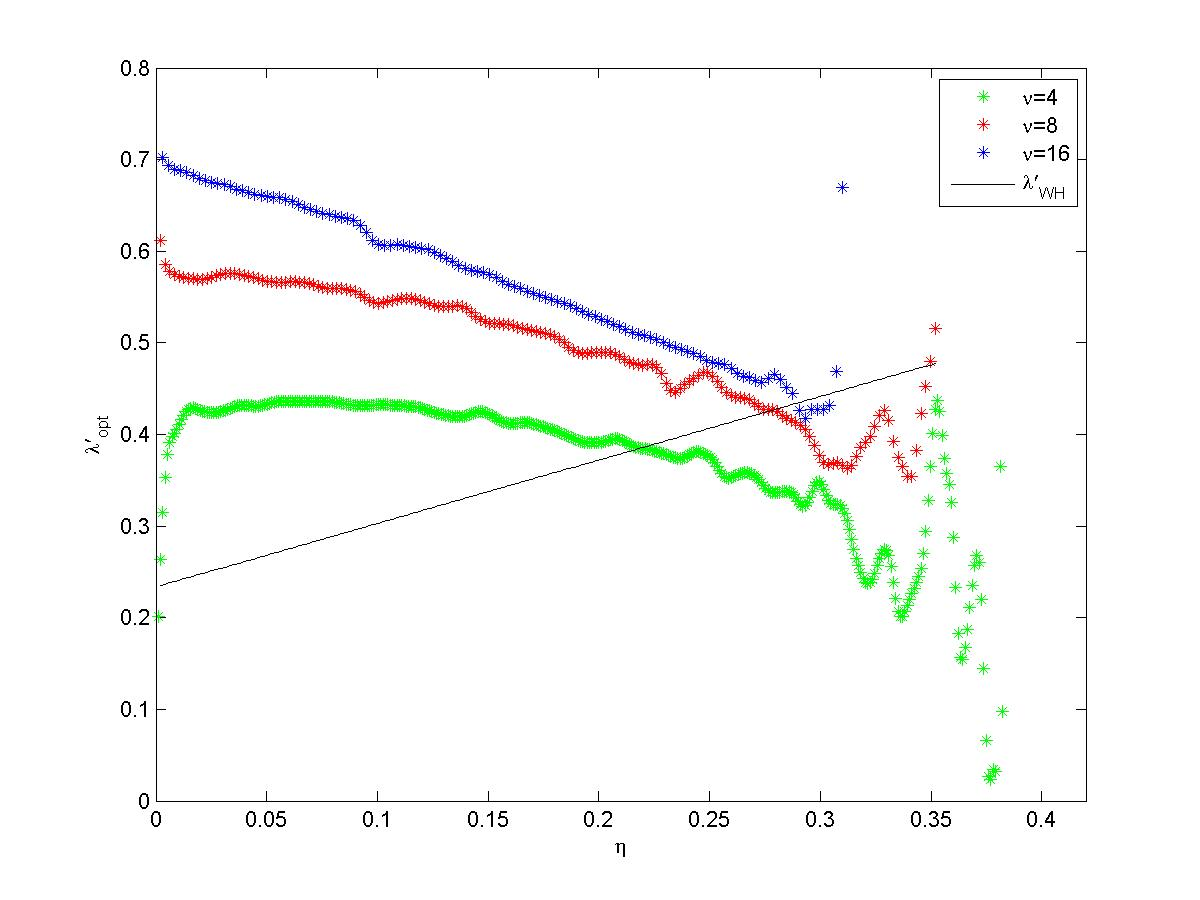
\includegraphics[width=.5\textwidth]{Figures/LambdasInOnePic.jpg}
\caption{The optimal $\lao'$ values for different chain lengths by \eqref{TPT:la:laopt}
and the Wertheim approximation $\lawh'$ by \eqref{TPT:la:laWH}.}
\label{figure:LambdasInOnePic}
\end{figure}


There are four important aspects that have to be considered before one can properly
tackle the problem of approximation:

\id\textbf{$\nu$ dependency.} There are two main classes of approximations:
those which, like the actual $\la$ and $\la'$, only depend on $\e$; and those which also depend
on $\nu$. We call the first class \ep{$\nu$ fix} functions. It will contain $\laf$, $\lae$ and $\las$, which
are approximations to the $\lao'$ for $\nu=4,8$ and $16$, respectively. We also consider
$\lai$, which is a $\nu$ independent approximation, but fitted not only to one
but to all three $\lao'$ at once. 
%The $\infty$ is not meant as an extrapolation.
And then there is the function that contains a
$\nu$ dependency, $\lanu$. We call it simply the \ep{$\nu$ dependent} function. Since
it has the most degrees of freedom, the $\nu$ dependent function must be potentially
superior to the $\nu$ fix functions in an overall context, while the $\nu$ fix functions
will obviously be better for the $\nu$ value they were fitted to (which excludes $\lai$).

\id\textbf{Data selection.} Consider Figure \ref{figure:LambdasInOnePic}. The stars are simulation data
points. We can see that for each $\nu$ the simulation results have increasing noise
towards high $\e$. For $\nu=8$ and especially $\nu=4$ they also change strongly
at low $\e$. We therefore deem it sensible to restrict the fitting efforts to the
areas where $\lao'$ is well-behaved and to neglect data points where $\e$ is too
high and also those with very small $\e$. 
 
\id\textbf{Residual definition.} We want to find the $\la'$ closest to $\lao'$. 
But we need further definition of ``close'' . The key is to minimize some \ep{error function}.
There are of course numerous possibilites
for this error function, of which we chose a simple \ep{least squares fit}, that
is we try to minimize the \ep{root mean square} (RMS) deviation  
%%CHECK: eigentlich muss das noch für \nu-variable \la angegeben werden.
\newcommand\LS{\Dl_{RMS}}
\begin{subequations}
\label{TPT:la:LSQ}
\begin{align}
\LS^\nu\ed{\la'}:=&\sqrt{\frac 1 {K^\nu} \sum_{i=1}^{K^\nu} \rb{\lao'(\enui,\nu)-\la'(\enui,\nu)}^2},
\label{TPT:la:LSQ1}\\
\LS\ed{\la'}:=&\sqrt{\sum_{\nu}\frac 1 {K^\nu}\sum_{i=1}^{K^\nu} \rb{\lao'(\enui,\nu)-\la'(\enui,\nu)}^2}.
\label{TPT:la:LSQ2} 
\end{align} 
\end{subequations}
The two definitions are either for a single $\nu$ or for all $\nu$. We will need
both. It would also be possible to include a weighting function in
\eqref{TPT:la:LSQ} to stress the importance of $\la'$ at some $\e$ values, but since
we do not consider any $\e$ interval to be of higher or lower importance than
another (except for those we already neglected), we have no reason to use such a
function.

\id\textbf{Functional form.} The approximation potential does of course highly depend on
the functional form we allow our approximative functions $\la'$ to take. Wertheim
chose a first order polynomial. One can see in Figure \ref{figure:LambdasInOnePic}
that his coefficients do not reproduce $\lao'$ very accurately (which was never
his intention). But even with better coefficients, the curvature of the
$\lao'$ will not be ideally reproduced. However, a fit of this type is useful.
We call them first order polynomial fit and define
\newcommand\po{{p1}}
\newcommand\lanupo{\la_{\tilde \nu,p1}}
\begin{equation}
\begin{aligned}
\la'_\po:=&c_1^\po+c_2^\po\e.%\\
%\lanupo:=&c_1(\nu)+c_2(\nu)\e.
\end{aligned}
\label{TPT:la:p1}
\end{equation}
For a $\nu$ dependent $\la$, the coefficients will be $\nu$ dependent.
Analogously, we can use a second order polynomial
\newcommand\pt{{p2}}
\newcommand\lanupt{\la_{\tilde \nu,p2}}
\begin{equation}
\begin{aligned}
\la'_\pt:=&c_1^\pt+c_2^\pt\e+c_3^\pt\e^2.%,\\
%\lanupt:=&c_1(\nu)+c_2(\nu)\e+c_3(\nu)\e^2.
\end{aligned}
\label{TPT:la:p2}
\end{equation}
%The different $c_j$ coefficients are not the same in \eqref{TPT:la:p1}
%and \eqref{TPT:la:p2}. 
Finally, we tried a third approach with a Gaussian
bell curve. The motivation to use this function was mostly that the
$\nu=4$ and $\nu=8$ curves for $\lao'$ seemed to increase in decay toward high
$\e$ values while having a maximum at small $\e$. Also, for high $\e$ the polynomial functions
would increase towards infinite values, possibly destroying the decent
results obtained by TPT1, while the exponential curve just returns
the TPT1 compressibility factors for high $\e$. The exponential curve
is given by the parameters
\newcommand\ex{{ex}}
\begin{equation}
\la'_\ex:=c_1^\ex \exp\rb{-\frac{\rb{\e-c_3^\ex}^2}{c_2^\ex}}.
\label{TPT:la:ex}
\end{equation} 

Now we have gathered the proper definitions and data selections to find approximating
functions. 
%Just a quick word on nomenclature: we will call the $\nu$ fix functions
%$\la_{\nu,F}'$ with \mbox{$\nu \in \st{4,8,16,\infty}$} and \mbox{$F \in \st{p1,p2,ex}$}.
%The $\nu$ dependent functions will be called $\la_{\tilde \nu,F}'$.
We will look
at each functional form separately, first establishing the four $\nu$ free approximations
and guessing from them the $\nu$ dependent approximation, which will then be fitted
accordingly. MATLAB$^\circledR$ \cite{Matlab} functions \texttt{fminunc} and
\texttt{fmincon} are used to find the fitting function.

\vskip.3cm
\id\textbf{$\nu$ fix fits.} We collected the data for the first order polynomial,
second order polynomial and Gaussian fit in Tables \ref{TPT:tableP1}, \ref{TPT:tableP2}
and \ref{TPT:tableGauss}, respectively. The RMS values are calculated by \eqref{TPT:la:LSQ1}
for \mbox{$\nu=4,8,16$} and by \eqref{TPT:la:LSQ2} for $\nu=\infty$.

\begin{table}[h]
  \centering
  \caption{Coefficients and RMS deviation for the polynomial fit of first order \eqref{TPT:la:p1}.}
    \begin{tabular}{l | cc | r}
    %\cline{2-3}
         & $c^\po_1$ & $c^\po_2$  & RMS \\[2pt]
    \hline
    & & \\[-.25cm]
    $\nu=4$ & 0.467 & -0.441 & 0.0251\\
    $\nu=8$ & 0.608  & -0.643 & 0.0159\\
    $\nu=16$ & 0.705 &  -0.897 & 0.0052\\[2pt] \hline
    & & \\[-.32cm]
    $\nu=\infty$ & 0.614 &   -0.687 & 0.2932 \\[2pt]
    \hline
    \end{tabular}%
    \label{TPT:tableP1}
\end{table}
% RMS for p1 4: 2.251352e-02
% RMS for p1 8: 1.591368e-02
% RMS for p1 16: 5.212253e-03
% RMS for p1 infty: 2.932301e-01

For the first order polynomial, the case $\nu=16$ can already be well approached. As we can
see in Figure \ref{figure:LambdasInOnePic}, $\lao'$ is close to linear in this case. $\nu=4$,
however, is more problematic. 
%It is possible that this also amounts from the increasing
%oscillations toward higher $\e$.
When we consider the coefficients, we can see that
they show monotonous behavior. They also appear to be close to linear, that is, since
we increased the number $\nu$ exponentially, one could maybe describe them rather well
by a logarithmic function. We will come back to that later.
 
\begin{table}[h]
  \centering
  \caption{Coefficients and RMS deviation for the polynomial fit of second order \eqref{TPT:la:p2}.}
    \begin{tabular}{l | ccc | r}
    %\cline{2-3}
         & $c^\pt_1$ & $c^\pt_2$ & $c^\pt_3$  & RMS \\[2pt]
    \hline
    & & &\\[-.25cm]
    $\nu=4$ & 0.416 & 0.423 & -2.555 & 0.0106\\
    $\nu=8$ & 0.581  & -0.156 & -1.472 & 0.0107\\
    $\nu=16$ & 0.699 &  -0.754 & -0.475 & 0.0041\\[2pt] \hline
    & & & \\[-.32cm]
    $\nu=\infty$ &  0.587 &-0.204 & -1.436 & 0.1830\\[2pt]
    \hline
    \end{tabular}%
    \label{TPT:tableP2}
\end{table}%
% RMS for p2 8: 1.061352e-02
% RMS for p2 4: 1.069520e-02
% RMS for p2 16: 4.146884e-03
% RMS for p2 infty: 1.829798e-01
For the second order polynomial, we can only slightly improve the convergence of the $\nu=16$
fit while especially the $\nu=4$ fit strongly improves. There is also some improvement in the
$\nu=8$ fit. Again, the coefficients follow a monotonous pattern, which is again
close to linear for an exponential increase in $\nu$. 

\begin{table}[h]
  \centering
  \caption{Coefficients and RMS deviation for the Gaussian fit function \eqref{TPT:la:ex}.}
    \begin{tabular}{l | ccc | r}
    %\cline{2-3}
         & $c^\ex_1$ & $c^\ex_2$ & $c^\ex_3$  & RMS \\[2pt]
    \hline
    & & &\\[-.25cm]
    $\nu=4$ & 0.435 & 0.142 & 0.086 & 0.0116 \\
    $\nu=8$ & 0.577 & 0.261 & -0.007 & 0.0105\\
    $\nu=16$ & 0.779 & 0.480 & -0.233 & 0.0042\\[2pt] \hline
    & & & \\[-.32cm]
    $\nu=\infty$ &  0.584 & 0.264 & -0.019 & 0.1832\\[2pt]
    \hline
    \end{tabular}%
    \label{TPT:tableGauss}
\end{table}%
% RMS for exp 4: 1.160153e-02
% RMS for exp 8: 1.050925e-02
% RMS for exp 16: 4.189941e-03
% RMS for exp infty: 1.831906e-01

The relation between the second order polynomial and the Gaussian fit function 
is more interesting. They are both superior to the first order polynomial,
but the Gaussian function describes the case $\nu=8$ slightly better while
it is not as good for the $\nu=4$ case. They are equally good for describing
the case $\nu=16$ and also have similar results for $\nu=\infty$, at least
when only comparing them in RMS value. Considering the Gaussian fit alone,
we find again monotonous behavior in the coefficients. However, this case
seems closer to an actual linear relation between the coefficients and
$\nu$ instead of $\ln\ed{\nu}$. 

The case $\nu=\infty$ is only poorly covered. The worst RMS deviation
for a single $\nu$ is still more than an order of magnitude smaller than the
overall RMS for each approximation. We are interested in a fit that may
interpolate $\lao'$ for $\nu$ values between 4 and 16 (or even extrapolate), so
a $\nu$ dependent fit seems to be the only option. We will lose in accuracy
for the single $\nu$ cases, but we hope to improve the fit for the $\nu=\infty$
case. 

\vskip.3cm
\id\textbf{$\nu$ dependent fits.} After considering the various $\nu$ fix functions, we want to find $\nu$ dependent
versions. We already noted for the two polynomial cases that the coefficients seem to
behave linearly on the logarithmic scale for $\nu$. We therefore assume
\begin{equation}
\begin{aligned}
\la_{\tilde \nu,\po}'%&=\rb{c^\po_{1,1}+c^\po_{1,2}\ln\ed{\nu}}+\rb{c^\po_{2,1}+c^\po_{2,2}\ln\ed{\nu}}\e\\
&=c^\po_1(\nu)+c^\po_2(\nu)\e, \\
c^\po_i(\nu):&=c^\po_{i,1}+c^\po_{i,2}\ln\ed{\nu}
\end{aligned}
\end{equation}
for the first order polynomial. After fitting, we find for the coefficients
\begin{equation}
\begin{aligned}
c^\po_1(\nu)&=0.2446+0.1665\ln\ed{\nu},\\
c^\po_2(\nu)&=0.0187-0.3276\ln\ed{\nu}.
\end{aligned}
\end{equation}
The RMS values can be found in Table \ref{TPT:table:NdepRMS}, as for the other two
fits. We will compare them later.

We have analogously for the second order polynomial
\begin{equation}
\begin{aligned}
\la_{\tilde \nu,\pt}'&=c^\pt_1(\nu)+c^\pt_2(\nu)\e+c^\pt_3(\nu)\e^2, \\
c^\pt_i(\nu):&=c^\pt_{i,1}+c^\pt_{i,2}\ln\ed{\nu}.
\end{aligned}
\end{equation}
The coefficients can be fitted to arrive at
\begin{equation}
\begin{aligned}
c^\pt_1(\nu)&=\ph{-}0.1423+0.2013\ln\ed{\nu},\\
c^\pt_2(\nu)&=\ph{-}1.6104-0.8606\ln\ed{\nu},\\
c^\pt_3(\nu)&=-4.6831+1.5520\ln\ed{\nu}.
\end{aligned}
\end{equation}

In the Gaussian case, the coefficients do not seem to be that well-described with
dependency on $\ln\ed{\nu}$. We will rather use linear relations between the $c^\ex$ and
$\nu$, as already noted above. This means
\begin{equation}
\begin{aligned}
\la_{\tilde \nu,\pt}'&=c_1^\ex(\nu) \exp\rb{-\frac{\rb{\e-c_3^\ex(\nu)}^2}{c_2^\ex(\nu)}},\\
c^\ex_i(\nu):&=c^\ex_{i,1}+c^\ex_{i,2}\nu.
\end{aligned}
\end{equation}
Our coefficient suggestion is then
\begin{equation}
\begin{aligned}
c^\ex_1(\nu)&=0.2319+0.0576\nu,\\
c^\ex_2(\nu)&=0.4216+0.0425\nu,\\
c^\ex_3(\nu)&=0.0732-0.0503\nu.
\end{aligned}
\end{equation}

\begin{table}[h]
  \centering
  \caption{RMS deviations for all $\nu$ dependent fits. RMS values are given for sets of only
  one value for $\nu$ as well as all values of $\nu$ in the row $\nu=\infty$.}
    \begin{tabular}{l | ccc}
    %\cline{2-3}
         & $\la_{\tilde \nu,\po}$ & $\la_{\tilde \nu,\pt}$ & $\la_{\tilde \nu,\ex}$\\[2pt] 
    \hline
    & & \\[-.25cm]
    $\nu=4$ & 0.0244 & 0.0120 & 0.0201 \\
    $\nu=8$ & 0.0258 & 0.0255 & 0.0146 \\
    $\nu=16$ & 0.0057 & 0.0047 & 0.0062\\[2pt] \hline
    & & & \\[-.32cm]
    $\nu=\infty$ &  0.0560 & 0.0422 & 0.0410 \\[2pt]
    \hline
    \end{tabular}%
    \label{TPT:table:NdepRMS}
\end{table}%
% RMS for n dep poly1 (nu=4): 2.447745e-02
% RMS for n dep poly1 (nu=8): 2.579853e-02
% RMS for n dep poly1 (nu=16): 5.703572e-03
% RMS for n dep poly1 (all points): 5.597955e-02
% RMS for n dep poly2 (nu=4): 1.200317e-02
% RMS for n dep poly2 (nu=8): 2.550122e-02
% RMS for n dep poly2 (nu=16): 4.744756e-03
% RMS for n dep poly2 (all points): 4.224914e-02
% RMS for n dep Gauss (nu=4): 2.011305e-02
% RMS for n dep Gauss (nu=8): 1.458760e-02
% RMS for n dep Gauss (nu=16): 6.199412e-03
% RMS for n dep Gauss (all points): 4.090007e-02
Now, we succeeded in finding $\nu$ dependent fits. Comparison of Table \ref{TPT:table:NdepRMS}
to Tables \ref{TPT:tableP1}, \ref{TPT:tableP2} and \ref{TPT:tableGauss} shows that
the loss in accuracy for each isolated $\nu$ is well outweighed by the gain in accuracy
for the overall RMS deviation. The overall deviation is still greater than each single
deviation, but the difference is now roughly a factor of 2 from the worst single $\nu$ approximation
as compared to a factor greater than 10. 

So, finally, there is only the question of which fit is best. The answer, however, is not that
simple. We neither have further experimental nor simulation data to compare the
results to. We try to give a few arguments: First of all, since none of the three
fits is particularly complex, the slightly lesser degree of complexity in the first
order polynomial is not a real advantage. The other two fits are more accurate
in RMS deviation, therefore we recommend one of them. When only considering the overall RMS, the
Gaussian fit offers a faint advantage over the second order polynomial.   

Of course, the maximum degree of accuracy depends on the functional form we offered for the
coefficients. We chose rather vague guesses, due to the fact that we only simulated three
distinct $\nu$. It may have been an advantage that we could identify the coefficients
of the Gaussian fit with isolated properties of the resulting curve: location of maximum, value of
maximum and variancy (actually, $2$ times the variancy). The same applies to
the first order polynomial, while for the second order polynomial we can only
properly guess the local behavior at $\e=0$ from the function.


\section{Conclusion and Outlook}
\label{Con}
We introduced the framework of graph theory and the Mayer formalism. From there, we
followed Wertheim's reasoning to find more convenient expressions for the grand
canonical EOS and the free energy in a system governed by highly directional
attractive forces. By means of thermodynamic perturbation theory, we derived equations
of state of first and second TPT order, where we fitted a parameter in the latter
to simulation data. The results are three good approximations within the range of
our data. We did not check how well the approximation is for different $\nu$ values
or how strongly the optimum depends on $\be$ and $V$. This may be a topic for further
research.

Within our approximation, it would be interesting to closer observe the $\nu$ dependency
of the fitting function coefficients. With more data points, more elaborate guesses
could be possible, maybe also for the fitting functions themselves. It could also
be interesting to find expressions for $\la'$ that are closer to Wertheim's
analytical value for $\la$ and its derivative in the case \mbox{$\e \rightarrow 0$}. By that, a compromise
between pure mathematical approximation and physical reasoning may be possible.

\section*{Acknowledgment}
I want to thank Professor J. Groß for his support and Mr. Wasilios Zmpitas for
his introduction to the topic and everything following that.   


%\clearpage
% \bibliographystyle{apalikenotitle}
\bibliographystyle{ieeetr}
% \begin{thebibliography}
\bibliography{BibForsch2}

\end{document}

